%%
%% Reminder: for minor typo changes, you should use 
%% {old}{new}
%%   or
%% {new}
%%   or
%% {old}
%%
%% Using delete followed by update instead of replace is wrong.
%%
%%%%%%%%%%%%%%%%%%%%%%%%%%%%%%%%%%%%%%%%%%%%%%%%%%%%%%%%%%%


\chapter{One-Sided Communications}
\mpitermtitleindexsubmain{one-sided}{communication}
\label{chap:one-side-2}
\label{sec:one-side-2}

\section{Introduction}

\mpitermdefni{Remote Memory Access}\mpitermdefindex{Remote Memory Access!see RMA@see \RMA/}
\mpitermdefni{(\RMA/)}\mpitermdefindex{RMA@\RMA/}\mpitermdefindex{communication!RMA@\RMA/}
extends the communication mechanisms of \MPI/ by
allowing one \mpi/ process to specify all communication parameters, both for
the sending side and for the receiving side.
This mode of communication facilitates the coding of some applications
with dynamically changing data access patterns
where the data distribution is fixed or slowly changing.  
In such a case,
each \mpi/ process can compute what data it needs to access or 
to update at
other \mpi/ processes.  
However, the
programmer may not be able to easily determine which data in an \mpi/ process
may need to be accessed or to be updated by operations initiated by a
different \mpi/ process, and may not even know which \mpi/ processes may perform
such updates.
Thus, the transfer parameters are all available only on one side.
Regular send/receive communication requires matching operations by
sender and receiver.
In order to issue the matching operations, an application needs to
distribute the transfer parameters. 
This distribution may
require all \mpi/ processes to participate in a time-consuming global
computation,
or to poll for potential communication requests to
receive and upon which to act periodically.
The use of \RMA/ communication operations avoids the need for
global computations or explicit polling.
A generic example of this nature is the execution of an assignment of
the form
\code{A = B(map)}, where \code{map} is a permutation vector, and \code{A},
\code{B}, and \code{map} are distributed
in the same manner.  

Message-passing communication achieves two effects:
\mpiterm{communication} of data from sender to
receiver and 
\mpiterm{synchronization} of sender 
with receiver.
The \RMA/ design separates these two functions.
The following communication calls are provided:
\begin{itemize}
\item Remote write: \mpifunc{MPI\_PUT}, \mpifunc{MPI\_RPUT}
\item Remote read: \mpifunc{MPI\_GET}, \mpifunc{MPI\_RGET}
\item Remote update: \mpifunc{MPI\_ACCUMULATE}, \mpifunc{MPI\_RACCUMULATE}
\item Remote read and update: \mpifunc{MPI\_GET\_ACCUMULATE}, \mpifunc{MPI\_RGET\_ACCUMULATE},
and \mpifunc{MPI\_FETCH\_AND\_OP}
\item Remote atomic swap: \mpifunc{MPI\_COMPARE\_AND\_SWAP}
\end{itemize}
This chapter refers to an operations set that includes all remote update,
remote read and update, and remote atomic swap operations as
``accumulate'' operations.

\MPI/ supports two fundamentally different \mpitermni{memory models}\mpitermindex{memory model}:
\mpitermni{separate}\mpitermindex{separate memory model}\mpitermindex{memory model!separate}
and \mpitermni{unified}\mpitermindex{unified memory model}\mpitermindex{memory model!unified}.
The separate model makes no assumption about memory consistency and is
highly portable. This model is similar to that of weakly coherent memory
systems: the user must impose correct ordering of memory accesses
through synchronization calls. The
unified model can exploit cache-coherent hardware and
hardware-accelerated, one-sided operations that are commonly available
in high-performance systems.
The two different models are discussed in detail in
Section~\ref{sec:1sided-memmodel}.
Both models support several synchronization calls to support
different synchronization styles.

The design of the \RMA/ functions allows implementors to take 
advantage of fast or asynchronous communication mechanisms provided by various
platforms, such as coherent or noncoherent shared memory, DMA
engines, hardware-supported put/get operations, and communication
coprocessors.  The most frequently used \RMA/
communication mechanisms can be layered on top of message-passing.  
However, certain 
\RMA/ functions might need support for asynchronous communication agents in
software (handlers, threads, etc.) in a distributed memory environment.

We shall denote by \mpitermdef{origin} or \mpitermni{origin process} the \MPI/ process that calls an \RMA/ procedure,
and by \mpitermdef{target} or \mpitermni{target process} the \MPI/ process whose memory is accessed.
Thus, in a put
operation, \mpicode{source~=~origin} and \mpicode{destination~=~target}; in a
get operation, \mpicode{source~=~target} and \mpicode{destination~=~origin}.

\section{Initialization}
\label{sec:one-side-2:intro}


\MPI/ provides
the following window initialization
functions: \mpifunc{MPI\_WIN\_CREATE},
\mpifunc{MPI\_WIN\_ALLOCATE},
\mpifunc{MPI\_WIN\_ALLOCATE\_SHARED},
and\flushline % fix for margin 
\mpifunc{MPI\_WIN\_CREATE\_DYNAMIC}, which are collective over the group of an
intra\hyphen/communicator.
\mpifunc{MPI\_WIN\_CREATE}
allows each \mpi/ process to specify a ``window'' in its
memory that is made available for accesses by other \mpi/
processes.
The call returns an opaque object
that represents the group of \mpi/
processes that own and access the set of windows,
and the attributes of each window, as specified by the initialization call.
\mpifunc{MPI\_WIN\_ALLOCATE} and \mpifunc{MPI\_WIN\_ALLOCATE\_SHARED} differ from
\mpifunc{MPI\_WIN\_CREATE} in that the user does not pass allocated
memory; instead \mpifunc{MPI\_WIN\_ALLOCATE} and \mpifunc{MPI\_WIN\_ALLOCATE\_SHARED} return a
pointer to memory allocated by the \MPI/ implementation.
\mpifunc{MPI\_WIN\_ALLOCATE\_SHARED} differs from
\mpifunc{MPI\_WIN\_ALLOCATE} in that the allocated memory is guaranteed to be
accessible from all \mpi/ processes in the window's group with direct load/store accesses. Some
restrictions may apply to the specified communicator.
\mpifunc{MPI\_WIN\_CREATE\_DYNAMIC} creates a window that allows the
user to dynamically control which memory is exposed by the window.

\subsection{Window Creation}
\mpitermtitleindex{window!creation}
\label{chap:one-side-2:win_create}

\cdeclmainindex{MPI\_Win}\cdeclmainindex{TYPE(MPI\_Win)}%
\cdeclindex{MPI\_Aint}%
\begin{funcdef}{MPI\_WIN\_CREATE}{(\mbox{base}, \mbox{size}, \mbox{disp\_unit}, \mbox{info}, \mbox{comm}, \mbox{win})}
\funcarg{\IN}{base}{initial address of window (choice)}
\funcarg{\IN}{size}{size of window in bytes (nonnegative integer)}
\funcarg{\IN}{disp\_unit}{local unit size for displacements, in bytes (positive integer)}
\funcarg{\IN}{info}{info argument (handle)}
\funcarg{\IN}{comm}{intra-communicator (handle)}
\funcarg{\OUT}{win}{window object (handle)}
\end{funcdef}
\mpibindmain{MPI\_Win\_create}{(\gb{}void~*base, MPI\_Aint~size, int~disp\_unit, MPI\_Info~info, MPI\_Comm~comm, MPI\_Win~*win)}
\MPIbindindex{MPI\_Win\_create\_c}
\mpibindmain{MPI\_Win\_create\_c}{(\gb{}void~*base, MPI\_Aint~size, MPI\_Aint~disp\_unit, MPI\_Info~info, MPI\_Comm~comm, MPI\_Win~*win)}
\mpifnewbindmain{MPI\_Win\_create}{(base, size, disp\_unit, info, comm, win, ierror) \fargs TYPE(*), DIMENSION(..), ASYNCHRONOUS\ ::\ \mbox{base}\fnarg{}INTEGER(KIND=MPI\_ADDRESS\_KIND), INTENT(IN)\ ::\ \mbox{size}\fnarg{}INTEGER, INTENT(IN)\ ::\ \mbox{disp\_unit}\fnarg{}TYPE(MPI\_Info), INTENT(IN)\ ::\ \mbox{info}\fnarg{}TYPE(MPI\_Comm), INTENT(IN)\ ::\ \mbox{comm}\fnarg{}TYPE(MPI\_Win), INTENT(OUT)\ ::\ \mbox{win}\fnfinalarg{}INTEGER, OPTIONAL, INTENT(OUT)\ ::\ \mbox{ierror}}
\mpifnewbindmain{MPI\_Win\_create}{(base, size, disp\_unit, info, comm, win, ierror) !(\_c) \fargs TYPE(*), DIMENSION(..), ASYNCHRONOUS\ ::\ \mbox{base}\fnarg{}INTEGER(KIND=MPI\_ADDRESS\_KIND), INTENT(IN)\ ::\ \mbox{size}, \mbox{disp\_unit}\fnarg{}TYPE(MPI\_Info), INTENT(IN)\ ::\ \mbox{info}\fnarg{}TYPE(MPI\_Comm), INTENT(IN)\ ::\ \mbox{comm}\fnarg{}TYPE(MPI\_Win), INTENT(OUT)\ ::\ \mbox{win}\fnfinalarg{}INTEGER, OPTIONAL, INTENT(OUT)\ ::\ \mbox{ierror}}
\mpifbindmain{MPI\_WIN\_CREATE}{(BASE, SIZE, DISP\_UNIT, INFO, COMM, WIN, IERROR) \fargs <type> \mbox{BASE(*)}\fnarg{}INTEGER(KIND=MPI\_ADDRESS\_KIND) \mbox{SIZE}\fnfinalarg{}INTEGER \mbox{DISP\_UNIT}, \mbox{INFO}, \mbox{COMM}, \mbox{WIN}, \mbox{IERROR}}

This procedure is collective over the group of
\mpiarg{comm}.  It returns a handle to a window that can be used by the
\mpi/ processes in this group to perform \RMA/ operations.  Each \mpi/ process specifies
a window of existing memory that it exposes to \RMA/ accesses by any \mpi/
processes in the group of
\mpiarg{comm}.
The window consists of \mpiarg{size} bytes,
starting at address \mpiarg{base}.
In C, \mpiarg{base} is the starting
address of a memory region. 
In Fortran, one can pass the first element of a memory region
or a whole array, which must be `simply contiguous' 
(for `simply contiguous,' see also 
\sectionref{sec:misc-sequence}).
An \mpi/ process may elect to expose no memory by
specifying \mpiarg{size}\mpicode{ = 0}.

The displacement unit argument
is provided to facilitate address arithmetic in \RMA/
operations: the target displacement argument of an \RMA/ operation is
scaled by the factor \mpiarg{disp\_unit} specified by the target
process, at window creation.

\begin{rationale}
The window size is specified using an address-sized integer,
rather than a basic integer type, to allow windows that span more memory than
can be described with a basic integer type.
\end{rationale}

\begin{users}
Common choices for \mpiarg{disp\_unit}
are 1 (no scaling), and (in C syntax) \code{sizeof(type)}, for a
window that consists of an array of elements of type \code{type}.  The
latter
choice will allow one to use array indices in \RMA/ calls,
and have those scaled correctly to byte displacements, even in a
heterogeneous environment.
\end{users}

The \mpiarg{info} argument provides
optimization hints to the runtime about the expected
usage pattern of the window.
The following info keys are predefined:

\begin{description}
\item[\infokeymain{no\_locks} (boolean, default: \infoval{false}):]if set to \infoval{true},
then the implementation may assume that passive target synchronization (i.e.,
\mpifunc{MPI\_WIN\_LOCK}, \mpifunc{MPI\_WIN\_LOCK\_ALL}) will not be used on
the given window. This implies that this window is not used for 3-party
communication, and \RMA/ can be implemented with no (less) asynchronous
agent activity at this \MPI/ process.
\item[\infokeymain{accumulate\_ordering} (string, default \infovalskip{rar,raw,war,waw}):]controls the ordering of accumulate 
operations at the target.  See Section~\ref{sec:1sided-ordering} for details.
\item[\infokeymain{accumulate\_ops} (string, default: \infoval{same\_op\_no\_op}):]if set to \infovalmain{same\_op},
the implementation will assume that all concurrent accumulate calls
to the same target address will use the same operator. If set to
\infovalmain{same\_op\_no\_op}, then the implementation will assume that
all concurrent accumulate calls to the same target address will use the
same operator or \mpiconst{MPI\_NO\_OP}. This can eliminate the need to
protect access for certain operators where the hardware can
guarantee atomicity.
{\sloppy %ALLOWLATEX%
\item[\infokeymain{mpi\_accumulate\_granularity} (integer, default \code{0}):]provides a hint to implementations about the desired synchronization granularity for accumulate operations, i.e., the size of memory ranges in bytes for which the implementation should acquire a synchronization primitive to ensure atomicity of updates.
If the specified granularity is not divisible by the size of the type used in an accumulate operation, it should be treated as if it was the next multiple of the element size.
For example, a granularity of \infovalskip{1} byte  should be treated as \infovalskip{8} in an accumulate operation using \type{MPI\_UINT64\_T}.
By default, this info key is set to \infovalskip{0}, which leaves the choice of synchronization granularity to the implementation.
If specified, all \mpi/ processes in the group of a window must supply the same value.

}
%
\begin{users}
Small synchronization granularities may provide improved latencies for accumulate operations with few elements and potentially increase concurrency of updates, at the cost of lower throughput.
For example, a value matching the size of a type involved in an accumulate operation may enable implementations to use atomic memory operations instead of mutual exclusion devices.
Larger synchronization granularities may yield higher throughput of accumulate operation with large numbers of elements due to lower synchronization costs, potentially at the expense of higher latency for accumulate operations with few elements, e.g., if atomic memory operations are not employed.
By dividing larger accumulate operations into smaller segments, concurrent accumulate operations to the same window memory may update different segments in parallel.
\end{users}
%
\begin{implementors}
Implementations are encouraged to avoid mutual exclusion devices in cases where the granularity is small enough to warrant the use of atomic memory operations.
For larger granularities, implementations should use this info value as a hint to partition the window memory into zones of mutual exclusion to enable segmentation of large accumulate operations.
\end{implementors}
%
\item[\infokeymain{same\_size} (boolean, default: \infoval{false}):]if set to \infoval{true},
then the implementation may assume that the argument \mpiarg{size} is
identical on all \mpi/ processes, and that all \mpi/ processes have provided this
info key with the same value.
\item[\infokeymain{same\_disp\_unit} (boolean, default: \infoval{false}):]if set to \infoval{true},
then the implementation
may assume that the argument \mpiarg{disp\_unit}
is identical on all \mpi/ processes, and
that all \mpi/ processes have provided this info key with the same value.
\item[\infokey{mpi\_assert\_memory\_alloc\_kinds} (string, not set by default):]
If set, the implementation may assume that the memory for all
communication buffers passed to \MPI/ operations performed by the calling \MPI/
process on the given window will use only the memory allocation kinds
listed in the value string.
See Section~\ref{subsec:mem_alloc_kinds}.
This info hint also applies to the window buffer provided in a call to
\mpifunc{MPI\_WIN\_CREATE} or \mpifunc{MPI\_WIN\_ATTACH}. It does not
apply to the memory
allocated in a call to \mpifunc{MPI\_WIN\_ALLOCATE} or
\mpifunc{MPI\_WIN\_ALLOCATE\_SHARED}.
\end{description}

\begin{users}
The info query mechanism described in Section~\ref{subsec:window-info}
can be used to query the specified info arguments
for
windows that have been
passed to a library. It is recommended that libraries check attached
info keys for each passed window.
\end{users}

The various \mpi/ processes in the group of
\mpiarg{comm} may specify completely different
target windows, in location, size, displacement
units, and info arguments. 
As long as all the get, put and accumulate accesses 
to a particular \mpi/ process fit their
specific target window this should pose no problem.
The same area in memory may appear in multiple windows, each
associated with a different window object.  However, concurrent
communications to distinct, overlapping windows may lead to
undefined
results.

Implementations may make the memory provided by the user available for load/store accesses
by \MPI/ processes in the same \mpitermni{shared memory domain}\mpitermindex{shared memory!domain}.
A communicator of such \MPI/ processes can be constructed as described in Section~\ref{subsec:context-intracomconst} using \mpifunc{MPI\_COMM\_SPLIT\_TYPE}.
Pointers to access a \mpitermni{shared memory segment}\mpitermindex{shared memory!segment} can be queried
using \mpifunc{MPI\_WIN\_SHARED\_QUERY}.

\begin{rationale}
The reason for specifying the memory that may be accessed from another
\mpi/ process in an \RMA/ operation is to permit the programmer to specify
what memory can be a target of \RMA/ operations and for the
implementation to enforce that specification.  For example, with this
definition, a server \mpi/ process can safely allow a client \mpi/ process to use
\RMA/ operations, knowing that (under the assumption that the \MPI/
implementation does enforce the specified limits on the exposed
memory) an error in the client cannot affect any memory other than
what was explicitly exposed.  
\end{rationale}

\begin{users}
A window can be created in any part of the \mpi/ process memory.  However,
on some systems, the performance of windows in
memory allocated by \mpifunc{MPI\_ALLOC\_MEM} 
(\sectionref{sec:misc-memalloc}) will be better.
Also, on some systems, performance is improved when window boundaries
are aligned at ``natural'' boundaries (word, double-word, cache line,
page frame, etc.).
\end{users}

\begin{implementors}
In cases where \RMA/ operations use different mechanisms in different
memory areas (e.g., load/store accesses in a \mpitermni{shared memory segment}\mpitermindex{shared memory!segment}, and an
asynchronous handler in private memory), the \mpifunc{MPI\_WIN\_CREATE}
call needs to figure out which type of memory is used for the
window.  To do so, \MPI/ maintains, internally, the
list of memory segments allocated by \mpifunc{MPI\_ALLOC\_MEM}, or by
other, implementation-specific,
mechanisms, together with information 
on the type of memory segment allocated.  When a call to 
\mpifunc{MPI\_WIN\_CREATE} occurs, then \MPI/ checks which segment
contains each window, and decides, accordingly, which mechanism to use
for \RMA/ operations.

Vendors may provide additional, implementation-specific mechanisms to
allocate or to specify memory regions that are preferable for use in
one-sided communication. In particular, such mechanisms can be used to
place static variables into such preferred regions.

Implementors should document any performance impact of window alignment.
\end{implementors}

\subsection{Window That Allocates Memory}
\mpitermtitleindex{window!allocation}
\mpitermindex{memory!allocation}
\label{sec:winalloc}

%% Alloc_mem uses baseptr, which distinguishes this from the base in win_create
%% The argument signature of this routine follows that for MPI_Alloc_mem; don't 
%% make any changes that make this routine inconsistent with MPI_Alloc_mem.

\cdeclmainindex{MPI\_Win}\cdeclmainindex{TYPE(MPI\_Win)}%
\cdeclindex{MPI\_Aint}%
\begin{funcdef}{MPI\_WIN\_ALLOCATE}{(\mbox{size}, \mbox{disp\_unit}, \mbox{info}, \mbox{comm}, \mbox{baseptr}, \mbox{win})}
\funcarg{\IN}{size}{size of window in bytes (nonnegative integer)}
\funcarg{\IN}{disp\_unit}{local unit size for displacements, in bytes (positive integer)}
\funcarg{\IN}{info}{info argument (handle)}
\funcarg{\IN}{comm}{intra-communicator (handle)}
\funcarg{\OUT}{baseptr}{initial address of window (choice)}
\funcarg{\OUT}{win}{window object (handle)}
\end{funcdef}
\mpibindmain{MPI\_Win\_allocate}{(\gb{}MPI\_Aint~size, int~disp\_unit, MPI\_Info~info, MPI\_Comm~comm, void~*baseptr, MPI\_Win~*win)}
\MPIbindindex{MPI\_Win\_allocate\_c}
\mpibindmain{MPI\_Win\_allocate\_c}{(\gb{}MPI\_Aint~size, MPI\_Aint~disp\_unit, MPI\_Info~info, MPI\_Comm~comm, void~*baseptr, MPI\_Win~*win)}
\mpifnewbindmain{MPI\_Win\_allocate}{(size, disp\_unit, info, comm, baseptr, win, ierror) \fargs USE, INTRINSIC\ ::\ ISO\_C\_BINDING, ONLY : C\_PTR \\ INTEGER(KIND=MPI\_ADDRESS\_KIND), INTENT(IN)\ ::\ \mbox{size}\fnarg{}INTEGER, INTENT(IN)\ ::\ \mbox{disp\_unit}\fnarg{}TYPE(MPI\_Info), INTENT(IN)\ ::\ \mbox{info}\fnarg{}TYPE(MPI\_Comm), INTENT(IN)\ ::\ \mbox{comm}\fnarg{}TYPE(C\_PTR), INTENT(OUT)\ ::\ \mbox{baseptr}\fnarg{}TYPE(MPI\_Win), INTENT(OUT)\ ::\ \mbox{win}\fnfinalarg{}INTEGER, OPTIONAL, INTENT(OUT)\ ::\ \mbox{ierror}}
\mpifnewbindmain{MPI\_Win\_allocate}{(size, disp\_unit, info, comm, baseptr, win, ierror) !(\_c) \fargs USE, INTRINSIC\ ::\ ISO\_C\_BINDING, ONLY : C\_PTR \\ INTEGER(KIND=MPI\_ADDRESS\_KIND), INTENT(IN)\ ::\ \mbox{size}, \mbox{disp\_unit}\fnarg{}TYPE(MPI\_Info), INTENT(IN)\ ::\ \mbox{info}\fnarg{}TYPE(MPI\_Comm), INTENT(IN)\ ::\ \mbox{comm}\fnarg{}TYPE(C\_PTR), INTENT(OUT)\ ::\ \mbox{baseptr}\fnarg{}TYPE(MPI\_Win), INTENT(OUT)\ ::\ \mbox{win}\fnfinalarg{}INTEGER, OPTIONAL, INTENT(OUT)\ ::\ \mbox{ierror}}
\mpifbindmain{MPI\_WIN\_ALLOCATE}{(SIZE, DISP\_UNIT, INFO, COMM, BASEPTR, WIN, IERROR) \fargs INTEGER(KIND=MPI\_ADDRESS\_KIND) \mbox{SIZE}, \mbox{BASEPTR}\fnfinalarg{}INTEGER \mbox{DISP\_UNIT}, \mbox{INFO}, \mbox{COMM}, \mbox{WIN}, \mbox{IERROR}\mpifoverloadOnlyInAnnex{\>INTERFACE MPI\_WIN\_ALLOCATE \\ \>\>SUBROUTINE MPI\_WIN\_ALLOCATE(SIZE, DISP\_UNIT, INFO, COMM, BASEPTR, \& \\ \>\>\>\>WIN, IERROR) \\ \>\>\>IMPORT :: MPI\_ADDRESS\_KIND \\ \>\>\>INTEGER :: DISP\_UNIT, INFO, COMM, WIN, IERROR \\ \>\>\>INTEGER(KIND=MPI\_ADDRESS\_KIND) :: SIZE, BASEPTR \\ \>\>END SUBROUTINE \\ \>\>SUBROUTINE MPI\_WIN\_ALLOCATE\_CPTR(SIZE, DISP\_UNIT, INFO, COMM, BASEPTR, \& \\ \>\>\>\>WIN, IERROR) \\ \>\>\>USE, INTRINSIC :: ISO\_C\_BINDING, ONLY : C\_PTR \\ \>\>\>IMPORT :: MPI\_ADDRESS\_KIND \\ \>\>\>INTEGER :: DISP\_UNIT, INFO, COMM, WIN, IERROR \\ \>\>\>INTEGER(KIND=MPI\_ADDRESS\_KIND) :: SIZE \\ \>\>\>TYPE(C\_PTR) :: BASEPTR \\ \>\>END SUBROUTINE \\ \>END INTERFACE}}

%% WDG - This follows the Fortran binding for MPI_Alloc_mem, which
%% views base (baseptr in alloc_mem) as an address-sized integer in
%% Fortran.  If there is a change in Alloc_mem to use new Fortran
%% interfaces, this binding should follow the same approach

This procedure is collective over the group of
\mpiarg{comm}. On each \mpi/ process, it allocates memory of at least
\mpiarg{size} bytes and returns a pointer to it along with a handle to a new window that
can be used by all \mpi/ processes in the group of \mpiarg{comm} to perform \RMA/
operations.  The returned memory consists of \mpiarg{size} bytes local
to each \mpi/ process, starting at address \mpiarg{baseptr} and is associated
with the window as if the user called \mpifunc{MPI\_WIN\_CREATE} on
existing memory. The size argument may be different at each \mpi/ process and
\mpiarg{size}\mpicode{ = 0} is valid; however, a library might allocate and expose
more memory in order to create a fast, globally symmetric allocation.
The discussion of and rationales for \mpifunc{MPI\_ALLOC\_MEM} and
\mpifunc{MPI\_FREE\_MEM} in Section~\ref{sec:misc-memalloc} also apply to
\mpifunc{MPI\_WIN\_ALLOCATE}; in particular, see the rationale in
Section~\ref{sec:misc-memalloc} for an explanation of the type used for
\mpiarg{baseptr}.

Implementations may make allocated memory available for load/store accesses
by \MPI/ processes in the same \mpitermni{shared memory domain}\mpitermindex{shared memory!domain}.
A communicator of such \MPI/ processes can be constructed as described in Section~\ref{subsec:context-intracomconst} using \mpifunc{MPI\_COMM\_SPLIT\_TYPE}.
Pointers to access a \mpitermni{shared memory segment}\mpitermindex{shared memory!segment} can be queried
using \mpifunc{MPI\_WIN\_SHARED\_QUERY}.
If \mpiterm{shared memory} is available
it is not guaranteed to be \mpitermni{contiguous}\mpitermindex{shared memory!contiguous} (see Section~\ref{sec:winallocshared}).

The \mpiarg{info} argument can be used to specify hints
similar to the \mpiarg{info} argument for \mpifunc{MPI\_WIN\_CREATE} and
\mpifunc{MPI\_ALLOC\_MEM}.

\mpitermindex{memory!alignment}\mpitermindex{alignment}
The default memory alignment requirements and the
\infokey{mpi\_minimum\_memory\_alignment} \mpiarg{info} key described
for \mpifunc{MPI\_ALLOC\_MEM} in Section~\ref{sec:misc-memalloc} apply to
all \mpi/ processes with nonzero \mpiarg{size} argument.
 
If the Fortran compiler provides \ftype{TYPE(C\_PTR)}, 
then the following generic interface must be provided in the \code{mpi}
module and should be provided in the (deprecated) \code{mpif.h} include file through overloading, 
i.e., with the same routine name as the
routine with \mpiftypekind{ADDRESS} \code{BASEPTR},
but with a different specific procedure name:
 
\begin{verbatim}
INTERFACE MPI_WIN_ALLOCATE
    SUBROUTINE MPI_WIN_ALLOCATE(SIZE, DISP_UNIT, INFO, COMM, BASEPTR, &
            WIN, IERROR)
        IMPORT :: MPI_ADDRESS_KIND
        INTEGER :: DISP_UNIT, INFO, COMM, WIN, IERROR
        INTEGER(KIND=MPI_ADDRESS_KIND) :: SIZE, BASEPTR
    END SUBROUTINE
    SUBROUTINE MPI_WIN_ALLOCATE_CPTR(SIZE, DISP_UNIT, INFO, COMM, BASEPTR, &
            WIN, IERROR)
        USE, INTRINSIC :: ISO_C_BINDING, ONLY : C_PTR
        IMPORT :: MPI_ADDRESS_KIND
        INTEGER :: DISP_UNIT, INFO, COMM, WIN, IERROR
        INTEGER(KIND=MPI_ADDRESS_KIND) :: SIZE
        TYPE(C_PTR) :: BASEPTR
    END SUBROUTINE
END INTERFACE
\end{verbatim}

 
The base procedure name of this overloaded function is
\mpifuncmain{MPI\_WIN\_ALLOCATE\_CPTR}. The implied specific procedure
names
are described in \sectionref{sec:f90:linker-names}.

\begin{rationale}
By allocating (potentially aligned) memory instead of allowing the user
to pass in an arbitrary buffer, this call can improve the performance
for systems with remote direct memory access. 
This also permits the collective allocation of memory and
  supports what is sometimes called the ``symmetric allocation'' model
  that can be more scalable (for example, the implementation can
  arrange to return an address for the allocated memory that is the
  same on all \mpi/ processes).
\end{rationale}

\subsection{Window That Allocates Shared Memory}
\mpitermtitleindexmainsub{window}{shared memory!window}
\mpitermindex{memory!allocation}
\mpitermtitleindexmainsub{window}{shared memory allocation}
\label{sec:winallocshared}

%% Alloc_mem uses baseptr, which distinguishes this from the base in win_create
\cdeclmainindex{MPI\_Win}\cdeclmainindex{TYPE(MPI\_Win)}%
\cdeclindex{MPI\_Aint}%
\begin{funcdef}{MPI\_WIN\_ALLOCATE\_SHARED}{(\mbox{size}, \mbox{disp\_unit}, \mbox{info}, \mbox{comm}, \mbox{baseptr}, \mbox{win})}
\funcarg{\IN}{size}{size of local window in bytes (nonnegative integer)}
\funcarg{\IN}{disp\_unit}{local unit size for displacements, in bytes (positive integer)}
\funcarg{\IN}{info}{info argument (handle)}
\funcarg{\IN}{comm}{intra-communicator (handle)}
\funcarg{\OUT}{baseptr}{address of local allocated window segment (choice)}
\funcarg{\OUT}{win}{window object (handle)}
\end{funcdef}
\mpibindmain{MPI\_Win\_allocate\_shared}{(\gb{}MPI\_Aint~size, int~disp\_unit, MPI\_Info~info, MPI\_Comm~comm, void~*baseptr, MPI\_Win~*win)}
\MPIbindindex{MPI\_Win\_allocate\_shared\_c}
\mpibindmain{MPI\_Win\_allocate\_shared\_c}{(\gb{}MPI\_Aint~size, MPI\_Aint~disp\_unit, MPI\_Info~info, MPI\_Comm~comm, void~*baseptr, MPI\_Win~*win)}
\mpifnewbindmain{MPI\_Win\_allocate\_shared}{(size, disp\_unit, info, comm, baseptr, win, ierror) \fargs USE, INTRINSIC\ ::\ ISO\_C\_BINDING, ONLY : C\_PTR \\ INTEGER(KIND=MPI\_ADDRESS\_KIND), INTENT(IN)\ ::\ \mbox{size}\fnarg{}INTEGER, INTENT(IN)\ ::\ \mbox{disp\_unit}\fnarg{}TYPE(MPI\_Info), INTENT(IN)\ ::\ \mbox{info}\fnarg{}TYPE(MPI\_Comm), INTENT(IN)\ ::\ \mbox{comm}\fnarg{}TYPE(C\_PTR), INTENT(OUT)\ ::\ \mbox{baseptr}\fnarg{}TYPE(MPI\_Win), INTENT(OUT)\ ::\ \mbox{win}\fnfinalarg{}INTEGER, OPTIONAL, INTENT(OUT)\ ::\ \mbox{ierror}}
\mpifnewbindmain{MPI\_Win\_allocate\_shared}{(size, disp\_unit, info, comm, baseptr, win, ierror) !(\_c) \fargs USE, INTRINSIC\ ::\ ISO\_C\_BINDING, ONLY : C\_PTR \\ INTEGER(KIND=MPI\_ADDRESS\_KIND), INTENT(IN)\ ::\ \mbox{size}, \mbox{disp\_unit}\fnarg{}TYPE(MPI\_Info), INTENT(IN)\ ::\ \mbox{info}\fnarg{}TYPE(MPI\_Comm), INTENT(IN)\ ::\ \mbox{comm}\fnarg{}TYPE(C\_PTR), INTENT(OUT)\ ::\ \mbox{baseptr}\fnarg{}TYPE(MPI\_Win), INTENT(OUT)\ ::\ \mbox{win}\fnfinalarg{}INTEGER, OPTIONAL, INTENT(OUT)\ ::\ \mbox{ierror}}
\mpifbindmain{MPI\_WIN\_ALLOCATE\_SHARED}{(SIZE, DISP\_UNIT, INFO, COMM, BASEPTR, WIN, IERROR) \fargs INTEGER(KIND=MPI\_ADDRESS\_KIND) \mbox{SIZE}, \mbox{BASEPTR}\fnfinalarg{}INTEGER \mbox{DISP\_UNIT}, \mbox{INFO}, \mbox{COMM}, \mbox{WIN}, \mbox{IERROR}\mpifoverloadOnlyInAnnex{\>INTERFACE MPI\_WIN\_ALLOCATE\_SHARED \\ \>\>SUBROUTINE MPI\_WIN\_ALLOCATE\_SHARED(SIZE, DISP\_UNIT, INFO, COMM, \& \\ \>\>\>\>BASEPTR, WIN, IERROR) \\ \>\>\>IMPORT :: MPI\_ADDRESS\_KIND \\ \>\>\>INTEGER :: DISP\_UNIT, INFO, COMM, WIN, IERROR \\ \>\>\>INTEGER(KIND=MPI\_ADDRESS\_KIND) :: SIZE, BASEPTR \\ \>\>END SUBROUTINE \\ \>\>SUBROUTINE MPI\_WIN\_ALLOCATE\_SHARED\_CPTR(SIZE, DISP\_UNIT, INFO, COMM, \& \\ \>\>\>\>BASEPTR, WIN, IERROR) \\ \>\>\>USE, INTRINSIC :: ISO\_C\_BINDING, ONLY : C\_PTR \\ \>\>\>IMPORT :: MPI\_ADDRESS\_KIND \\ \>\>\>INTEGER :: DISP\_UNIT, INFO, COMM, WIN, IERROR \\ \>\>\>INTEGER(KIND=MPI\_ADDRESS\_KIND) :: SIZE \\ \>\>\>TYPE(C\_PTR) :: BASEPTR \\ \>\>END SUBROUTINE \\ \>END INTERFACE}}

%% WDG - This follows the Fortran binding for MPI_Alloc_mem, which
%% views base (baseptr in alloc_mem) as an address-sized integer in
%% Fortran.  If there is a change in Alloc_mem to use new Fortran
%% interfaces, this binding should follow the same approach

This procedure is collective over the group of
\mpiarg{comm}. On each \mpi/ process%
%% B3.1
% $i$
%% E3.1
, it allocates memory of at least
\mpiarg{size} bytes that is shared among all \mpi/ processes in \mpishortarg{comm},
and returns a pointer to
the locally allocated segment in \mpiarg{baseptr} that can be used for
load/store accesses on the calling \mpi/ process. The locally allocated memory can be 
the target of load/store accesses by remote \mpi/ processes; the base pointers for
other \mpi/ processes can be queried using the function
\mpifunc{MPI\_WIN\_SHARED\_QUERY}. The call also returns a handle to a new window that
can be used by all \mpi/ processes in \mpiarg{comm} to perform \RMA/ operations. The
size argument may be different at each \mpi/ process and \mpiarg{size}\mpicode{ = 0} is
valid.  It is the user's responsibility to ensure that the communicator
\mpiarg{comm} represents a group of \mpi/ processes that are in the same
\mpitermni{shared memory domain}\mpitermindex{shared memory!domain}, i.e., that they can create a
\mpitermni{shared memory segment}\mpitermindex{shared memory!segment} that can be accessed by all \MPI/ processes in the group.
%
The discussions of 
rationales for \mpifunc{MPI\_ALLOC\_MEM} and \mpifunc{MPI\_FREE\_MEM} in
Section~\ref{sec:misc-memalloc} also apply to
\mpifunc{MPI\_WIN\_ALLOCATE\_SHARED}; in particular, see the rationale in
Section~\ref{sec:misc-memalloc} for an explanation of the type used for
\mpiarg{baseptr}. The allocated memory is \mpitermni{contiguous across \MPI/ processes in rank order}\mpitermindex{shared memory!contiguous}
unless the info key \infokey{alloc\_shared\_noncontig} is
specified. Contiguous across \MPI/ processes in rank order means that the first
address in the memory segment of \mpi/ process $i$ is consecutive with the last
address in the memory segment of \mpi/ process $i-1$. This may enable the user to
calculate remote address offsets with local information only. 


The \mpiarg{info} argument can be used to specify hints
similar to the \mpiarg{info} argument for \mpifunc{MPI\_WIN\_CREATE},
\mpifunc{MPI\_WIN\_ALLOCATE}, and \mpifunc{MPI\_ALLOC\_MEM}. The additional info
key \infokey{alloc\_shared\_noncontig} allows the library to optimize the layout
of the \mpitermni{shared memory segments}\mpitermindex{shared memory!segment} in memory.

\begin{users}
If the info key \infokeymain{alloc\_shared\_noncontig} is not set to \infovalshort{true}, the
allocation strategy is to allocate \mpitermni{contiguous memory}\mpitermindex{shared memory!contiguous} across \mpi/ process
ranks. This may limit the performance on some architectures because it
does not allow the implementation to modify the data layout (e.g.,
padding to reduce access latency).
\end{users}

\begin{implementors}
If the user sets the info key \infokey{alloc\_shared\_noncontig} to \infoval{true}, the
implementation can allocate the memory requested by each \mpi/ process in a
location that is close to this \mpi/ process. This can be achieved by padding
or allocating memory in special memory segments. Both techniques may
make the address space across consecutive ranks \mpitermni{noncontiguous}\mpitermdefindex{shared memory!noncontiguous}.
\end{implementors}

\mpitermindex{memory!alignment}\mpitermindex{alignment}
For \mpitermni{contiguous shared memory}\mpitermindex{shared memory!contiguous} allocations\mpitermindex{shared memory!allocation}, the default alignment requirements outlined
for \mpifunc{MPI\_ALLOC\_MEM} in Section~\ref{sec:misc-memalloc} and the
\infokey{mpi\_minimum\_memory\_alignment} \mpiarg{info} key apply to the start
of the \mpitermni{contiguous memory}\mpitermindex{shared memory!contiguous} that is returned in \mpiarg{baseptr} to the first \mpi/ process
with nonzero \mpiarg{size} argument. For noncontiguous\mpitermindex{shared memory!noncontiguous} memory allocations,
the default alignment requirements and the \infokey{mpi\_minimum\_memory\_alignment}
\mpiarg{info} key apply to all \mpi/ processes with nonzero \mpiarg{size} argument.

\begin{users}
If the \mpiarg{info} key \infokey{alloc\_shared\_noncontig} is not set to \infoval{true} (or ignored by the \MPI/
implementation), the alignment of the memory returned in \mpiarg{baseptr} to all but
the first \mpi/ process with nonzero \mpiarg{size} argument depends on the value of the \mpiarg{size} argument
provided by other \mpi/ processes.
It is thus the user's responsibility to control the alignment of contiguous\mpitermindex{shared memory!contiguous} memory allocated for these \mpi/ processes
by ensuring that each \mpi/ process provides a \mpiarg{size} argument that is an integral multiple of the alignment
required for the application.
\end{users}

The consistency of load/store accesses from/to the shared memory as
observed by the user program depends on the architecture.
For details on how to create a consistent view see the description of \mpifunc{MPI\_WIN\_SHARED\_QUERY}.

 
If the Fortran compiler provides \ftype{TYPE(C\_PTR)}, 
then the following generic interface must be provided in the \code{mpi}
module and should be provided in the (deprecated) \code{mpif.h} include file through overloading, 
i.e., with the same routine name as the
routine with \mpiftypekind{ADDRESS} \code{BASEPTR}, 
but with a different specific procedure name:
 
\begin{verbatim}
INTERFACE MPI_WIN_ALLOCATE_SHARED
    SUBROUTINE MPI_WIN_ALLOCATE_SHARED(SIZE, DISP_UNIT, INFO, COMM, &
            BASEPTR, WIN, IERROR)
        IMPORT :: MPI_ADDRESS_KIND
        INTEGER :: DISP_UNIT, INFO, COMM, WIN, IERROR
        INTEGER(KIND=MPI_ADDRESS_KIND) :: SIZE, BASEPTR
    END SUBROUTINE
    SUBROUTINE MPI_WIN_ALLOCATE_SHARED_CPTR(SIZE, DISP_UNIT, INFO, COMM, &
            BASEPTR, WIN, IERROR)
        USE, INTRINSIC :: ISO_C_BINDING, ONLY : C_PTR
        IMPORT :: MPI_ADDRESS_KIND
        INTEGER :: DISP_UNIT, INFO, COMM, WIN, IERROR
        INTEGER(KIND=MPI_ADDRESS_KIND) :: SIZE
        TYPE(C_PTR) :: BASEPTR
    END SUBROUTINE
END INTERFACE
\end{verbatim}
 
The base procedure name of this overloaded function is\flushline % fix for margin
\mpifuncmain{MPI\_WIN\_ALLOCATE\_SHARED\_CPTR}. The implied specific procedure names
are described in \sectionref{sec:f90:linker-names}.

\begin{funcdef}{MPI\_WIN\_SHARED\_QUERY}{(\mbox{win}, \mbox{rank}, \mbox{size}, \mbox{disp\_unit}, \mbox{baseptr})}
\funcarg{\IN}{win}{shared memory window (handle)}
\funcarg{\IN}{rank}{rank in the group of window win or \mpiconst{MPI\_PROC\_NULL} (nonnegative integer)}
\funcarg{\OUT}{size}{size of the window segment (nonnegative integer)}
\funcarg{\OUT}{disp\_unit}{local unit size for displacements, in bytes (positive integer)}
\funcarg{\OUT}{baseptr}{address for load/store access to window segment (choice)}
\end{funcdef}
\mpibindmain{MPI\_Win\_shared\_query}{(\gb{}MPI\_Win~win, int~rank, MPI\_Aint~*size, int~*disp\_unit, void~*baseptr)}
\MPIbindindex{MPI\_Win\_shared\_query\_c}
\mpibindmain{MPI\_Win\_shared\_query\_c}{(\gb{}MPI\_Win~win, int~rank, MPI\_Aint~*size, MPI\_Aint~*disp\_unit, void~*baseptr)}
\mpifnewbindmain{MPI\_Win\_shared\_query}{(win, rank, size, disp\_unit, baseptr, ierror) \fargs USE, INTRINSIC\ ::\ ISO\_C\_BINDING, ONLY : C\_PTR \\ TYPE(MPI\_Win), INTENT(IN)\ ::\ \mbox{win}\fnarg{}INTEGER, INTENT(IN)\ ::\ \mbox{rank}\fnarg{}INTEGER(KIND=MPI\_ADDRESS\_KIND), INTENT(OUT)\ ::\ \mbox{size}\fnarg{}INTEGER, INTENT(OUT)\ ::\ \mbox{disp\_unit}\fnarg{}TYPE(C\_PTR), INTENT(OUT)\ ::\ \mbox{baseptr}\fnfinalarg{}INTEGER, OPTIONAL, INTENT(OUT)\ ::\ \mbox{ierror}}
\mpifnewbindmain{MPI\_Win\_shared\_query}{(win, rank, size, disp\_unit, baseptr, ierror) !(\_c) \fargs USE, INTRINSIC\ ::\ ISO\_C\_BINDING, ONLY : C\_PTR \\ TYPE(MPI\_Win), INTENT(IN)\ ::\ \mbox{win}\fnarg{}INTEGER, INTENT(IN)\ ::\ \mbox{rank}\fnarg{}INTEGER(KIND=MPI\_ADDRESS\_KIND), INTENT(OUT)\ ::\ \mbox{size}, \mbox{disp\_unit}\fnarg{}TYPE(C\_PTR), INTENT(OUT)\ ::\ \mbox{baseptr}\fnfinalarg{}INTEGER, OPTIONAL, INTENT(OUT)\ ::\ \mbox{ierror}}
\mpifbindmain{MPI\_WIN\_SHARED\_QUERY}{(WIN, RANK, SIZE, DISP\_UNIT, BASEPTR, IERROR) \fargs INTEGER \mbox{WIN}, \mbox{RANK}, \mbox{DISP\_UNIT}, \mbox{IERROR}\fnfinalarg{}INTEGER(KIND=MPI\_ADDRESS\_KIND) \mbox{SIZE}, \mbox{BASEPTR}\mpifoverloadOnlyInAnnex{\>INTERFACE MPI\_WIN\_SHARED\_QUERY \\ \>\>SUBROUTINE MPI\_WIN\_SHARED\_QUERY(WIN, RANK, SIZE, DISP\_UNIT, \&\\ \>\>\>\>BASEPTR, IERROR) \\ \>\>\>IMPORT :: MPI\_ADDRESS\_KIND \\ \>\>\>INTEGER :: WIN, RANK, DISP\_UNIT, IERROR \\ \>\>\>INTEGER(KIND=MPI\_ADDRESS\_KIND) :: SIZE, BASEPTR \\ \>\>END SUBROUTINE \\ \>\>SUBROUTINE MPI\_WIN\_SHARED\_QUERY\_CPTR(WIN, RANK, SIZE, DISP\_UNIT, \&\\ \>\>\>\>BASEPTR, IERROR) \\ \>\>\>USE, INTRINSIC :: ISO\_C\_BINDING, ONLY : C\_PTR \\ \>\>\>IMPORT :: MPI\_ADDRESS\_KIND \\ \>\>\>INTEGER :: WIN, RANK, DISP\_UNIT, IERROR \\ \>\>\>INTEGER(KIND=MPI\_ADDRESS\_KIND) :: SIZE \\ \>\>\>TYPE(C\_PTR) :: BASEPTR \\ \>\>END SUBROUTINE \\ \>END INTERFACE}}

This function queries the \mpi/ process-local address for remote memory segments
created with \mpifunc{MPI\_WIN\_ALLOCATE\_SHARED}, \mpifunc{MPI\_WIN\_ALLOCATE},
and \mpifunc{MPI\_WIN\_CREATE}. This function can return different \mpi/ process-local addresses
for the same physical memory when called by different \mpi/ processes. The returned memory can be used for
load/store accesses subject to the constraints defined in Section~\ref{sec:1sided-semantics}.
When \mpiarg{rank} is \mpiconst{MPI\_PROC\_NULL}, the \mpiarg{baseptr}, \mpiarg{disp\_unit}, and \mpiarg{size}
returned are the base, displacement unit, and size of the memory segment belonging to the \mpi/ process with the lowest
rank in the \mpitermni{shared memory domain}\mpitermindex{shared memory!domain} that specified \mpiarg{size}\mpicode{ > 0}. If all \mpi/ processes in the group
attached to the window specified \mpiarg{size}\mpicode{ = 0}, then the call returns \mpiarg{size}\mpicode{ = 0}
and a \code{baseptr} as if \mpifunc{MPI\_ALLOC\_MEM} was called with \mpiarg{size}\mpicode{ = 0}.

Only \mpifunc{MPI\_WIN\_ALLOCATE\_SHARED} is guaranteed to allocate \mpiterm{shared memory}.
Implementations are permitted, where possible, to provide \mpiterm{shared memory} for windows created with
\mpifunc{MPI\_WIN\_CREATE} and \mpifunc{MPI\_WIN\_ALLOCATE}. However,
availability of \mpiterm{shared memory} is not guaranteed.
When the remote memory segment corresponding to a particular \MPI/ process cannot be accessed directly,
this call returns \mpiarg{size}\mpicode{ = 0} and a \mpiarg{baseptr} as if \mpifunc{MPI\_ALLOC\_MEM}
was called with \mpiarg{size}\mpicode{ = 0}.

\begin{rationale}
\mpifunc{MPI\_WIN\_SHARED\_QUERY} may only be called on windows created by a call to
\mpifunc{MPI\_WIN\_ALLOCATE\_SHARED}, \mpifunc{MPI\_WIN\_ALLOCATE},
or \mpifunc{MPI\_WIN\_CREATE}. The potential for multiple memory regions in windows
created through \mpifunc{MPI\_WIN\_CREATE\_DYNAMIC} means that these windows
cannot be used as input for \mpifunc{MPI\_WIN\_SHARED\_QUERY}.
\end{rationale}

\begin{users}
For windows allocated using \mpifunc{MPI\_WIN\_ALLOCATE}
or \mpifunc{MPI\_WIN\_CREATE}, the group of \MPI/ processes for which the implementation may provide shared memory can be determined using \mpifunc{MPI\_COMM\_SPLIT\_TYPE} described in Section~\ref{subsec:context-intracomconst}.
\end{users}
 
The consistency of load/store accesses from/to the \mpiterm{shared memory} as
observed by the user program depends on the architecture. A consistent
view can be created in the \mpiterm{unified memory model}\mpitermindex{memory model!unified} (see 
Section~\ref{sec:1sided-memmodel}) by utilizing the window
synchronization functions (see Section~\ref{sec:1sided-sync}) or
explicitly completing outstanding store accesses (e.g., by calling
\mpifunc{MPI\_WIN\_FLUSH}). \MPI/ does not define the semantics for accessing
\mpitermni{shared window memory}\mpitermindex{shared memory!window} in the \mpiterm{separate memory model}\mpitermindex{memory model!separate}.



If the Fortran compiler provides \ftype{TYPE(C\_PTR)}, 
then the following generic interface must be provided in the \code{mpi}
module and should be provided in the (deprecated) \code{mpif.h} include file through overloading, 
i.e., with the same routine name as the
routine with \mpiftypekind{ADDRESS} \code{BASEPTR}, 
but with a different specific procedure name:
 
\begin{verbatim}
INTERFACE MPI_WIN_SHARED_QUERY
    SUBROUTINE MPI_WIN_SHARED_QUERY(WIN, RANK, SIZE, DISP_UNIT, &
            BASEPTR, IERROR)
        IMPORT :: MPI_ADDRESS_KIND
        INTEGER :: WIN, RANK, DISP_UNIT, IERROR
        INTEGER(KIND=MPI_ADDRESS_KIND) :: SIZE, BASEPTR
    END SUBROUTINE
    SUBROUTINE MPI_WIN_SHARED_QUERY_CPTR(WIN, RANK, SIZE, DISP_UNIT, &
            BASEPTR, IERROR)
        USE, INTRINSIC :: ISO_C_BINDING, ONLY : C_PTR
        IMPORT :: MPI_ADDRESS_KIND
        INTEGER :: WIN, RANK, DISP_UNIT, IERROR
        INTEGER(KIND=MPI_ADDRESS_KIND) :: SIZE
        TYPE(C_PTR) :: BASEPTR
    END SUBROUTINE
END INTERFACE
\end{verbatim}
 
The base procedure name of this overloaded function is
\flushline\mpifuncmain{MPI\_WIN\_SHARED\_QUERY\_CPTR}. The implied specific
procedure names
are described in \sectionref{sec:f90:linker-names}.

\subsection{Window of Dynamically Attached Memory}
\mpitermtitleindexmainsub{window}{dynamically attached memory}
\label{sec:rma-create-dynamic}

The previously described window creation procedures require the user to identify the local memory
that may be a target of \RMA/ calls at the time the window is created.  
This has advantages for both the
programmer (only this memory can be updated by one-sided operations
and provides greater safety) and the \MPI/ implementation (special steps may
be taken to make one-sided access to such memory more efficient).
However, consider implementing a modifiable linked list using \RMA/
operations; as new items are added to the list, memory must be
allocated.
In a C or C++ program,
this memory is typically allocated using \code{malloc} or
\code{new} respectively.  With the previously described window creation procedures, the programmer must create
a window with a predefined amount of memory and then
implement routines for allocating memory from within the window's
memory.  In addition, there is no easy way to handle the situation
where the predefined amount of memory turns out to be inadequate.
To support this model, the routine \mpifunc{MPI\_WIN\_CREATE\_DYNAMIC}
creates a window that makes it possible to expose memory
without remote synchronization. It must be used in combination with the local
routines \mpifunc{MPI\_WIN\_ATTACH} and \mpifunc{MPI\_WIN\_DETACH}.

\cdeclmainindex{MPI\_Win}\cdeclmainindex{TYPE(MPI\_Win)}%
\cdeclindex{MPI\_Aint}%
\begin{funcdef}{MPI\_WIN\_CREATE\_DYNAMIC}{(\mbox{info}, \mbox{comm}, \mbox{win})}
\funcarg{\IN}{info}{info argument (handle)}
\funcarg{\IN}{comm}{intra-communicator (handle)}
\funcarg{\OUT}{win}{window object (handle)}
\end{funcdef}
\mpibindmain{MPI\_Win\_create\_dynamic}{(\gb{}MPI\_Info~info, MPI\_Comm~comm, MPI\_Win~*win)}
\mpifnewbindmain{MPI\_Win\_create\_dynamic}{(info, comm, win, ierror) \fargs TYPE(MPI\_Info), INTENT(IN)\ ::\ \mbox{info}\fnarg{}TYPE(MPI\_Comm), INTENT(IN)\ ::\ \mbox{comm}\fnarg{}TYPE(MPI\_Win), INTENT(OUT)\ ::\ \mbox{win}\fnfinalarg{}INTEGER, OPTIONAL, INTENT(OUT)\ ::\ \mbox{ierror}}
\mpifbindmain{MPI\_WIN\_CREATE\_DYNAMIC}{(INFO, COMM, WIN, IERROR) \fargs \fnfinalarg{}INTEGER \mbox{INFO}, \mbox{COMM}, \mbox{WIN}, \mbox{IERROR}}

This procedure is collective over the group of
\mpiarg{comm}. It returns a window \mpiarg{win} without memory attached.
Existing \mpi/ process memory can be attached as described below.
This procedure returns a handle to a new window that can be used by \mpi/ processes in the group of \mpiarg{comm}
to perform \RMA/ operations on attached memory.
Because this window has special properties, it will sometimes be
referred to as a \mpitermdefni{dynamic}\mpitermdefindex{RMA@\RMA/!dynamic window}
window.

The \mpiarg{info} argument can be used to specify hints
similar to the \mpiarg{info} argument for \mpifunc{MPI\_WIN\_CREATE}.  

In the case of a window created with
\mpifunc{MPI\_WIN\_CREATE\_DYNAMIC}, the \mpiarg{target\_disp} for all
\RMA/ functions is the address at the target; i.e., the effective
\mpiarg{window\_base} is \mpiconst{MPI\_BOTTOM} and the \mpiarg{disp\_unit} is one.
For dynamic windows, the \mpiarg{target\_disp}
  argument to \RMA/ communication operations is not restricted to
  nonnegative values.
Users
should use \mpifunc{MPI\_GET\_ADDRESS} at the target process to
determine the address of a target memory location and communicate this
address to the origin process.  

\begin{users}
Users are cautioned that displacement arithmetic can overflow in
variables of type \mpictype{MPI\_Aint} and result in unexpected values on some
platforms.
The \mpifunc{MPI\_AINT\_ADD} and \mpifunc{MPI\_AINT\_DIFF}
functions can be used to safely perform address arithmetic with \mpictype{MPI\_Aint}
displacements.
\end{users}

\begin{implementors}
In environments with heterogeneous data representations, care must be
exercised in communicating addresses between \mpi/ processes.  For example, it
is possible that an address valid at the target \mpi/ process (for example, a
64-bit pointer) cannot be expressed as an address at the origin (for
example, the origin uses 32-bit pointers).  For this reason, a portable
\MPI/ implementation should ensure that the type \type{MPI\_AINT}
(see \namedref{Table}{table:pttopt:datatypes:c_f}) is able to store addresses
from any \mpi/ process.
\end{implementors}

Memory at the target cannot be accessed with this window until that memory
has been
attached using the function \mpifunc{MPI\_WIN\_ATTACH}.
That is, in addition to using \mpifunc{MPI\_WIN\_CREATE\_DYNAMIC} to
create an \MPI/ window, the user must use \mpifunc{MPI\_WIN\_ATTACH}
before any local memory may be the target of an \MPI/ \RMA/ operation.
Only memory that is currently accessible may be attached.  

\begin{funcdef}{MPI\_WIN\_ATTACH}{(\mbox{win}, \mbox{base}, \mbox{size})}
\funcarg{\IN}{win}{window object (handle)}
\funcarg{\IN}{base}{initial address of memory to be attached (choice)}
\funcarg{\IN}{size}{size of memory to be attached in bytes (nonnegative integer)}
\end{funcdef}
\mpibindmain{MPI\_Win\_attach}{(\gb{}MPI\_Win~win, void~*base, MPI\_Aint~size)}
\mpifnewbindmain{MPI\_Win\_attach}{(win, base, size, ierror) \fargs TYPE(MPI\_Win), INTENT(IN)\ ::\ \mbox{win}\fnarg{}TYPE(*), DIMENSION(..), ASYNCHRONOUS\ ::\ \mbox{base}\fnarg{}INTEGER(KIND=MPI\_ADDRESS\_KIND), INTENT(IN)\ ::\ \mbox{size}\fnfinalarg{}INTEGER, OPTIONAL, INTENT(OUT)\ ::\ \mbox{ierror}}
\mpifbindmain{MPI\_WIN\_ATTACH}{(WIN, BASE, SIZE, IERROR) \fargs INTEGER \mbox{WIN}, \mbox{IERROR}\fnarg{}<type> \mbox{BASE(*)}\fnfinalarg{}INTEGER(KIND=MPI\_ADDRESS\_KIND) \mbox{SIZE}}

Attaches a local memory region beginning at
\mpiarg{base} for remote access within the given window. The memory region
specified must not contain any part that is already attached to the
window \mpiarg{win},
that is, attaching overlapping memory concurrently within the same window is
erroneous. The argument \mpiarg{win} must be a window that was created with
\mpifunc{MPI\_WIN\_CREATE\_DYNAMIC}.
The local memory region attached to the window consists of \mpiarg{size} bytes,
starting at address \mpiarg{base}.
In C, \mpiarg{base} is the starting address of a
memory region. In Fortran, one can pass the first element of a memory
region or a whole array, which must be `simply contiguous' (for
`simply contiguous,' see \sectionref{sec:misc-sequence}).
Multiple (but nonoverlapping) memory
regions may be attached to the same window.

\begin{rationale}
Requiring that memory be explicitly attached before it is exposed to
one-sided access by other \mpi/ processes can
%% B3.1
% significantly
%% E3.1
simplify
implementations and improve performance. The ability to make memory
available for \RMA/ operations without requiring a collective
\mpifunc{MPI\_WIN\_CREATE} call is needed for some one-sided programming
models.
\end{rationale}

\begin{users}
Attaching memory to a window may require the use of scarce resources; thus,
attaching large regions of memory is not recommended in portable
programs.  Attaching memory to a window may fail if sufficient resources are
not available; this is similar to the behavior of
\mpifunc{MPI\_ALLOC\_MEM}.

The user is also responsible for ensuring that \mpifunc{MPI\_WIN\_ATTACH} at
the target has returned before an \mpi/ process attempts to target that
memory with an \MPI/ \RMA/ operation.

Performing an \RMA/ operation on memory that has not been attached to
a window created with \mpifunc{MPI\_WIN\_CREATE\_DYNAMIC} is
erroneous.   % RMA committee expressed concern over some interfaces that may 
             % generate errors
\end{users}

\begin{implementors}
A high-quality implementation will attempt to make as much memory
available for attaching as possible. Any limitations should be
documented by the implementor.
\end{implementors}

\mpifunc{MPI\_WIN\_ATTACH} is a local procedure that is not collective.
%
Memory may be detached with the procedure
\mpifunc{MPI\_WIN\_DETACH}. After memory has been
detached, it may not be the target of an \MPI/ \RMA/ operation on 
that window (unless the 
memory is re-attached with \mpifunc{MPI\_WIN\_ATTACH}).

\begin{funcdef}{MPI\_WIN\_DETACH}{(\mbox{win}, \mbox{base})}
\funcarg{\IN}{win}{window object (handle)}
\funcarg{\IN}{base}{initial address of memory to be detached (choice)}
\end{funcdef}
\mpibindmain{MPI\_Win\_detach}{(\gb{}MPI\_Win~win, const~void~*base)}
\mpifnewbindmain{MPI\_Win\_detach}{(win, base, ierror) \fargs TYPE(MPI\_Win), INTENT(IN)\ ::\ \mbox{win}\fnarg{}TYPE(*), DIMENSION(..), ASYNCHRONOUS\ ::\ \mbox{base}\fnfinalarg{}INTEGER, OPTIONAL, INTENT(OUT)\ ::\ \mbox{ierror}}
\mpifbindmain{MPI\_WIN\_DETACH}{(WIN, BASE, IERROR) \fargs INTEGER \mbox{WIN}, \mbox{IERROR}\fnfinalarg{}<type> \mbox{BASE(*)}}

Detaches a previously attached memory region beginning at
\mpiarg{base}. The arguments \mpiarg{base} and \mpiarg{win}
must match the arguments passed to a previous call to
\mpifunc{MPI\_WIN\_ATTACH}.
\mpifunc{MPI\_WIN\_DETACH} is a local procedure that is not collective.


\begin{users}
Detaching memory may permit the implementation to make more
efficient use of special memory or provide memory that may be needed
by a subsequent \mpifunc{MPI\_WIN\_ATTACH}.  Users are encouraged to
detach memory that is no longer needed.
Memory should be detached before it is freed by the user.
\end{users}

Memory becomes detached when the associated dynamic memory window is
freed, see Section~\ref{sec:rma-win-free}.

\subsection{Window Destruction}
\label{sec:rma-win-free}

\cdeclindex{MPI\_Win}%
\begin{funcdef}{MPI\_WIN\_FREE}{(\mbox{win})}
\funcarg{\INOUT}{win}{window object (handle)}
\end{funcdef}
\mpibindmain{MPI\_Win\_free}{(\gb{}MPI\_Win~*win)}
\mpifnewbindmain{MPI\_Win\_free}{(win, ierror) \fargs TYPE(MPI\_Win), INTENT(INOUT)\ ::\ \mbox{win}\fnfinalarg{}INTEGER, OPTIONAL, INTENT(OUT)\ ::\ \mbox{ierror}}
\mpifbindmain{MPI\_WIN\_FREE}{(WIN, IERROR) \fargs \fnfinalarg{}INTEGER \mbox{WIN}, \mbox{IERROR}}

Frees the window object \mpiarg{win} and returns a null handle
(equal to \mpiconstmainshort{MPI\_WIN\_NULL}).
This procedure is collective over the group
associated with \mpishortarg{win}. \mpifunc{MPI\_WIN\_FREE} can be
invoked by an \mpi/ process only after it has completed its involvement in
\RMA/ communications on window \mpishortarg{win}: e.g., the \mpi/ process has
called \mpifunc{MPI\_WIN\_FENCE}, or called
\mpifunc{MPI\_WIN\_WAIT} to match a previous call to
\mpifunc{MPI\_WIN\_POST}, called \mpifunc{MPI\_WIN\_COMPLETE} to
match a previous call to \mpifunc{MPI\_WIN\_START}, or called
\mpifunc{MPI\_WIN\_UNLOCK} to match a previous call to
\mpifunc{MPI\_WIN\_LOCK}.
The
memory associated with windows created by a call to
\mpifunc{MPI\_WIN\_CREATE} may be freed after the call returns.
If the
window was created with \mpifunc{MPI\_WIN\_ALLOCATE},
\mpifunc{MPI\_WIN\_FREE} will free the window memory that was allocated
in \mpifunc{MPI\_WIN\_ALLOCATE}.
If the
window was created with \mpifunc{MPI\_WIN\_ALLOCATE\_SHARED},
\mpifunc{MPI\_WIN\_FREE} will free the window memory that was allocated
in \mpifunc{MPI\_WIN\_ALLOCATE\_SHARED}.

Freeing a window that was created with a call to
\mpifunc{MPI\_WIN\_CREATE\_DYNAMIC} detaches all associated memory;
i.e., it has the same effect as if all attached memory was
detached by calls to \mpifunc{MPI\_WIN\_DETACH}.

\mpifunc{MPI\_WIN\_FREE} is required to delay its return until all
accesses to the local window using passive target synchronization have completed.
Therefore, it is synchronizing unless the window was created with the \infokey{no\_locks} info key set to \infoval{true}.

\subsection{Window Attributes}

%%
%% The type of integer or value returned in the C and C++ cases were 
%% not specified in MPI 2.2.  For the new values, the same issue is 
%% present.  Because any specification here may require changes in 
%% implementations, adding that specification should be done as a separate 
%% ticket.
%%
%% Roughly, we expect the following:
%% WIN_BASE, WIN_SIZE - an Aint
%% WIN_DISP_UNIT, WIN_CREATE_FLAVOR, WIN_MODEL, an int
%% For Base, size, disp_unit, this follows the type on creation.  
%% flavor and model are ints to match the likely types.
The following attributes are cached with a
window when the
window is created.
\begin{constlist}
\constmainitem{MPI\_WIN\_BASE}{window base address.}
\constmainitem{MPI\_WIN\_SIZE}{window size, in bytes.}
\constmainitem{MPI\_WIN\_DISP\_UNIT}{displacement unit associated with the
window.}
\constmainitem{MPI\_WIN\_CREATE\_FLAVOR}{how the window was
    created.}
\constmainitem{MPI\_WIN\_MODEL}{memory model for window.}
\end{constlist}

In C, calls such as
\code{MPI\_Win\_get\_attr(win, MPI\_WIN\_BASE, \&base, \&flag)}, 
\newline
\code{MPI\_Win\_get\_attr(win, MPI\_WIN\_SIZE, \&size,
  \&flag)}, 
\newline
\code{MPI\_Win\_get\_attr(win, MPI\_WIN\_DISP\_UNIT, \&disp\_unit,
  \&flag)}, 
\newline
\code{MPI\_Win\_get\_attr(win, MPI\_WIN\_CREATE\_FLAVOR, \&create\_flavor, \&flag)}, and
\newline
\code{MPI\_Win\_get\_attr(win, MPI\_WIN\_MODEL, \&memory\_model, \&flag)}
will return in \mpiargshort{base} a pointer to the start of the window
\mpiarg{win} and in \mpiarg{size},
\mpiarg{disp\_unit}, \mpiarg{create\_flavor}, and \mpiarg{memory\_model} 
pointers to the size of the window, the displacement unit of the
window, the flavor of the window, and the memory model of the window, 
respectively.
%
A detailed listing of the type of the pointer in the attribute value
argument to \mpifunc{MPI\_WIN\_GET\_ATTR} and
\mpifunc{MPI\_WIN\_SET\_ATTR} is shown in
Table~\ref{table:c-attr-types}.

\begin{table}[t!]
\caption{C types of attribute value argument to
\mpifunc{MPI\_WIN\_GET\_ATTR} and \mpifunc{MPI\_WIN\_SET\_ATTR}} 
\label{table:c-attr-types}
\begin{center}
\begin{tabular}{|l | l|}
\hline
\textbf{Attribute} & \textbf{C Type}\\\hline
\mpiconst{MPI\_WIN\_BASE} & \ctype{void *}\\
\mpiconst{MPI\_WIN\_SIZE} &   \mpictype{MPI\_Aint}\code{ *}\\
\mpiconst{MPI\_WIN\_DISP\_UNIT} &  \ctype{int *}\\
\mpiconst{MPI\_WIN\_CREATE\_FLAVOR} &  \ctype{int *}\\
\mpiconst{MPI\_WIN\_MODEL} &  \ctype{int *}\\\hline
\end{tabular}
\end{center}
\end{table}

In Fortran, calls such as
\code{MPI\_WIN\_GET\_ATTR(win, MPI\_WIN\_BASE, base, flag, ierror)},
\newline
\code{MPI\_WIN\_GET\_ATTR(win, MPI\_WIN\_SIZE, size, flag, ierror)},
\newline
\code{MPI\_WIN\_GET\_ATTR(win, MPI\_WIN\_DISP\_UNIT, disp\_unit,
flag, ierror)},
\newline
\code{MPI\_WIN\_GET\_ATTR(win, MPI\_WIN\_CREATE\_FLAVOR, create\_flavor, flag,
ierror)}, and
\newline
\code{MPI\_WIN\_GET\_ATTR(win, MPI\_WIN\_MODEL, memory\_model, flag,
ierror)}
will return in \mpiarg{base}, \mpiarg{size}, \mpiarg{disp\_unit}, \mpiarg{create\_flavor}, and \mpiarg{memory\_model} the
(integer representation of) the base address of the window, the
size of the window, the displacement unit of the window,
the flavor of the window, and the memory model of the window, 
respectively.

The values of \mpiarg{create\_flavor} are
\begin{constlist}
%\setlength{\itemindent}{0pt}
\constmainitem{MPI\_WIN\_FLAVOR\_CREATE}{Window was created with \mpifunc{MPI\_WIN\_CREATE}.}
\constmainitem{MPI\_WIN\_FLAVOR\_ALLOCATE}{Window was created with \mpifunc{MPI\_WIN\_ALLOCATE}.}
\constmainitem{MPI\_WIN\_FLAVOR\_DYNAMIC}{Window was created with \mpifunc{MPI\_WIN\_CREATE\_DYNAMIC}.}
\constmainitem{MPI\_WIN\_FLAVOR\_SHARED}{Window was created with \mpifunc{MPI\_WIN\_ALLOCATE\_SHARED}.}
\end{constlist}

The values of \mpiarg{memory\_model} are \mpiconst{MPI\_WIN\_SEPARATE}
and \mpiconst{MPI\_WIN\_UNIFIED}.  The meaning of these is described in
Section~\ref{sec:1sided-memmodel}.

In the case of windows created with
\mpifunc{MPI\_WIN\_CREATE\_DYNAMIC}, the base address is
\mpiconst{MPI\_BOTTOM} and the size is $0$. In C, pointers 
are returned, and in Fortran, the
values are returned, for the respective attributes.
(The window attribute access functions are defined in
\sectionref{sec:ei-attr:windows}.)
The value returned for an attribute on a window is constant
over the lifetime of the window. 

The other ``window attribute,'' namely the group of \mpi/ processes attached
to the window, can be retrieved using the call below.

\cdeclindex{MPI\_Group}%
\cdeclindex{MPI\_Win}%
\begin{funcdef}{MPI\_WIN\_GET\_GROUP}{(\mbox{win}, \mbox{group})}
\funcarg{\IN}{win}{window object (handle)}
\funcarg{\OUT}{group}{group of \mpi/ processes that share access to the window (handle)}
\end{funcdef}
\mpibindmain{MPI\_Win\_get\_group}{(\gb{}MPI\_Win~win, MPI\_Group~*group)}
\mpifnewbindmain{MPI\_Win\_get\_group}{(win, group, ierror) \fargs TYPE(MPI\_Win), INTENT(IN)\ ::\ \mbox{win}\fnarg{}TYPE(MPI\_Group), INTENT(OUT)\ ::\ \mbox{group}\fnfinalarg{}INTEGER, OPTIONAL, INTENT(OUT)\ ::\ \mbox{ierror}}
\mpifbindmain{MPI\_WIN\_GET\_GROUP}{(WIN, GROUP, IERROR) \fargs \fnfinalarg{}INTEGER \mbox{WIN}, \mbox{GROUP}, \mbox{IERROR}}

\mpifunc{MPI\_WIN\_GET\_GROUP} returns in \mpiarg{group}
a duplicate of the group
of the communicator used to create the window
associated with \mpiarg{win}.

\subsection{Window Info}
\label{subsec:window-info}

Hints specified via info
(see Chapter~\ref{chap:info})
allow a user to provide information
to direct optimization.
Providing hints may enable an implementation to deliver increased
performance or use system resources more efficiently.
As described in Chapter~\ref{chap:info},
an implementation is free to ignore all hints; however, applications
must comply with any info hints they provide that are used by the \MPI/
implementation (i.e., are returned by a call to
\mpifunc{MPI\_WIN\_GET\_INFO}) and that place a restriction on the
behavior of the application.
Hints are specified on a per window basis,
in window creation functions and \mpifunc{MPI\_WIN\_SET\_INFO},
via the opaque \mpiarg{info} object.
When an info object that specifies a subset of valid hints is passed to
\mpifunc{MPI\_WIN\_SET\_INFO} 
there will be no effect on
previously set or default hints that the \mpiarg{info} does not specify. 

\begin{implementors}
It may happen that a program is coded with hints for one system, and
later executes on another system that does not support these hints.
In general, unsupported hints should simply be ignored.
Needless to say, no hint can be mandatory.
However, for each hint used by a specific implementation,
a default value must be provided
when the user does not specify a value for
the hint. 
\end{implementors}

\cdeclindex{MPI\_Info}%
\cdeclindex{MPI\_Win}%
\begin{funcdef}{MPI\_WIN\_SET\_INFO}{(\mbox{win}, \mbox{info})}
\funcarg{\INOUT}{win}{window object (handle)}
\funcarg{\IN}{info}{info argument (handle)}
\end{funcdef}
\mpibindmain{MPI\_Win\_set\_info}{(\gb{}MPI\_Win~win, MPI\_Info~info)}
\mpifnewbindmain{MPI\_Win\_set\_info}{(win, info, ierror) \fargs TYPE(MPI\_Win), INTENT(IN)\ ::\ \mbox{win}\fnarg{}TYPE(MPI\_Info), INTENT(IN)\ ::\ \mbox{info}\fnfinalarg{}INTEGER, OPTIONAL, INTENT(OUT)\ ::\ \mbox{ierror}}
\mpifbindmain{MPI\_WIN\_SET\_INFO}{(WIN, INFO, IERROR) \fargs \fnfinalarg{}INTEGER \mbox{WIN}, \mbox{INFO}, \mbox{IERROR}}

\mpifunc{MPI\_WIN\_SET\_INFO} updates the hints of the window
associated with \mpishortarg{win} using the hints provided in \mpiarg{info}.
This operation has no effect on previously set or defaulted hints that
are not specified by \mpiarg{info}.  It also has no effect on previously
set or defaulted hints that are specified by \mpiarg{info}, but are
ignored by the \MPI/ implementation in this call to
\mpifunc{MPI\_WIN\_SET\_INFO}.
The procedure is collective over the group of \mpiarg{win}.
The entries in the info object may be different on each \mpi/ process,
but any info entries that an implementation requires to be the same on all \mpi/ processes
must appear with the same value in each \mpi/ process's info object.

\begin{users}
Some info items that an implementation can use when it creates a window
cannot easily be changed once the window has been created.
Thus, an implementation may ignore hints issued in this call that it would have accepted in a creation call.
An implementation may also be unable to update certain info hints in a call to \mpifunc{MPI\_WIN\_SET\_INFO}.
\mpifunc{MPI\_WIN\_GET\_INFO} can be used to determine whether info
changes were ignored by the implementation.
\end{users}

\cdeclindex{MPI\_Info}%
\cdeclindex{MPI\_Win}%
\begin{funcdef}{MPI\_WIN\_GET\_INFO}{(\mbox{win}, \mbox{info\_used})}
\funcarg{\IN}{win}{window object (handle)}
\funcarg{\OUT}{info\_used}{new info object (handle)}
\end{funcdef}
\mpibindmain{MPI\_Win\_get\_info}{(\gb{}MPI\_Win~win, MPI\_Info~*info\_used)}
\mpifnewbindmain{MPI\_Win\_get\_info}{(win, info\_used, ierror) \fargs TYPE(MPI\_Win), INTENT(IN)\ ::\ \mbox{win}\fnarg{}TYPE(MPI\_Info), INTENT(OUT)\ ::\ \mbox{info\_used}\fnfinalarg{}INTEGER, OPTIONAL, INTENT(OUT)\ ::\ \mbox{ierror}}
\mpifbindmain{MPI\_WIN\_GET\_INFO}{(WIN, INFO\_USED, IERROR) \fargs \fnfinalarg{}INTEGER \mbox{WIN}, \mbox{INFO\_USED}, \mbox{IERROR}}

\mpifunc{MPI\_WIN\_GET\_INFO} returns a new info object containing
the hints of the window associated with \mpiarg{win}.
The current setting of all hints related to this window is returned in
\mpiarg{info\_used}.  An \MPI/ implementation is required to return all hints
that are supported by the implementation and have default values
specified; any user-supplied hints that were not ignored by the
implementation; and any additional hints that were set by the
implementation.
If no such hints exist, a handle to a newly created info object is returned that contains no key/value pair.
The user is responsible for freeing \mpiarg{info\_used} via \mpifunc{MPI\_INFO\_FREE}.

\section{Communication Calls}
\mpitermtitleindex{RMA@\RMA/!communication calls}
\label{sec:onesided-putget}

\MPI/ supports the following \RMA/ communication calls: \mpifunc{MPI\_PUT}
and \mpifunc{MPI\_RPUT} transfer data from the
caller memory (origin) to the target memory;
\mpifunc{MPI\_GET} and \mpifunc{MPI\_RGET} transfer data from the target memory to the caller
memory;
\mpifunc{MPI\_ACCUMULATE} and \mpifunc{MPI\_RACCUMULATE} perform element-wise atomic updates of locations in the target memory,
e.g., by adding to these locations values sent from the caller
memory; \mpifunc{MPI\_GET\_ACCUMULATE}, \mpifunc{MPI\_RGET\_ACCUMULATE}, and
\mpifunc{MPI\_FETCH\_AND\_OP} perform element-wise atomic read-modify-write updates and return each value before the update; and
\mpifunc{MPI\_COMPARE\_AND\_SWAP} performs a remote atomic compare and swap
operation.
These procedures are \mpiterm{nonblocking}.
The operation is completed, at the origin or both the origin and the target, when
a subsequent \mpiterm{synchronization} procedure is called by the origin on
the involved window object.  These synchronization procedures are described in
\sectionref{sec:1sided-sync}.
\RMA/ communication operations can also be completed with calls to flush procedures; see
\sectionref{sec:1sided-flush} for details. Request-based operations
\mpifunc{MPI\_RPUT}, \mpifunc{MPI\_RGET},
\mpifunc{MPI\_RACCUMULATE}, and
\mpifunc{MPI\_RGET\_ACCUMULATE} can be
completed at the origin by using the \MPI/ test or wait procedures described in
\sectionref{subsec:pt2pt-commend}.

The local communication buffer of an \RMA/ operation should not be updated after the operation started and
until the operation completes at the origin.
The local communication buffer of a get operation should not be accessed after the operation started and until the
operation completes at the origin.

Two concurrent accesses are called conflicting if one of the two is a put operation, exactly one of them is an
accumulate operation, or one of them is a get operation and the other is a local store access.
The outcome of conflicting
accesses to the same memory location is undefined;
if a location is updated by a put or accumulate operation, then 
the outcome of loads or other \RMA/ operations is undefined
until the updating operation has completed at the target.
There is one exception to this rule; namely, the same location can be
updated by several concurrent accumulate operations, the outcome being as
if these updates occurred in some order.  In addition, 
the outcome of concurrent load/store accesses and \RMA/ updates to the same memory location is undefined.
These restrictions
are described in more detail in
\sectionref{sec:1sided-semantics}.

The calls use general datatype arguments to specify communication
buffers at the origin and at the target.  Thus, a transfer operation
may also gather data at the source and scatter it at the destination.
However, all arguments specifying both communication buffers are
provided by the caller.

For all \RMA/ communication operations, the target process may be identical with the
origin process;
i.e., an \mpi/ process may use an \RMA/ operation to move data in its memory.

\begin{rationale}
The choice of supporting ``self-communication'' is the same as for
message-passing.
It simplifies some coding, and is very useful with accumulate
operations, to allow atomic updates of local variables.
\end{rationale}

\mpiconst{MPI\_PROC\_NULL} is a valid target rank in all \MPI/ \RMA/ communication calls.  
The effect is the same as for \mpiconst{MPI\_PROC\_NULL} in \MPI/ point-to-point
communication.
After any \RMA/ operation with rank \mpiconst{MPI\_PROC\_NULL}, it is still necessary to
close the \RMA/ epoch with the synchronization method that opened the epoch. 

\subsection{Put}
\label{sec:onesided-put}
The execution of a put operation is similar to the execution of a
send by the origin process and a matching receive by the target process.
The obvious difference is that all arguments are provided by one
call---the call executed by the origin process.

\cdeclindex{MPI\_Win}%
\cdeclindex{MPI\_Aint}%
\begin{funcdef}{MPI\_PUT}{(\mbox{origin\_addr}, \mbox{origin\_count}, \mbox{origin\_datatype}, \mbox{target\_rank}, \mbox{target\_disp}, \mbox{target\_count}, \mbox{target\_datatype}, \mbox{win})}
\funcarg{\IN}{origin\_addr}{initial address of origin buffer (choice)}
\funcarg{\IN}{origin\_count}{number of entries in origin buffer (nonnegative integer)}
\funcarg{\IN}{origin\_datatype}{datatype of each entry in origin buffer (handle)}
\funcarg{\IN}{target\_rank}{rank of target (nonnegative integer)}
\funcarg{\IN}{target\_disp}{displacement from start of window to target buffer (nonnegative integer)}
\funcarg{\IN}{target\_count}{number of entries in target buffer (nonnegative integer)}
\funcarg{\IN}{target\_datatype}{datatype of each entry in target buffer (handle)}
\funcarg{\IN}{win}{window used for communication (handle)}
\end{funcdef}
\mpibindmain{MPI\_Put}{(\gb{}const~void~*origin\_addr, int~origin\_count, MPI\_Datatype~origin\_datatype, int~target\_rank, MPI\_Aint~target\_disp, int~target\_count, MPI\_Datatype~target\_datatype, MPI\_Win~win)}
\MPIbindindex{MPI\_Put\_c}
\mpibindmain{MPI\_Put\_c}{(\gb{}const~void~*origin\_addr, MPI\_Count~origin\_count, MPI\_Datatype~origin\_datatype, int~target\_rank, MPI\_Aint~target\_disp, MPI\_Count~target\_count, MPI\_Datatype~target\_datatype, MPI\_Win~win)}
\mpifnewbindmain{MPI\_Put}{(origin\_addr, origin\_count, origin\_datatype, target\_rank, target\_disp, target\_count, target\_datatype, win, ierror) \fargs TYPE(*), DIMENSION(..), INTENT(IN), ASYNCHRONOUS\ ::\ \mbox{origin\_addr}\fnarg{}INTEGER, INTENT(IN)\ ::\ \mbox{origin\_count}, \mbox{target\_rank}, \mbox{target\_count}\fnarg{}TYPE(MPI\_Datatype), INTENT(IN)\ ::\ \mbox{origin\_datatype}, \mbox{target\_datatype}\fnarg{}INTEGER(KIND=MPI\_ADDRESS\_KIND), INTENT(IN)\ ::\ \mbox{target\_disp}\fnarg{}TYPE(MPI\_Win), INTENT(IN)\ ::\ \mbox{win}\fnfinalarg{}INTEGER, OPTIONAL, INTENT(OUT)\ ::\ \mbox{ierror}}
\mpifnewbindmain{MPI\_Put}{(origin\_addr, origin\_count, origin\_datatype, target\_rank, target\_disp, target\_count, target\_datatype, win, ierror) !(\_c) \fargs TYPE(*), DIMENSION(..), INTENT(IN), ASYNCHRONOUS\ ::\ \mbox{origin\_addr}\fnarg{}INTEGER(KIND=MPI\_COUNT\_KIND), INTENT(IN)\ ::\ \mbox{origin\_count}, \mbox{target\_count}\fnarg{}TYPE(MPI\_Datatype), INTENT(IN)\ ::\ \mbox{origin\_datatype}, \mbox{target\_datatype}\fnarg{}INTEGER, INTENT(IN)\ ::\ \mbox{target\_rank}\fnarg{}INTEGER(KIND=MPI\_ADDRESS\_KIND), INTENT(IN)\ ::\ \mbox{target\_disp}\fnarg{}TYPE(MPI\_Win), INTENT(IN)\ ::\ \mbox{win}\fnfinalarg{}INTEGER, OPTIONAL, INTENT(OUT)\ ::\ \mbox{ierror}}
\mpifbindmain{MPI\_PUT}{(ORIGIN\_ADDR, ORIGIN\_COUNT, ORIGIN\_DATATYPE, TARGET\_RANK, TARGET\_DISP, TARGET\_COUNT, TARGET\_DATATYPE, WIN, IERROR) \fargs <type> \mbox{ORIGIN\_ADDR(*)}\fnarg{}INTEGER \mbox{ORIGIN\_COUNT}, \mbox{ORIGIN\_DATATYPE}, \mbox{TARGET\_RANK}, \mbox{TARGET\_COUNT}, \mbox{TARGET\_DATATYPE}, \mbox{WIN}, \mbox{IERROR}\fnfinalarg{}INTEGER(KIND=MPI\_ADDRESS\_KIND) \mbox{TARGET\_DISP}}

Transfers \mpiarg{origin\_count}
successive entries of the type specified by the
\mpiarg{origin\_datatype}, starting at address \mpiarg{origin\_addr}
on the origin process, to the target process
specified by the \mpiarg{win}, \mpiarg{target\_rank} pair. 
The data are written in
the target buffer at address
$\mpiarg{target\_addr} = \mpiarg{window\_base} + 
\mpiarg{target\_disp}\times\mpiarg{disp\_unit}$, where
\mpiarg{window\_base} and 
\mpiarg{disp\_unit}
are the base address and window displacement unit
specified at window initialization, by the target process.

The target buffer is specified by the arguments
\mpiarg{target\_count}
and \mpiarg{target\_datatype}.

The data transfer is the same as that which would occur
if the origin process executed a send
operation
with arguments \mpiarg{origin\_addr}, \mpiarg{origin\_count}, 
\mpiarg{origin\_datatype},
\mpiarg{target\_rank}, \mpiarg{tag}, \mpiarg{comm}, and the target
process executed a 
receive operation with arguments
\mpiarg{target\_addr,
target\_count, target\_datatype, source, tag, comm}, where
\mpiarg{target\_addr} is the target buffer address computed as
explained above, the values of \mpiarg{tag} are arbitrary valid
matching tag values, and \mpiarg{comm} is a communicator for the group of \mpiarg{win}.

The communication must satisfy the same constraints as for a similar message-passing communication.  The \mpiarg{target\_datatype} may not specify overlapping entries in the target buffer.
The message sent must fit, without truncation, in the target buffer.
Furthermore, the target buffer
must fit in the target window or in attached memory in a
dynamic window.

The \mpiarg{target\_datatype} argument
is a handle to a datatype object defined at the origin process.
However, this object is interpreted at the target process: the outcome
is as if the target datatype object was defined at the target process
by the same sequence of calls used to define it at the origin process.
The target datatype must 
contain only relative displacements, not absolute addresses.
The same
holds for get and accumulate
operations.

\begin{users}
The \mpiarg{target\_datatype} argument is a handle to a datatype
object
that is defined at the origin process, even though it defines a data
layout in
the target process memory.  This causes no problems in a homogeneous
environment, or in a heterogeneous environment if only portable
datatypes are used (portable datatypes are defined in
\sectionref{terms:semantic}).

The performance of a put transfer can be significantly affected, on
some systems,
by the choice of window location and the shape and location
of the origin and target buffer: transfers to a target window in memory
allocated by \mpifunc{MPI\_ALLOC\_MEM} or \mpifunc{MPI\_WIN\_ALLOCATE} may be much faster on shared
memory systems;
transfers from contiguous buffers will be
faster on most, if not all, systems;  the alignment of the
communication buffers may also impact performance.
\end{users}

\begin{implementors}
A high-quality 
implementation will attempt to
prevent remote accesses to memory outside the
window that was exposed by the \mpi/ process.
This is important both for debugging
purposes and for protection with client-server codes that use \RMA/.
That is,
a high-quality implementation will check, if possible,
window bounds on each \RMA/ call,
and raise an error at the origin call if an out-of-bound
situation occurs.
Note that the condition can be checked at the origin.
Of course, the added safety achieved by such checks has to be weighed
against the added cost of such checks.
\end{implementors}

\subsection{Get}
\label{sec:onesided-get}

\cdeclindex{MPI\_Win}%
\cdeclindex{MPI\_Aint}%
\begin{funcdef}{MPI\_GET}{(\mbox{origin\_addr}, \mbox{origin\_count}, \mbox{origin\_datatype}, \mbox{target\_rank}, \mbox{target\_disp}, \mbox{target\_count}, \mbox{target\_datatype}, \mbox{win})}
\funcarg{\OUT}{origin\_addr}{initial address of origin buffer (choice)}
\funcarg{\IN}{origin\_count}{number of entries in origin buffer (nonnegative integer)}
\funcarg{\IN}{origin\_datatype}{datatype of each entry in origin buffer (handle)}
\funcarg{\IN}{target\_rank}{rank of target (nonnegative integer)}
\funcarg{\IN}{target\_disp}{displacement from window start to the beginning of the target buffer (nonnegative integer)}
\funcarg{\IN}{target\_count}{number of entries in target buffer (nonnegative integer)}
\funcarg{\IN}{target\_datatype}{datatype of each entry in target buffer (handle)}
\funcarg{\IN}{win}{window used for communication (handle)}
\end{funcdef}
\mpibindmain{MPI\_Get}{(\gb{}void~*origin\_addr, int~origin\_count, MPI\_Datatype~origin\_datatype, int~target\_rank, MPI\_Aint~target\_disp, int~target\_count, MPI\_Datatype~target\_datatype, MPI\_Win~win)}
\MPIbindindex{MPI\_Get\_c}
\mpibindmain{MPI\_Get\_c}{(\gb{}void~*origin\_addr, MPI\_Count~origin\_count, MPI\_Datatype~origin\_datatype, int~target\_rank, MPI\_Aint~target\_disp, MPI\_Count~target\_count, MPI\_Datatype~target\_datatype, MPI\_Win~win)}
\mpifnewbindmain{MPI\_Get}{(origin\_addr, origin\_count, origin\_datatype, target\_rank, target\_disp, target\_count, target\_datatype, win, ierror) \fargs TYPE(*), DIMENSION(..), ASYNCHRONOUS\ ::\ \mbox{origin\_addr}\fnarg{}INTEGER, INTENT(IN)\ ::\ \mbox{origin\_count}, \mbox{target\_rank}, \mbox{target\_count}\fnarg{}TYPE(MPI\_Datatype), INTENT(IN)\ ::\ \mbox{origin\_datatype}, \mbox{target\_datatype}\fnarg{}INTEGER(KIND=MPI\_ADDRESS\_KIND), INTENT(IN)\ ::\ \mbox{target\_disp}\fnarg{}TYPE(MPI\_Win), INTENT(IN)\ ::\ \mbox{win}\fnfinalarg{}INTEGER, OPTIONAL, INTENT(OUT)\ ::\ \mbox{ierror}}
\mpifnewbindmain{MPI\_Get}{(origin\_addr, origin\_count, origin\_datatype, target\_rank, target\_disp, target\_count, target\_datatype, win, ierror) !(\_c) \fargs TYPE(*), DIMENSION(..), ASYNCHRONOUS\ ::\ \mbox{origin\_addr}\fnarg{}INTEGER(KIND=MPI\_COUNT\_KIND), INTENT(IN)\ ::\ \mbox{origin\_count}, \mbox{target\_count}\fnarg{}TYPE(MPI\_Datatype), INTENT(IN)\ ::\ \mbox{origin\_datatype}, \mbox{target\_datatype}\fnarg{}INTEGER, INTENT(IN)\ ::\ \mbox{target\_rank}\fnarg{}INTEGER(KIND=MPI\_ADDRESS\_KIND), INTENT(IN)\ ::\ \mbox{target\_disp}\fnarg{}TYPE(MPI\_Win), INTENT(IN)\ ::\ \mbox{win}\fnfinalarg{}INTEGER, OPTIONAL, INTENT(OUT)\ ::\ \mbox{ierror}}
\mpifbindmain{MPI\_GET}{(ORIGIN\_ADDR, ORIGIN\_COUNT, ORIGIN\_DATATYPE, TARGET\_RANK, TARGET\_DISP, TARGET\_COUNT, TARGET\_DATATYPE, WIN, IERROR) \fargs <type> \mbox{ORIGIN\_ADDR(*)}\fnarg{}INTEGER \mbox{ORIGIN\_COUNT}, \mbox{ORIGIN\_DATATYPE}, \mbox{TARGET\_RANK}, \mbox{TARGET\_COUNT}, \mbox{TARGET\_DATATYPE}, \mbox{WIN}, \mbox{IERROR}\fnfinalarg{}INTEGER(KIND=MPI\_ADDRESS\_KIND) \mbox{TARGET\_DISP}}

Similar to \mpifunc{MPI\_PUT}, except that the direction of data
transfer is reversed.  Data are copied from the target memory to the origin.
The \mpiarg{origin\_datatype} may not specify overlapping entries in
the origin buffer.
The target buffer must be contained within the target window
or within attached memory in a dynamic window, and the
copied data must fit, without truncation,
in the origin buffer. 

\subsection{Examples for Communication Calls}
\label{sec:1sided-example}

These examples show the use of the \mpifunc{MPI\_GET} procedure.
  As all \MPI/ \RMA/ communication procedures are nonblocking, the associated operations
  must be completed by subsequent calls to synchronization procedures.
  In the following example, completion is accomplished with the
  routine \mpifunc{MPI\_WIN\_FENCE}, introduced in
  Section~\ref{sec:1sided-sync}.

\begin{example}
\label{ex:1sided-goodmap}
\Exindex{Fortran}{Using Get with indexed datatype}{MPI\_Win\_create,MPI\_Type\_extent,MPI\_Type\_create\_indexed\_block,MPI\_Type\_commit,MPI\_Win\_fence,MPI\_Get,MPI\_Type\_free}%
We show how to implement the generic indirect assignment
\code{A = B(map)}, where \code{A},
\code{B}, and 
\code{map} have the same
distribution, and \code{map} is a permutation.  To simplify, we assume
a block distribution with equal size 
blocks.

%%HEADER
%%LANG: FORTRAN90
%%ENDHEADER
\begin{lstlisting}[language={[MPI]Fortran},basicstyle=\lstsmall]
SUBROUTINE MAPVALS(A, B, map, m, comm, p)
USE MPI
INTEGER m, map(m), comm, p
REAL A(m), B(m)

INTEGER otype(p), oindex(m),   & ! used to construct origin datatypes
     ttype(p), tindex(m),      & ! used to construct target datatypes
     count(p), total(p),       &
     disp_int, win, ierr, i, j, k
INTEGER(KIND=MPI_ADDRESS_KIND) lowerbound, size, realextent, disp_aint

! This part does the work that depends on the locations of B.
! Can be reused while this does not change

CALL MPI_TYPE_GET_EXTENT(MPI_REAL, lowerbound, realextent, ierr)
disp_int = realextent
size = m * realextent
CALL MPI_WIN_CREATE(B, size, disp_int, MPI_INFO_NULL,   &
                    comm, win, ierr)

! This part does the work that depends on the value of map and
! the locations of the arrays.
! Can be reused while these do not change

! Compute number of entries to be received from each process

DO i=1,p
   count(i) = 0
END DO
DO i=1,m
   j = map(i)/m+1
   count(j) = count(j)+1
END DO

total(1) = 0
DO i=2,p
   total(i) = total(i-1) + count(i-1)
END DO

DO i=1,p
   count(i) = 0
END DO

! compute origin and target indices of entries.
! entry i at current process is received from location
! k at process (j-1), where map(i) = (j-1)*m + (k-1),
! j = 1..p and k = 1..m

DO i=1,m
   j = map(i)/m+1
   k = MOD(map(i),m)+1
   count(j) = count(j)+1
   oindex(total(j) + count(j)) = i
   tindex(total(j) + count(j)) = k
END DO

! create origin and target datatypes for each get operation
DO i=1,p
   CALL MPI_TYPE_CREATE_INDEXED_BLOCK(count(i), 1, &
                                      oindex(total(i)+1:total(i)+count(i)), &
                                      MPI_REAL, otype(i), ierr)
   CALL MPI_TYPE_COMMIT(otype(i), ierr)
   CALL MPI_TYPE_CREATE_INDEXED_BLOCK(count(i), 1, &
                                      tindex(total(i)+1:total(i)+count(i)), &
                                      MPI_REAL, ttype(i), ierr)
   CALL MPI_TYPE_COMMIT(ttype(i), ierr)
END DO

! this part does the assignment itself
CALL MPI_WIN_FENCE(0, win, ierr)
disp_aint = 0
DO i=1,p
   CALL MPI_GET(A, 1, otype(i), i-1, disp_aint, 1, ttype(i), win, ierr)
END DO
CALL MPI_WIN_FENCE(0, win, ierr)

CALL MPI_WIN_FREE(win, ierr)
DO i=1,p
   CALL MPI_TYPE_FREE(otype(i), ierr)
   CALL MPI_TYPE_FREE(ttype(i), ierr)
END DO
RETURN
END
\end{lstlisting}
\end{example}

\begin{example}
\label{ex:1sided-simplemap}
\Exindex{Fortran}{Using Get}{MPI\_Win\_create,MPI\_Type\_get\_extent,MPI\_Win\_fence,MPI\_Get,MPI\_Win\_free}%
A simpler version can be written that does not require that a
datatype be built for the target buffer.  One then needs a
separate get operation for each entry,
as illustrated below.  This code is much simpler, but usually much less
efficient, for large arrays.

%%HEADER
%%LANG: FORTRAN90
%%ENDHEADER
\begin{lstlisting}[language={[MPI]Fortran}]
SUBROUTINE MAPVALS(A, B, map, m, comm, p)
USE MPI
INTEGER m, map(m), comm, p
REAL A(m), B(m)
INTEGER disp_int, i, j, win, ierr
INTEGER(KIND=MPI_ADDRESS_KIND) lowerbound, size, realextent, disp_aint

CALL MPI_TYPE_GET_EXTENT(MPI_REAL, lowerbound, realextent, ierr)
disp_int = realextent
size = m * realextent
CALL MPI_WIN_CREATE(B, size, disp_int, MPI_INFO_NULL,  &
                    comm, win, ierr)

CALL MPI_WIN_FENCE(0, win, ierr)
DO i=1,m
   j = map(i)/m
   disp_aint = MOD(map(i),m)
   CALL MPI_GET(A(i), 1, MPI_REAL, j, disp_aint, 1, MPI_REAL, win, ierr)
END DO
CALL MPI_WIN_FENCE(0, win, ierr)
CALL MPI_WIN_FREE(win, ierr)
RETURN
END
\end{lstlisting}
\end{example}

\subsection{Accumulate Functions}
\label{sec:1sided-accumulate}

It is often useful in a put operation to combine the data moved to the
target process with the data that resides at that \mpi/ process, rather
than replacing it.
This will allow, for example, the
accumulation of
a sum by having all involved \mpi/ processes add their
contributions to the
sum variable in the memory of one \mpi/ process.
The accumulate functions have slightly different
semantics with respect to overlapping data accesses than
the put and get functions; see Section~\ref{sec:1sided-semantics}
for details.

\subsubsection{Accumulate}

\cdeclindex{MPI\_Op}%
\cdeclindex{MPI\_Win}%
\cdeclindex{MPI\_Aint}%
\begin{funcdef}{MPI\_ACCUMULATE}{(\mbox{origin\_addr}, \mbox{origin\_count}, \mbox{origin\_datatype}, \mbox{target\_rank}, \mbox{target\_disp}, \mbox{target\_count}, \mbox{target\_datatype}, \mbox{op}, \mbox{win})}
\funcarg{\IN}{origin\_addr}{initial address of buffer (choice)}
\funcarg{\IN}{origin\_count}{number of entries in buffer (nonnegative integer)}
\funcarg{\IN}{origin\_datatype}{datatype of each entry (handle)}
\funcarg{\IN}{target\_rank}{rank of target (nonnegative integer)}
\funcarg{\IN}{target\_disp}{displacement from start of window to beginning of target buffer (nonnegative integer)}
\funcarg{\IN}{target\_count}{number of entries in target buffer (nonnegative integer)}
\funcarg{\IN}{target\_datatype}{datatype of each entry in target buffer (handle)}
\funcarg{\IN}{op}{accumulate operator (handle)}
\funcarg{\IN}{win}{window object (handle)}
\end{funcdef}
\mpibindmain{MPI\_Accumulate}{(\gb{}const~void~*origin\_addr, int~origin\_count, MPI\_Datatype~origin\_datatype, int~target\_rank, MPI\_Aint~target\_disp, int~target\_count, MPI\_Datatype~target\_datatype, MPI\_Op~op, MPI\_Win~win)}
\MPIbindindex{MPI\_Accumulate\_c}
\mpibindmain{MPI\_Accumulate\_c}{(\gb{}const~void~*origin\_addr, MPI\_Count~origin\_count, MPI\_Datatype~origin\_datatype, int~target\_rank, MPI\_Aint~target\_disp, MPI\_Count~target\_count, MPI\_Datatype~target\_datatype, MPI\_Op~op, MPI\_Win~win)}
\mpifnewbindmain{MPI\_Accumulate}{(origin\_addr, origin\_count, origin\_datatype, target\_rank, target\_disp, target\_count, target\_datatype, op, win, ierror) \fargs TYPE(*), DIMENSION(..), INTENT(IN), ASYNCHRONOUS\ ::\ \mbox{origin\_addr}\fnarg{}INTEGER, INTENT(IN)\ ::\ \mbox{origin\_count}, \mbox{target\_rank}, \mbox{target\_count}\fnarg{}TYPE(MPI\_Datatype), INTENT(IN)\ ::\ \mbox{origin\_datatype}, \mbox{target\_datatype}\fnarg{}INTEGER(KIND=MPI\_ADDRESS\_KIND), INTENT(IN)\ ::\ \mbox{target\_disp}\fnarg{}TYPE(MPI\_Op), INTENT(IN)\ ::\ \mbox{op}\fnarg{}TYPE(MPI\_Win), INTENT(IN)\ ::\ \mbox{win}\fnfinalarg{}INTEGER, OPTIONAL, INTENT(OUT)\ ::\ \mbox{ierror}}
\mpifnewbindmain{MPI\_Accumulate}{(origin\_addr, origin\_count, origin\_datatype, target\_rank, target\_disp, target\_count, target\_datatype, op, win, ierror) !(\_c) \fargs TYPE(*), DIMENSION(..), INTENT(IN), ASYNCHRONOUS\ ::\ \mbox{origin\_addr}\fnarg{}INTEGER(KIND=MPI\_COUNT\_KIND), INTENT(IN)\ ::\ \mbox{origin\_count}, \mbox{target\_count}\fnarg{}TYPE(MPI\_Datatype), INTENT(IN)\ ::\ \mbox{origin\_datatype}, \mbox{target\_datatype}\fnarg{}INTEGER, INTENT(IN)\ ::\ \mbox{target\_rank}\fnarg{}INTEGER(KIND=MPI\_ADDRESS\_KIND), INTENT(IN)\ ::\ \mbox{target\_disp}\fnarg{}TYPE(MPI\_Op), INTENT(IN)\ ::\ \mbox{op}\fnarg{}TYPE(MPI\_Win), INTENT(IN)\ ::\ \mbox{win}\fnfinalarg{}INTEGER, OPTIONAL, INTENT(OUT)\ ::\ \mbox{ierror}}
\mpifbindmain{MPI\_ACCUMULATE}{(ORIGIN\_ADDR, ORIGIN\_COUNT, ORIGIN\_DATATYPE, TARGET\_RANK, TARGET\_DISP, TARGET\_COUNT, TARGET\_DATATYPE, OP, WIN, IERROR) \fargs <type> \mbox{ORIGIN\_ADDR(*)}\fnarg{}INTEGER \mbox{ORIGIN\_COUNT}, \mbox{ORIGIN\_DATATYPE}, \mbox{TARGET\_RANK}, \mbox{TARGET\_COUNT}, \mbox{TARGET\_DATATYPE}, \mbox{OP}, \mbox{WIN}, \mbox{IERROR}\fnfinalarg{}INTEGER(KIND=MPI\_ADDRESS\_KIND) \mbox{TARGET\_DISP}}

Accumulate the contents of the origin buffer
(as defined by \mpiarg{origin\_addr},
\mpiarg{origin\_count}, and 
\mpiarg{origin\_datatype})
to the buffer specified by arguments \mpiarg{target\_count} and
\mpiarg{target\_datatype},
at offset \mpiarg{target\_disp}, in
the target window specified by \mpiarg{target\_rank} and \mpiarg{win},
using the operator
\mpiarg{op}.
This is like \mpifunc{MPI\_PUT} except that data is combined into
the target area instead of overwriting it.

Any of the predefined operators for \mpifunc{MPI\_REDUCE} can be
used.  User-defined operators cannot be used.
For example, if \mpiarg{op} is \mpiconst{MPI\_SUM},
each element of the origin buffer is added to the corresponding element
in the target, replacing the former value in the target.

Each datatype argument must be a predefined datatype or a derived
datatype, where all basic components are of the same predefined
datatype.  Both datatype arguments must be constructed from the same
predefined datatype.
The operator \mpiarg{op} applies to elements of that predefined
type. The parameter \mpiarg{target\_datatype} must not specify overlapping 
entries, and the target buffer must fit in the target window.

An additional predefined operator, \mpiconstmain{MPI\_REPLACE}, is defined.
It corresponds to the associative function $f(a,b) = b$; i.e., the current
value in the target memory is replaced by the value supplied by the
origin.


\mpiconst{MPI\_REPLACE} can be used only in \mpifunc{MPI\_ACCUMULATE},
\mpifunc{MPI\_RACCUMULATE},
  \mpifunc{MPI\_GET\_ACCUMULATE}, \mpifunc{MPI\_FETCH\_AND\_OP}, and
  \mpifunc{MPI\_RGET\_ACCUMULATE}, but not in collective
reduction operations such as \mpifunc{MPI\_REDUCE}.

\begin{users}
\mpifunc{MPI\_PUT} can be considered a special case of \mpifunc{MPI\_ACCUMULATE}
with the  operator \mpiconst{MPI\_REPLACE}.
Note, however, that \mpifunc{MPI\_PUT} and \mpifunc{MPI\_ACCUMULATE}
have different constraints on concurrent updates.
\end{users}

\begin{example}
\label{ex:1sided-sum}
\Exindex[Accumulate in \RMA/]{Fortran}{Accumulate in RMA@Accumulate in \RMA/}{MPI\_Win\_create,MPI\_Type\_get\_extent,MPI\_Win\_fence,MPI\_Accumulate,MPI\_Win\_free}%
We want to compute $\code{B(j)} = \sum_{\code{\scriptsize{}map(i)} = \code{\scriptsize{}j}} \code{A(i)}$.
The arrays
\code{A}, \code{B}, and \code{map} are
distributed in the same manner.  We write
the simple version.

%%HEADER
%%LANG: FORTRAN90
%%ENDHEADER
\begin{lstlisting}[language={[MPI]Fortran}]
SUBROUTINE SUM(A, B, map, m, comm, p)
USE MPI
INTEGER m, map(m), comm, p, win, ierr, disp_int, i, j
REAL A(m), B(m)
INTEGER(KIND=MPI_ADDRESS_KIND) lowerbound, size, realextent, disp_aint

CALL MPI_TYPE_GET_EXTENT(MPI_REAL, lowerbound, realextent, ierr)
size = m * realextent
disp_int = realextent
CALL MPI_WIN_CREATE(B, size, disp_int, MPI_INFO_NULL,  &
                    comm, win, ierr)

CALL MPI_WIN_FENCE(0, win, ierr)
DO i=1,m
   j = map(i)/m
   disp_aint = MOD(map(i),m)
   CALL MPI_ACCUMULATE(A(i), 1, MPI_REAL, j, disp_aint, 1, MPI_REAL,   &
                       MPI_SUM, win, ierr)
END DO
CALL MPI_WIN_FENCE(0, win, ierr)

CALL MPI_WIN_FREE(win, ierr)
RETURN
END
\end{lstlisting}

This code is identical to the code in
\namedref{Example}{ex:1sided-simplemap},
except that a call to \mpifunc{MPI\_GET} has been
replaced by a call to \mpifunc{MPI\_ACCUMULATE}.  (Note that, if \code{map} is
one-to-one, the code computes $\code{B} =
\code{A(map}^{-1}\code{)}$, which is the 
reverse assignment to the one computed in that previous example.)
In a similar manner, we can replace
in \namedref{Example}{ex:1sided-goodmap},
the call to get by a call to accumulate,
thus
performing the computation with only one communication between any
two \mpi/ processes.
\end{example}

\subsubsection{Get Accumulate}
\label{sec:1sided-getaccumulate}

It is often useful to have fetch-and-accumulate semantics such that
the remote data is returned to the caller before the sent data is
accumulated into the remote data.  The get and accumulate
steps are executed atomically for each basic element in the datatype
(see Section~\ref{sec:1sided-semantics} for details).
The predefined operator \mpiconst{MPI\_REPLACE} provides fetch-and-set
behavior.

\cdeclindex{MPI\_Op}%
\cdeclindex{MPI\_Win}%
\cdeclindex{MPI\_Aint}%
\begin{funcdef}{MPI\_GET\_ACCUMULATE}{(\mbox{origin\_addr}, \mbox{origin\_count}, \mbox{origin\_datatype}, \mbox{result\_addr}, \mbox{result\_count}, \mbox{result\_datatype}, \mbox{target\_rank}, \mbox{target\_disp}, \mbox{target\_count}, \mbox{target\_datatype}, \mbox{op}, \mbox{win})}
\funcarg{\IN}{origin\_addr}{initial address of buffer (choice)}
\funcarg{\IN}{origin\_count}{number of entries in origin buffer (nonnegative integer)}
\funcarg{\IN}{origin\_datatype}{datatype of each entry in origin buffer (handle)}
\funcarg{\OUT}{result\_addr}{initial address of result buffer (choice)}
\funcarg{\IN}{result\_count}{number of entries in result buffer (nonnegative integer)}
\funcarg{\IN}{result\_datatype}{datatype of each entry in result buffer (handle)}
\funcarg{\IN}{target\_rank}{rank of target (nonnegative integer)}
\funcarg{\IN}{target\_disp}{displacement from start of window to beginning of target buffer (nonnegative integer)}
\funcarg{\IN}{target\_count}{number of entries in target buffer (nonnegative integer)}
\funcarg{\IN}{target\_datatype}{datatype of each entry in target buffer (handle)}
\funcarg{\IN}{op}{accumulate operator (handle)}
\funcarg{\IN}{win}{window object (handle)}
\end{funcdef}
\mpibindmain{MPI\_Get\_accumulate}{(\gb{}const~void~*origin\_addr, int~origin\_count, MPI\_Datatype~origin\_datatype, void~*result\_addr, int~result\_count, MPI\_Datatype~result\_datatype, int~target\_rank, MPI\_Aint~target\_disp, int~target\_count, MPI\_Datatype~target\_datatype, MPI\_Op~op, MPI\_Win~win)}
\MPIbindindex{MPI\_Get\_accumulate\_c}
\mpibindmain{MPI\_Get\_accumulate\_c}{(\gb{}const~void~*origin\_addr, MPI\_Count~origin\_count, MPI\_Datatype~origin\_datatype, void~*result\_addr, MPI\_Count~result\_count, MPI\_Datatype~result\_datatype, int~target\_rank, MPI\_Aint~target\_disp, MPI\_Count~target\_count, MPI\_Datatype~target\_datatype, MPI\_Op~op, MPI\_Win~win)}
\mpifnewbindmain{MPI\_Get\_accumulate}{(origin\_addr, origin\_count, origin\_datatype, result\_addr, result\_count, result\_datatype, target\_rank, target\_disp, target\_count, target\_datatype, op, win, ierror) \fargs TYPE(*), DIMENSION(..), INTENT(IN), ASYNCHRONOUS\ ::\ \mbox{origin\_addr}\fnarg{}INTEGER, INTENT(IN)\ ::\ \mbox{origin\_count}, \mbox{result\_count}, \mbox{target\_rank}, \mbox{target\_count}\fnarg{}TYPE(MPI\_Datatype), INTENT(IN)\ ::\ \mbox{origin\_datatype}, \mbox{result\_datatype}, \mbox{target\_datatype}\fnarg{}TYPE(*), DIMENSION(..), ASYNCHRONOUS\ ::\ \mbox{result\_addr}\fnarg{}INTEGER(KIND=MPI\_ADDRESS\_KIND), INTENT(IN)\ ::\ \mbox{target\_disp}\fnarg{}TYPE(MPI\_Op), INTENT(IN)\ ::\ \mbox{op}\fnarg{}TYPE(MPI\_Win), INTENT(IN)\ ::\ \mbox{win}\fnfinalarg{}INTEGER, OPTIONAL, INTENT(OUT)\ ::\ \mbox{ierror}}
\mpifnewbindmain{MPI\_Get\_accumulate}{(origin\_addr, origin\_count, origin\_datatype, result\_addr, result\_count, result\_datatype, target\_rank, target\_disp, target\_count, target\_datatype, op, win, ierror) !(\_c) \fargs TYPE(*), DIMENSION(..), INTENT(IN), ASYNCHRONOUS\ ::\ \mbox{origin\_addr}\fnarg{}INTEGER(KIND=MPI\_COUNT\_KIND), INTENT(IN)\ ::\ \mbox{origin\_count}, \mbox{result\_count}, \mbox{target\_count}\fnarg{}TYPE(MPI\_Datatype), INTENT(IN)\ ::\ \mbox{origin\_datatype}, \mbox{result\_datatype}, \mbox{target\_datatype}\fnarg{}TYPE(*), DIMENSION(..), ASYNCHRONOUS\ ::\ \mbox{result\_addr}\fnarg{}INTEGER, INTENT(IN)\ ::\ \mbox{target\_rank}\fnarg{}INTEGER(KIND=MPI\_ADDRESS\_KIND), INTENT(IN)\ ::\ \mbox{target\_disp}\fnarg{}TYPE(MPI\_Op), INTENT(IN)\ ::\ \mbox{op}\fnarg{}TYPE(MPI\_Win), INTENT(IN)\ ::\ \mbox{win}\fnfinalarg{}INTEGER, OPTIONAL, INTENT(OUT)\ ::\ \mbox{ierror}}
\mpifbindmain{MPI\_GET\_ACCUMULATE}{(ORIGIN\_ADDR, ORIGIN\_COUNT, ORIGIN\_DATATYPE, RESULT\_ADDR, RESULT\_COUNT, RESULT\_DATATYPE, TARGET\_RANK, TARGET\_DISP, TARGET\_COUNT, TARGET\_DATATYPE, OP, WIN, IERROR) \fargs <type> \mbox{ORIGIN\_ADDR(*)}, \mbox{RESULT\_ADDR(*)}\fnarg{}INTEGER \mbox{ORIGIN\_COUNT}, \mbox{ORIGIN\_DATATYPE}, \mbox{RESULT\_COUNT}, \mbox{RESULT\_DATATYPE}, \mbox{TARGET\_RANK}, \mbox{TARGET\_COUNT}, \mbox{TARGET\_DATATYPE}, \mbox{OP}, \mbox{WIN}, \mbox{IERROR}\fnfinalarg{}INTEGER(KIND=MPI\_ADDRESS\_KIND) \mbox{TARGET\_DISP}}

Accumulate \mpiarg{origin\_count} elements of type \mpiarg{origin\_datatype} from 
the origin buffer (\mpiarg{origin\_addr}) to the buffer at offset
\mpiarg{target\_disp}, in the target window specified by
\mpiarg{target\_rank} and \mpiarg{win}, using the operator \mpiarg{op}
and return in the result buffer \mpiarg{result\_addr} the content
of the target buffer before the accumulation, specified by
\mpiarg{target\_disp}, \mpiarg{target\_count}, and
\mpiarg{target\_datatype}.
The data transferred from origin to target must fit, without
truncation, in the target buffer.  Likewise, the data copied from target to
origin must fit, without truncation, in the result buffer.

The origin and result buffers (\mpiarg{origin\_addr} and
\mpiarg{result\_addr}) must be disjoint. 
Each datatype argument must be a predefined datatype or a derived
datatype where all basic components are of the same predefined
datatype.  All datatype arguments must be constructed from the same
predefined datatype.
The operator \mpiarg{op} applies to elements of that predefined
type. \mpiarg{target\_datatype} must not specify overlapping 
entries, and the target buffer must fit in the target window or in
attached memory in a dynamic window.
%
The operation is executed atomically for each basic datatype; see
Section~\ref{sec:1sided-semantics} for details.

Any of the predefined operators for \mpifunc{MPI\_REDUCE},
as well as
\mpiconst{MPI\_NO\_OP} or \mpiconst{MPI\_REPLACE} can be specified as
\mpiarg{op}.  User-defined functions cannot be used. 
%
An additional predefined operator, \mpiconstmain{MPI\_NO\_OP}, is defined.
It corresponds to the associative function $f(a,b) = a$; i.e., the current
value in the target memory is returned in the result buffer at the
origin and the target buffer is not updated.
%
If \mpiconst{MPI\_NO\_OP} is specified as the operator, the
\mpiarg{origin\_addr},
\mpiarg{origin\_count}, and \mpiarg{origin\_datatype} arguments are ignored.
\mpiconstshort{MPI\_NO\_OP} can be used only in \mpifunc{MPI\_GET\_ACCUMULATE},
\mpifunc{MPI\_RGET\_ACCUMULATE}, and \mpifunc{MPI\_FETCH\_AND\_OP}.
\mpiconst{MPI\_NO\_OP} cannot be used
in \mpifunc{MPI\_ACCUMULATE}, \mpifunc{MPI\_RACCUMULATE}, or collective
reduction operations, such as \mpifunc{MPI\_REDUCE} and others.

\begin{users}
\mpifunc{MPI\_GET} is similar to 
\mpifunc{MPI\_GET\_ACCUMULATE},
with the  operator \mpiconst{MPI\_NO\_OP}.
Note, however, that \mpifunc{MPI\_GET} and
\mpifunc{MPI\_GET\_ACCUMULATE}
have different constraints on concurrent updates.
\end{users}

\subsubsection{Fetch and Op}
\label{sec:1sided-fetchandop}

The generic functionality of \mpifunc{MPI\_GET\_ACCUMULATE} might
limit the performance of fetch-and-increment or fetch-and-add
calls that might be supported by special hardware operations.
\mpifunc{MPI\_FETCH\_AND\_OP} thus allows for a fast implementation of
a commonly used subset of the functionality of
\mpifunc{MPI\_GET\_ACCUMULATE}.

\cdeclindex{MPI\_Op}%
\cdeclindex{MPI\_Win}%
\cdeclindex{MPI\_Aint}%
\begin{funcdef}{MPI\_FETCH\_AND\_OP}{(\mbox{origin\_addr}, \mbox{result\_addr}, \mbox{datatype}, \mbox{target\_rank}, \mbox{target\_disp}, \mbox{op}, \mbox{win})}
\funcarg{\IN}{origin\_addr}{initial address of buffer (choice)}
\funcarg{\OUT}{result\_addr}{initial address of result buffer (choice)}
\funcarg{\IN}{datatype}{datatype of the entry in origin, result, and target buffers (handle)}
\funcarg{\IN}{target\_rank}{rank of target (nonnegative integer)}
\funcarg{\IN}{target\_disp}{displacement from start of window to beginning of target buffer (nonnegative integer)}
\funcarg{\IN}{op}{accumulate operator (handle)}
\funcarg{\IN}{win}{window object (handle)}
\end{funcdef}
\mpibindmain{MPI\_Fetch\_and\_op}{(\gb{}const~void~*origin\_addr, void~*result\_addr, MPI\_Datatype~datatype, int~target\_rank, MPI\_Aint~target\_disp, MPI\_Op~op, MPI\_Win~win)}
\mpifnewbindmain{MPI\_Fetch\_and\_op}{(origin\_addr, result\_addr, datatype, target\_rank, target\_disp, op, win, ierror) \fargs TYPE(*), DIMENSION(..), INTENT(IN), ASYNCHRONOUS\ ::\ \mbox{origin\_addr}\fnarg{}TYPE(*), DIMENSION(..), ASYNCHRONOUS\ ::\ \mbox{result\_addr}\fnarg{}TYPE(MPI\_Datatype), INTENT(IN)\ ::\ \mbox{datatype}\fnarg{}INTEGER, INTENT(IN)\ ::\ \mbox{target\_rank}\fnarg{}INTEGER(KIND=MPI\_ADDRESS\_KIND), INTENT(IN)\ ::\ \mbox{target\_disp}\fnarg{}TYPE(MPI\_Op), INTENT(IN)\ ::\ \mbox{op}\fnarg{}TYPE(MPI\_Win), INTENT(IN)\ ::\ \mbox{win}\fnfinalarg{}INTEGER, OPTIONAL, INTENT(OUT)\ ::\ \mbox{ierror}}
\mpifbindmain{MPI\_FETCH\_AND\_OP}{(ORIGIN\_ADDR, RESULT\_ADDR, DATATYPE, TARGET\_RANK, TARGET\_DISP, OP, WIN, IERROR) \fargs <type> \mbox{ORIGIN\_ADDR(*)}, \mbox{RESULT\_ADDR(*)}\fnarg{}INTEGER \mbox{DATATYPE}, \mbox{TARGET\_RANK}, \mbox{OP}, \mbox{WIN}, \mbox{IERROR}\fnfinalarg{}INTEGER(KIND=MPI\_ADDRESS\_KIND) \mbox{TARGET\_DISP}}

Accumulate one element of type \mpiarg{datatype} from the origin buffer
\mpiarg{origin\_addr} to the buffer at offset \mpiarg{target\_disp},
in the target window specified by \mpiarg{target\_rank} and
\mpiarg{win}, using the operator \mpiarg{op} and return in the result
buffer \mpiarg{result\_addr} the content of the target buffer before the
accumulation.

The origin and result buffers (\mpiarg{origin\_addr} and
\mpiarg{result\_addr}) must be disjoint.
Any of the predefined operators for \mpifunc{MPI\_REDUCE}, as well as
\mpiconst{MPI\_NO\_OP} or \mpiconst{MPI\_REPLACE}, can be specified as
\mpiarg{op}; user-defined functions cannot be used. 
The \mpiarg{datatype} argument must be a predefined datatype.
The operation is executed atomically.


\subsubsection{Compare and Swap}
\label{sec:1sided-compareswap}

Another useful operation is an atomic compare and swap where the
value at the origin is compared to the value at the target,
which is atomically replaced by a third value only
if the values at origin and target are equal.

\cdeclindex{MPI\_Win}%
\cdeclindex{MPI\_Aint}%
\begin{funcdef}{MPI\_COMPARE\_AND\_SWAP}{(\mbox{origin\_addr}, \mbox{compare\_addr}, \mbox{result\_addr}, \mbox{datatype}, \mbox{target\_rank}, \mbox{target\_disp}, \mbox{win})}
\funcarg{\IN}{origin\_addr}{initial address of buffer (choice)}
\funcarg{\IN}{compare\_addr}{initial address of compare buffer (choice)}
\funcarg{\OUT}{result\_addr}{initial address of result buffer (choice)}
\funcarg{\IN}{datatype}{datatype of the element in all buffers (handle)}
\funcarg{\IN}{target\_rank}{rank of target (nonnegative integer)}
\funcarg{\IN}{target\_disp}{displacement from start of window to beginning of target buffer (nonnegative integer)}
\funcarg{\IN}{win}{window object (handle)}
\end{funcdef}
\mpibindmain{MPI\_Compare\_and\_swap}{(\gb{}const~void~*origin\_addr, const~void~*compare\_addr, void~*result\_addr, MPI\_Datatype~datatype, int~target\_rank, MPI\_Aint~target\_disp, MPI\_Win~win)}
\mpifnewbindmain{MPI\_Compare\_and\_swap}{(origin\_addr, compare\_addr, result\_addr, datatype, target\_rank, target\_disp, win, ierror) \fargs TYPE(*), DIMENSION(..), INTENT(IN), ASYNCHRONOUS\ ::\ \mbox{origin\_addr}, \mbox{compare\_addr}\fnarg{}TYPE(*), DIMENSION(..), ASYNCHRONOUS\ ::\ \mbox{result\_addr}\fnarg{}TYPE(MPI\_Datatype), INTENT(IN)\ ::\ \mbox{datatype}\fnarg{}INTEGER, INTENT(IN)\ ::\ \mbox{target\_rank}\fnarg{}INTEGER(KIND=MPI\_ADDRESS\_KIND), INTENT(IN)\ ::\ \mbox{target\_disp}\fnarg{}TYPE(MPI\_Win), INTENT(IN)\ ::\ \mbox{win}\fnfinalarg{}INTEGER, OPTIONAL, INTENT(OUT)\ ::\ \mbox{ierror}}
\mpifbindmain{MPI\_COMPARE\_AND\_SWAP}{(ORIGIN\_ADDR, COMPARE\_ADDR, RESULT\_ADDR, DATATYPE, TARGET\_RANK, TARGET\_DISP, WIN, IERROR) \fargs <type> \mbox{ORIGIN\_ADDR(*)}, \mbox{COMPARE\_ADDR(*)}, \mbox{RESULT\_ADDR(*)}\fnarg{}INTEGER \mbox{DATATYPE}, \mbox{TARGET\_RANK}, \mbox{WIN}, \mbox{IERROR}\fnfinalarg{}INTEGER(KIND=MPI\_ADDRESS\_KIND) \mbox{TARGET\_DISP}}

% % compare_addr gets its own declaration to avoid having it spill to the next 
% % line. 

This function compares one element of type \mpiarg{datatype} in the
compare buffer \mpiarg{compare\_addr} with the buffer at offset
\mpiarg{target\_disp} in the target window specified by
\mpiarg{target\_rank} and \mpiarg{win} and replaces the
value at the target with the value in the origin buffer
\mpiarg{origin\_addr} if the compare buffer and the 
target buffer are identical.
The original value at the target is returned
in the buffer \mpiarg{result\_addr}. The parameter \mpiarg{datatype}
must belong to one of the following categories of predefined datatypes: C integer, Fortran
integer, Logical, Multi-language types, or Byte as specified in
\sectionref{coll-predefined-op}.
The origin and result buffers (\mpiarg{origin\_addr} and
\mpiarg{result\_addr}) must be disjoint. 


\subsection{Request-based \texorpdfstring{\RMA/}{RMA} Communication Operations}
\mpitermtitleindex{RMA@\RMA/!communication calls!request-based}
\label{sec:1sided-req}

Request-based \RMA/ communication operations allow the user to
associate a request handle with the \RMA/ operations and test or wait
for the completion of these requests using the functions described in
\sectionref{subsec:pt2pt-commend}. Request-based \RMA/ operations
are only valid within a passive target
epoch (see Section~\ref{sec:1sided-sync}). 

Upon returning from a completion call in which an \RMA/ operation
completes, all fields of the status object, if any, and the results of status query
functions (e.g., \mpifunc{MPI\_GET\_COUNT}) are undefined with the
exception of \mpiconst{MPI\_ERROR} if appropriate (see
Section~\ref{subsec:pt2pt-status}). It is
valid to mix different request types (e.g., any combination of \RMA/
requests, collective requests, I/O requests, generalized requests, or
point-to-point requests) in functions that enable multiple completions
(e.g., \mpifunc{MPI\_WAITALL}). It is erroneous to call
\mpifunc{MPI\_REQUEST\_FREE} or \mpifunc{MPI\_CANCEL} for a request
associated with an \RMA/ operation. \RMA/ requests are not persistent.

The closing of the epoch, or explicit bulk synchronization using
\mpifunc{MPI\_WIN\_FLUSH}, \mpifunc{MPI\_WIN\_FLUSH\_ALL},
\mpifunc{MPI\_WIN\_FLUSH\_LOCAL}, or
\mpifunc{MPI\_WIN\_FLUSH\_LOCAL\_ALL}, also indicates completion of
request-based \RMA/ operations on the specified window.
However, users must still wait or test on the request handle to allow
the \MPI/ implementation to release any resources associated with these requests.

\cdeclindex{MPI\_Win}%
\cdeclindex{MPI\_Aint}%
\begin{funcdef}{MPI\_RPUT}{(\mbox{origin\_addr}, \mbox{origin\_count}, \mbox{origin\_datatype}, \mbox{target\_rank}, \mbox{target\_disp}, \mbox{target\_count}, \mbox{target\_datatype}, \mbox{win}, \mbox{request})}
\funcarg{\IN}{origin\_addr}{initial address of origin buffer (choice)}
\funcarg{\IN}{origin\_count}{number of entries in origin buffer (nonnegative integer)}
\funcarg{\IN}{origin\_datatype}{datatype of each entry in origin buffer (handle)}
\funcarg{\IN}{target\_rank}{rank of target (nonnegative integer)}
\funcarg{\IN}{target\_disp}{displacement from start of window to target buffer (nonnegative integer)}
\funcarg{\IN}{target\_count}{number of entries in target buffer (nonnegative integer)}
\funcarg{\IN}{target\_datatype}{datatype of each entry in target buffer (handle)}
\funcarg{\IN}{win}{window used for communication (handle)}
\funcarg{\OUT}{request}{\RMA/ request (handle)}
\end{funcdef}
\mpibindmain{MPI\_Rput}{(\gb{}const~void~*origin\_addr, int~origin\_count, MPI\_Datatype~origin\_datatype, int~target\_rank, MPI\_Aint~target\_disp, int~target\_count, MPI\_Datatype~target\_datatype, MPI\_Win~win, MPI\_Request~*request)}
\MPIbindindex{MPI\_Rput\_c}
\mpibindmain{MPI\_Rput\_c}{(\gb{}const~void~*origin\_addr, MPI\_Count~origin\_count, MPI\_Datatype~origin\_datatype, int~target\_rank, MPI\_Aint~target\_disp, MPI\_Count~target\_count, MPI\_Datatype~target\_datatype, MPI\_Win~win, MPI\_Request~*request)}
\mpifnewbindmain{MPI\_Rput}{(origin\_addr, origin\_count, origin\_datatype, target\_rank, target\_disp, target\_count, target\_datatype, win, request, ierror) \fargs TYPE(*), DIMENSION(..), INTENT(IN), ASYNCHRONOUS\ ::\ \mbox{origin\_addr}\fnarg{}INTEGER, INTENT(IN)\ ::\ \mbox{origin\_count}, \mbox{target\_rank}, \mbox{target\_count}\fnarg{}TYPE(MPI\_Datatype), INTENT(IN)\ ::\ \mbox{origin\_datatype}, \mbox{target\_datatype}\fnarg{}INTEGER(KIND=MPI\_ADDRESS\_KIND), INTENT(IN)\ ::\ \mbox{target\_disp}\fnarg{}TYPE(MPI\_Win), INTENT(IN)\ ::\ \mbox{win}\fnarg{}TYPE(MPI\_Request), INTENT(OUT)\ ::\ \mbox{request}\fnfinalarg{}INTEGER, OPTIONAL, INTENT(OUT)\ ::\ \mbox{ierror}}
\mpifnewbindmain{MPI\_Rput}{(origin\_addr, origin\_count, origin\_datatype, target\_rank, target\_disp, target\_count, target\_datatype, win, request, ierror) !(\_c) \fargs TYPE(*), DIMENSION(..), INTENT(IN), ASYNCHRONOUS\ ::\ \mbox{origin\_addr}\fnarg{}INTEGER(KIND=MPI\_COUNT\_KIND), INTENT(IN)\ ::\ \mbox{origin\_count}, \mbox{target\_count}\fnarg{}TYPE(MPI\_Datatype), INTENT(IN)\ ::\ \mbox{origin\_datatype}, \mbox{target\_datatype}\fnarg{}INTEGER, INTENT(IN)\ ::\ \mbox{target\_rank}\fnarg{}INTEGER(KIND=MPI\_ADDRESS\_KIND), INTENT(IN)\ ::\ \mbox{target\_disp}\fnarg{}TYPE(MPI\_Win), INTENT(IN)\ ::\ \mbox{win}\fnarg{}TYPE(MPI\_Request), INTENT(OUT)\ ::\ \mbox{request}\fnfinalarg{}INTEGER, OPTIONAL, INTENT(OUT)\ ::\ \mbox{ierror}}
\mpifbindmain{MPI\_RPUT}{(ORIGIN\_ADDR, ORIGIN\_COUNT, ORIGIN\_DATATYPE, TARGET\_RANK, TARGET\_DISP, TARGET\_COUNT, TARGET\_DATATYPE, WIN, REQUEST, IERROR) \fargs <type> \mbox{ORIGIN\_ADDR(*)}\fnarg{}INTEGER \mbox{ORIGIN\_COUNT}, \mbox{ORIGIN\_DATATYPE}, \mbox{TARGET\_RANK}, \mbox{TARGET\_COUNT}, \mbox{TARGET\_DATATYPE}, \mbox{WIN}, \mbox{REQUEST}, \mbox{IERROR}\fnfinalarg{}INTEGER(KIND=MPI\_ADDRESS\_KIND) \mbox{TARGET\_DISP}}

\mpifunc{MPI\_RPUT} is similar to \mpifunc{MPI\_PUT}
(Section~\ref{sec:onesided-put}), except that it
allocates a communication request object and associates it with the
request handle (the argument \mpiarg{request}). The completion of the
operation at the origin (i.e., after the corresponding test or wait) indicates that the sender is now free to
update the locations in the origin buffer. It does not indicate that
the data is available at the target window. If remote completion is
required, \mpifunc{MPI\_WIN\_FLUSH}, \mpifunc{MPI\_WIN\_FLUSH\_ALL},
\mpifunc{MPI\_WIN\_UNLOCK}, or
\mpifunc{MPI\_WIN\_UNLOCK\_ALL} can be used.

\cdeclindex{MPI\_Win}%
\cdeclindex{MPI\_Aint}%
\begin{funcdef}{MPI\_RGET}{(\mbox{origin\_addr}, \mbox{origin\_count}, \mbox{origin\_datatype}, \mbox{target\_rank}, \mbox{target\_disp}, \mbox{target\_count}, \mbox{target\_datatype}, \mbox{win}, \mbox{request})}
\funcarg{\OUT}{origin\_addr}{initial address of origin buffer (choice)}
\funcarg{\IN}{origin\_count}{number of entries in origin buffer (nonnegative integer)}
\funcarg{\IN}{origin\_datatype}{datatype of each entry in origin buffer (handle)}
\funcarg{\IN}{target\_rank}{rank of target (nonnegative integer)}
\funcarg{\IN}{target\_disp}{displacement from window start to the beginning of the target buffer (nonnegative integer)}
\funcarg{\IN}{target\_count}{number of entries in target buffer (nonnegative integer)}
\funcarg{\IN}{target\_datatype}{datatype of each entry in target buffer (handle)}
\funcarg{\IN}{win}{window used for communication (handle)}
\funcarg{\OUT}{request}{\RMA/ request (handle)}
\end{funcdef}
\mpibindmain{MPI\_Rget}{(\gb{}void~*origin\_addr, int~origin\_count, MPI\_Datatype~origin\_datatype, int~target\_rank, MPI\_Aint~target\_disp, int~target\_count, MPI\_Datatype~target\_datatype, MPI\_Win~win, MPI\_Request~*request)}
\MPIbindindex{MPI\_Rget\_c}
\mpibindmain{MPI\_Rget\_c}{(\gb{}void~*origin\_addr, MPI\_Count~origin\_count, MPI\_Datatype~origin\_datatype, int~target\_rank, MPI\_Aint~target\_disp, MPI\_Count~target\_count, MPI\_Datatype~target\_datatype, MPI\_Win~win, MPI\_Request~*request)}
\mpifnewbindmain{MPI\_Rget}{(origin\_addr, origin\_count, origin\_datatype, target\_rank, target\_disp, target\_count, target\_datatype, win, request, ierror) \fargs TYPE(*), DIMENSION(..), ASYNCHRONOUS\ ::\ \mbox{origin\_addr}\fnarg{}INTEGER, INTENT(IN)\ ::\ \mbox{origin\_count}, \mbox{target\_rank}, \mbox{target\_count}\fnarg{}TYPE(MPI\_Datatype), INTENT(IN)\ ::\ \mbox{origin\_datatype}, \mbox{target\_datatype}\fnarg{}INTEGER(KIND=MPI\_ADDRESS\_KIND), INTENT(IN)\ ::\ \mbox{target\_disp}\fnarg{}TYPE(MPI\_Win), INTENT(IN)\ ::\ \mbox{win}\fnarg{}TYPE(MPI\_Request), INTENT(OUT)\ ::\ \mbox{request}\fnfinalarg{}INTEGER, OPTIONAL, INTENT(OUT)\ ::\ \mbox{ierror}}
\mpifnewbindmain{MPI\_Rget}{(origin\_addr, origin\_count, origin\_datatype, target\_rank, target\_disp, target\_count, target\_datatype, win, request, ierror) !(\_c) \fargs TYPE(*), DIMENSION(..), ASYNCHRONOUS\ ::\ \mbox{origin\_addr}\fnarg{}INTEGER(KIND=MPI\_COUNT\_KIND), INTENT(IN)\ ::\ \mbox{origin\_count}, \mbox{target\_count}\fnarg{}TYPE(MPI\_Datatype), INTENT(IN)\ ::\ \mbox{origin\_datatype}, \mbox{target\_datatype}\fnarg{}INTEGER, INTENT(IN)\ ::\ \mbox{target\_rank}\fnarg{}INTEGER(KIND=MPI\_ADDRESS\_KIND), INTENT(IN)\ ::\ \mbox{target\_disp}\fnarg{}TYPE(MPI\_Win), INTENT(IN)\ ::\ \mbox{win}\fnarg{}TYPE(MPI\_Request), INTENT(OUT)\ ::\ \mbox{request}\fnfinalarg{}INTEGER, OPTIONAL, INTENT(OUT)\ ::\ \mbox{ierror}}
\mpifbindmain{MPI\_RGET}{(ORIGIN\_ADDR, ORIGIN\_COUNT, ORIGIN\_DATATYPE, TARGET\_RANK, TARGET\_DISP, TARGET\_COUNT, TARGET\_DATATYPE, WIN, REQUEST, IERROR) \fargs <type> \mbox{ORIGIN\_ADDR(*)}\fnarg{}INTEGER \mbox{ORIGIN\_COUNT}, \mbox{ORIGIN\_DATATYPE}, \mbox{TARGET\_RANK}, \mbox{TARGET\_COUNT}, \mbox{TARGET\_DATATYPE}, \mbox{WIN}, \mbox{REQUEST}, \mbox{IERROR}\fnfinalarg{}INTEGER(KIND=MPI\_ADDRESS\_KIND) \mbox{TARGET\_DISP}}

\mpifunc{MPI\_RGET} is similar to \mpifunc{MPI\_GET}
(Section~\ref{sec:onesided-get}), except that it
allocates a communication request object and associates it with the
request handle (the argument \mpiarg{request}) that can be used to wait
or test for completion of the operation at the origin, which indicates that the
data is available in the origin buffer. If
\mpiarg{origin\_addr} points to memory attached to a window, then the
data becomes available in the private copy of this window.

\cdeclindex{MPI\_Op}%
\cdeclindex{MPI\_Win}%
\cdeclindex{MPI\_Aint}%
\begin{funcdef}{MPI\_RACCUMULATE}{(\mbox{origin\_addr}, \mbox{origin\_count}, \mbox{origin\_datatype}, \mbox{target\_rank}, \mbox{target\_disp}, \mbox{target\_count}, \mbox{target\_datatype}, \mbox{op}, \mbox{win}, \mbox{request})}
\funcarg{\IN}{origin\_addr}{initial address of buffer (choice)}
\funcarg{\IN}{origin\_count}{number of entries in buffer (nonnegative integer)}
\funcarg{\IN}{origin\_datatype}{datatype of each entry in origin buffer (handle)}
\funcarg{\IN}{target\_rank}{rank of target (nonnegative integer)}
\funcarg{\IN}{target\_disp}{displacement from start of window to beginning of target buffer (nonnegative integer)}
\funcarg{\IN}{target\_count}{number of entries in target buffer (nonnegative integer)}
\funcarg{\IN}{target\_datatype}{datatype of each entry in target buffer (handle)}
\funcarg{\IN}{op}{accumulate operator (handle)}
\funcarg{\IN}{win}{window object (handle)}
\funcarg{\OUT}{request}{\RMA/ request (handle)}
\end{funcdef}
\mpibindmain{MPI\_Raccumulate}{(\gb{}const~void~*origin\_addr, int~origin\_count, MPI\_Datatype~origin\_datatype, int~target\_rank, MPI\_Aint~target\_disp, int~target\_count, MPI\_Datatype~target\_datatype, MPI\_Op~op, MPI\_Win~win, MPI\_Request~*request)}
\MPIbindindex{MPI\_Raccumulate\_c}
\mpibindmain{MPI\_Raccumulate\_c}{(\gb{}const~void~*origin\_addr, MPI\_Count~origin\_count, MPI\_Datatype~origin\_datatype, int~target\_rank, MPI\_Aint~target\_disp, MPI\_Count~target\_count, MPI\_Datatype~target\_datatype, MPI\_Op~op, MPI\_Win~win, MPI\_Request~*request)}
\mpifnewbindmain{MPI\_Raccumulate}{(origin\_addr, origin\_count, origin\_datatype, target\_rank, target\_disp, target\_count, target\_datatype, op, win, request, ierror) \fargs TYPE(*), DIMENSION(..), INTENT(IN), ASYNCHRONOUS\ ::\ \mbox{origin\_addr}\fnarg{}INTEGER, INTENT(IN)\ ::\ \mbox{origin\_count}, \mbox{target\_rank}, \mbox{target\_count}\fnarg{}TYPE(MPI\_Datatype), INTENT(IN)\ ::\ \mbox{origin\_datatype}, \mbox{target\_datatype}\fnarg{}INTEGER(KIND=MPI\_ADDRESS\_KIND), INTENT(IN)\ ::\ \mbox{target\_disp}\fnarg{}TYPE(MPI\_Op), INTENT(IN)\ ::\ \mbox{op}\fnarg{}TYPE(MPI\_Win), INTENT(IN)\ ::\ \mbox{win}\fnarg{}TYPE(MPI\_Request), INTENT(OUT)\ ::\ \mbox{request}\fnfinalarg{}INTEGER, OPTIONAL, INTENT(OUT)\ ::\ \mbox{ierror}}
\mpifnewbindmain{MPI\_Raccumulate}{(origin\_addr, origin\_count, origin\_datatype, target\_rank, target\_disp, target\_count, target\_datatype, op, win, request, ierror) !(\_c) \fargs TYPE(*), DIMENSION(..), INTENT(IN), ASYNCHRONOUS\ ::\ \mbox{origin\_addr}\fnarg{}INTEGER(KIND=MPI\_COUNT\_KIND), INTENT(IN)\ ::\ \mbox{origin\_count}, \mbox{target\_count}\fnarg{}TYPE(MPI\_Datatype), INTENT(IN)\ ::\ \mbox{origin\_datatype}, \mbox{target\_datatype}\fnarg{}INTEGER, INTENT(IN)\ ::\ \mbox{target\_rank}\fnarg{}INTEGER(KIND=MPI\_ADDRESS\_KIND), INTENT(IN)\ ::\ \mbox{target\_disp}\fnarg{}TYPE(MPI\_Op), INTENT(IN)\ ::\ \mbox{op}\fnarg{}TYPE(MPI\_Win), INTENT(IN)\ ::\ \mbox{win}\fnarg{}TYPE(MPI\_Request), INTENT(OUT)\ ::\ \mbox{request}\fnfinalarg{}INTEGER, OPTIONAL, INTENT(OUT)\ ::\ \mbox{ierror}}
\mpifbindmain{MPI\_RACCUMULATE}{(ORIGIN\_ADDR, ORIGIN\_COUNT, ORIGIN\_DATATYPE, TARGET\_RANK, TARGET\_DISP, TARGET\_COUNT, TARGET\_DATATYPE, OP, WIN, REQUEST, IERROR) \fargs <type> \mbox{ORIGIN\_ADDR(*)}\fnarg{}INTEGER \mbox{ORIGIN\_COUNT}, \mbox{ORIGIN\_DATATYPE}, \mbox{TARGET\_RANK}, \mbox{TARGET\_COUNT}, \mbox{TARGET\_DATATYPE}, \mbox{OP}, \mbox{WIN}, \mbox{REQUEST}, \mbox{IERROR}\fnfinalarg{}INTEGER(KIND=MPI\_ADDRESS\_KIND) \mbox{TARGET\_DISP}}

\mpifunc{MPI\_RACCUMULATE} is similar to \mpifunc{MPI\_ACCUMULATE}
(Section~\ref{sec:1sided-accumulate}),
except that it allocates a communication request object and associates
it with the request handle (the argument \mpiarg{request}) that can be
used to wait or test for completion. The completion of the
operation at the origin (i.e., after the corresponding test or wait) indicates that the origin buffer
is free to be updated. It does not indicate that the operation has
completed at the target window.

\cdeclindex{MPI\_Op}%
\cdeclindex{MPI\_Win}%
\cdeclindex{MPI\_Aint}%
\begin{funcdef}{MPI\_RGET\_ACCUMULATE}{(\mbox{origin\_addr}, \mbox{origin\_count}, \mbox{origin\_datatype}, \mbox{result\_addr}, \mbox{result\_count}, \mbox{result\_datatype}, \mbox{target\_rank}, \mbox{target\_disp}, \mbox{target\_count}, \mbox{target\_datatype}, \mbox{op}, \mbox{win}, \mbox{request})}
\funcarg{\IN}{origin\_addr}{initial address of buffer (choice)}
\funcarg{\IN}{origin\_count}{number of entries in origin buffer (nonnegative integer)}
\funcarg{\IN}{origin\_datatype}{datatype of each entry in origin buffer (handle)}
\funcarg{\OUT}{result\_addr}{initial address of result buffer (choice)}
\funcarg{\IN}{result\_count}{number of entries in result buffer (nonnegative integer)}
\funcarg{\IN}{result\_datatype}{datatype of entries in result buffer (handle)}
\funcarg{\IN}{target\_rank}{rank of target (nonnegative integer)}
\funcarg{\IN}{target\_disp}{displacement from start of window to beginning of target buffer (nonnegative integer)}
\funcarg{\IN}{target\_count}{number of entries in target buffer (nonnegative integer)}
\funcarg{\IN}{target\_datatype}{datatype of each entry in target buffer (handle)}
\funcarg{\IN}{op}{accumulate operator (handle)}
\funcarg{\IN}{win}{window object (handle)}
\funcarg{\OUT}{request}{\RMA/ request (handle)}
\end{funcdef}
\mpibindmain{MPI\_Rget\_accumulate}{(\gb{}const~void~*origin\_addr, int~origin\_count, MPI\_Datatype~origin\_datatype, void~*result\_addr, int~result\_count, MPI\_Datatype~result\_datatype, int~target\_rank, MPI\_Aint~target\_disp, int~target\_count, MPI\_Datatype~target\_datatype, MPI\_Op~op, MPI\_Win~win, MPI\_Request~*request)}
\MPIbindindex{MPI\_Rget\_accumulate\_c}
\mpibindmain{MPI\_Rget\_accumulate\_c}{(\gb{}const~void~*origin\_addr, MPI\_Count~origin\_count, MPI\_Datatype~origin\_datatype, void~*result\_addr, MPI\_Count~result\_count, MPI\_Datatype~result\_datatype, int~target\_rank, MPI\_Aint~target\_disp, MPI\_Count~target\_count, MPI\_Datatype~target\_datatype, MPI\_Op~op, MPI\_Win~win, MPI\_Request~*request)}
\mpifnewbindmain{MPI\_Rget\_accumulate}{(origin\_addr, origin\_count, origin\_datatype, result\_addr, result\_count, result\_datatype, target\_rank, target\_disp, target\_count, target\_datatype, op, win, request, ierror) \fargs TYPE(*), DIMENSION(..), INTENT(IN), ASYNCHRONOUS\ ::\ \mbox{origin\_addr}\fnarg{}INTEGER, INTENT(IN)\ ::\ \mbox{origin\_count}, \mbox{result\_count}, \mbox{target\_rank}, \mbox{target\_count}\fnarg{}TYPE(MPI\_Datatype), INTENT(IN)\ ::\ \mbox{origin\_datatype}, \mbox{result\_datatype}, \mbox{target\_datatype}\fnarg{}TYPE(*), DIMENSION(..), ASYNCHRONOUS\ ::\ \mbox{result\_addr}\fnarg{}INTEGER(KIND=MPI\_ADDRESS\_KIND), INTENT(IN)\ ::\ \mbox{target\_disp}\fnarg{}TYPE(MPI\_Op), INTENT(IN)\ ::\ \mbox{op}\fnarg{}TYPE(MPI\_Win), INTENT(IN)\ ::\ \mbox{win}\fnarg{}TYPE(MPI\_Request), INTENT(OUT)\ ::\ \mbox{request}\fnfinalarg{}INTEGER, OPTIONAL, INTENT(OUT)\ ::\ \mbox{ierror}}
\mpifnewbindmain{MPI\_Rget\_accumulate}{(origin\_addr, origin\_count, origin\_datatype, result\_addr, result\_count, result\_datatype, target\_rank, target\_disp, target\_count, target\_datatype, op, win, request, ierror) !(\_c) \fargs TYPE(*), DIMENSION(..), INTENT(IN), ASYNCHRONOUS\ ::\ \mbox{origin\_addr}\fnarg{}INTEGER(KIND=MPI\_COUNT\_KIND), INTENT(IN)\ ::\ \mbox{origin\_count}, \mbox{result\_count}, \mbox{target\_count}\fnarg{}TYPE(MPI\_Datatype), INTENT(IN)\ ::\ \mbox{origin\_datatype}, \mbox{result\_datatype}, \mbox{target\_datatype}\fnarg{}TYPE(*), DIMENSION(..), ASYNCHRONOUS\ ::\ \mbox{result\_addr}\fnarg{}INTEGER, INTENT(IN)\ ::\ \mbox{target\_rank}\fnarg{}INTEGER(KIND=MPI\_ADDRESS\_KIND), INTENT(IN)\ ::\ \mbox{target\_disp}\fnarg{}TYPE(MPI\_Op), INTENT(IN)\ ::\ \mbox{op}\fnarg{}TYPE(MPI\_Win), INTENT(IN)\ ::\ \mbox{win}\fnarg{}TYPE(MPI\_Request), INTENT(OUT)\ ::\ \mbox{request}\fnfinalarg{}INTEGER, OPTIONAL, INTENT(OUT)\ ::\ \mbox{ierror}}
\mpifbindmain{MPI\_RGET\_ACCUMULATE}{(ORIGIN\_ADDR, ORIGIN\_COUNT, ORIGIN\_DATATYPE, RESULT\_ADDR, RESULT\_COUNT, RESULT\_DATATYPE, TARGET\_RANK, TARGET\_DISP, TARGET\_COUNT, TARGET\_DATATYPE, OP, WIN, REQUEST, IERROR) \fargs <type> \mbox{ORIGIN\_ADDR(*)}, \mbox{RESULT\_ADDR(*)}\fnarg{}INTEGER \mbox{ORIGIN\_COUNT}, \mbox{ORIGIN\_DATATYPE}, \mbox{RESULT\_COUNT}, \mbox{RESULT\_DATATYPE}, \mbox{TARGET\_RANK}, \mbox{TARGET\_COUNT}, \mbox{TARGET\_DATATYPE}, \mbox{OP}, \mbox{WIN}, \mbox{REQUEST}, \mbox{IERROR}\fnfinalarg{}INTEGER(KIND=MPI\_ADDRESS\_KIND) \mbox{TARGET\_DISP}}

\mpifunc{MPI\_RGET\_ACCUMULATE} is similar to
\mpifunc{MPI\_GET\_ACCUMULATE} (Section~\ref{sec:1sided-getaccumulate}), except that it allocates a
communication request object and associates it with the request handle
(the argument \mpiarg{request}) that can be used to wait or test for
completion. The completion of the
operation at the origin (i.e., after the corresponding test or wait)
indicates that the data is available in the result buffer
and the origin buffer is free to be updated. It does not indicate that
the operation has been completed at the target window.

\section{Memory Model}
\mpitermtitleindex{RMA@\RMA/!memory model}
\label{sec:1sided-memmodel}

The memory semantics of \RMA/ are best understood by using the concept of 
\mpitermni{public}\mpitermindex{public window copy}
and \mpitermni{private}\mpitermindex{private window copy} window copies.
We assume that systems have a public
memory region that is addressable by all \mpi/ processes (e.g., the shared memory
in shared memory machines or the exposed main memory in distributed
memory machines). In addition, most machines have fast private
buffers (e.g., transparent caches or explicit communication buffers)
local to each \mpi/ process where copies of data elements from the main memory
can be stored for faster access.  Such buffers are either coherent, i.e., all updates to
main memory are reflected in all private copies consistently, or
noncoherent, i.e., conflicting accesses to main memory need to be
synchronized and updated in all private copies explicitly. Coherent
systems allow direct updates to remote memory without any participation
of the remote side.  Noncoherent systems, however, need to call \RMA/
functions in order to reflect updates to the public window in their
private memory. Thus, in coherent memory, the public and the private
window are identical while they remain logically separate in the
noncoherent case.
\MPI/ thus differentiates between two 
\mpitermdefni{memory models}\mpitermdefindex{memory model} called 
\mpitermdefni{\RMA/ unified}\mpitermdefindex{unified memory model}, 
if public and private window are logically identical, and 
\mpitermdefni{\RMA/ separate}\mpitermdefindex{separate memory model}, otherwise. 

In the \RMA/ separate model, there is only one instance of each variable
in \mpi/ process memory, but a distinct \mpitermni{public} copy of the variable for
each window that contains it. A load accesses the instance in \mpi/ process
memory (this includes \MPI/ sends).  A local store accesses and updates the
instance in \mpi/ process memory (this includes \MPI/ receives), but the
update may affect other public copies of the same locations.  A get on a
window accesses the public copy of that window.  A put or accumulate on
a window accesses and updates the public copy of that window, but the
update may affect the private copy of the same locations in \mpi/ process
memory, and public copies of other overlapping windows.  This is
illustrated in Figure~\ref{fig:1sided-window}.

\begin{figure}
\centerline{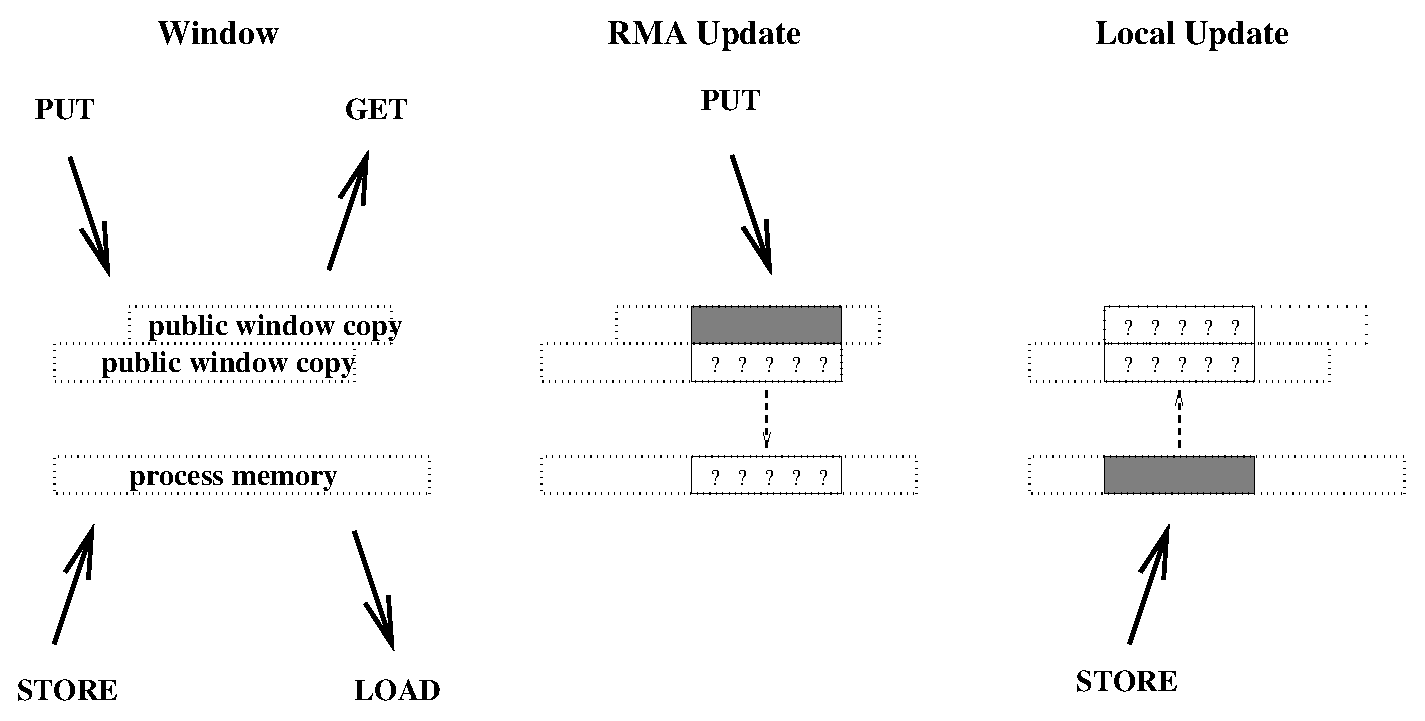
\includegraphics[width=6.0in]{figures/window1}}
% Rolf said this figure
% doesn't print well -- the content is also now well described in the text
% and somewhat confusing.  
\infloattrue
\caption{Schematic description of the public/private
window operations in the \mpiconst{MPI\_WIN\_SEPARATE} memory model for two
overlapping windows}
\label{fig:1sided-window}
\infloatfalse
\end{figure}

In the \RMA/ unified model, public and private copies are identical and
updates via put or accumulate operations are eventually observed by load accesses
without additional \RMA/ procedure calls. A store access to a window is eventually
visible to remote get or accumulate operations without additional \RMA/
procedure calls. These stronger semantics of the \RMA/ unified model allow the
user to omit some synchronization calls and potentially improve
performance.

\begin{users}
If accesses in the \RMA/ unified model are not synchronized (with locks or
flushes, see Section~\ref{sec:1sided-lock}), load/store accesses
might observe changes to the memory while they are in progress. The
order in which data is written is not specified unless further
synchronization is used.  This might lead to inconsistent views on
memory and programs that assume that a transfer is complete by only
checking parts of the message are erroneous.
\end{users}

The memory model for a particular \RMA/ window can be determined by
accessing the attribute \mpiconst{MPI\_WIN\_MODEL}.  If the memory model
is the unified model, the value of this attribute is
\mpiconstmain{MPI\_WIN\_UNIFIED}; otherwise, the value is
\mpiconstmain{MPI\_WIN\_SEPARATE}.

\section{Synchronization Calls}
\mpitermtitleindex{RMA@\RMA/!synchronization calls}
\mpitermtitleindex{synchronization calls!RMA@\RMA/}
\label{sec:1sided-sync}

\RMA/ communications fall in two categories:
\begin{description}
\item[\mpitermdef{active target communication},] where data is moved from the memory of one
\mpi/ process to the memory of another, and both are explicitly involved in the
communication.  This communication pattern is similar to message
passing, except that all the data transfer arguments are provided by
the origin process, and the target process only participates in the synchronization.
\item[\mpitermdef{passive target communication},] where data is moved from the memory of one
\mpi/ process to the memory of another, and only the origin process is
explicitly involved
in
the transfer.  Thus, two origin processes may communicate by accessing
the same location in a target window.  The \mpi/ process that owns the
target window may be distinct from the two communicating \mpi/ processes, 
in which case it does not participate explicitly in the communication.
This communication
paradigm is closest to a shared memory model, where shared data can be
accessed by all \mpi/ processes, irrespective 
of location.
\end{description}

\RMA/ communication calls with argument \mpiarg{win} must occur at an origin process
only within an \mpitermdef{access epoch} for \mpiarg{win}.  Such an epoch
is opened with an \RMA/ synchronization
call on \mpiarg{win}; it proceeds with zero or more \RMA/
communication calls (e.g., \mpifunc{MPI\_PUT}, \mpifunc{MPI\_GET} or
\mpifunc{MPI\_ACCUMULATE}) on \mpiarg{win}; it is closed with another
synchronization call on 
\mpiarg{win}. This allows users to amortize one synchronization with multiple data
transfers and provide implementors
more flexibility in the implementation of \RMA/ operations.

Distinct access epochs for \mpiarg{win} at the same \mpi/ process must be disjoint.
On the other hand, epochs pertaining to different \mpiarg{win} arguments
may
overlap.  Load/store accesses or other \MPI/ calls may also occur during
an epoch.

In active target communication, a target window can be accessed by \RMA/
operations only within an \mpitermdef{exposure epoch}. Such an epoch is
opened and closed by \RMA/ synchronization calls executed by the
target process.  Distinct exposure epochs at an \mpi/ process
on the same window must be disjoint, but such an exposure epoch
may overlap with exposure epochs on other windows or
with access epochs for the same or other window arguments.
There is a one-to-one matching between access epochs at origin
processes and exposure epochs on target processes:
\RMA/ operations issued by an origin process for a target window will
access that
target window during the same exposure epoch if and only if they were
issued during the same access 
epoch.

In passive target communication the target
process does not execute \RMA/ synchronization calls, and there is no
concept of an exposure 
epoch. 

\MPI/ provides three synchronization mechanisms:
\begin{enumerate}
\item
The
\mpifunc{MPI\_WIN\_FENCE} collective synchronization call supports a
simple synchronization pattern that is often used in parallel
computations: namely a loosely-synchronous model, where global
computation phases alternate with global communication phases.
This mechanism is most useful for loosely synchronous algorithms where
the graph of communicating \mpi/ processes changes very frequently, or where
each \mpi/ process communicates with many 
others.

This call is used for active target communication.  An access epoch at an
origin process or an exposure epoch at a target process is opened
and closed by calls to \mpifunc{MPI\_WIN\_FENCE}.  An origin process can
access windows at all target processes in the group of \mpiarg{win} during
such an access
epoch, and the local window can be accessed by all \mpi/ processes in the
group of \mpiarg{win} during such an exposure epoch.
\item
The four functions \mpifunc{MPI\_WIN\_START}, 
\mpifunc{MPI\_WIN\_COMPLETE},
\mpifuncshort{MPI\_WIN\_POST}, and
\mpifunc{MPI\_WIN\_WAIT} 
can be used to restrict synchronization to the minimum: only
pairs of communicating \mpi/ processes synchronize, and they do so only when
a synchronization is needed to order \RMA/ accesses to a
window correctly with respect to local accesses to that same window.
This mechanism may be 
more efficient when each \mpi/ process communicates with few (logical)
neighbors, and the communication graph is fixed or changes
infrequently.

These calls are used for 
active target communication.  An access epoch is opened
at the origin process
with a call to \mpifunc{MPI\_WIN\_START} and is closed by a call to
\mpifunc{MPI\_WIN\_COMPLETE}.  The start call has a group argument
that specifies the group of target processes for that
epoch. An exposure epoch is opened at the
target process by a call
to \mpifunc{MPI\_WIN\_POST} and is closed by a call to
\mpifunc{MPI\_WIN\_WAIT}.  The post call has a group argument that
specifies the set of origin processes for that 
epoch.
\item
Finally, \mpiterm{shared lock}
access is provided by the functions \mpifunc{MPI\_WIN\_LOCK},
\mpifunc{MPI\_WIN\_LOCK\_ALL}, \mpifunc{MPI\_WIN\_UNLOCK}, and
\mpifunc{MPI\_WIN\_UNLOCK\_ALL}.  \mpifunc{MPI\_WIN\_LOCK} and
\mpifunc{MPI\_WIN\_UNLOCK} also provide \mpiterm{exclusive lock} capability.
Lock synchronization
is useful for \MPI/ applications that
emulate a shared memory model via \MPI/ calls; e.g., in a ``bulletin board''
model, where \mpi/ processes can, at random times, access or update
different parts of the bulletin board.

These four calls provide passive target communication.  An access epoch is
opened by a call to \mpifunc{MPI\_WIN\_LOCK} or
\mpifunc{MPI\_WIN\_LOCK\_ALL} and closed by a call to
\mpifunc{MPI\_WIN\_UNLOCK} or \mpifunc{MPI\_WIN\_UNLOCK\_ALL}, respectively.  
\end{enumerate}

\begin{figure}[t]
\centerline{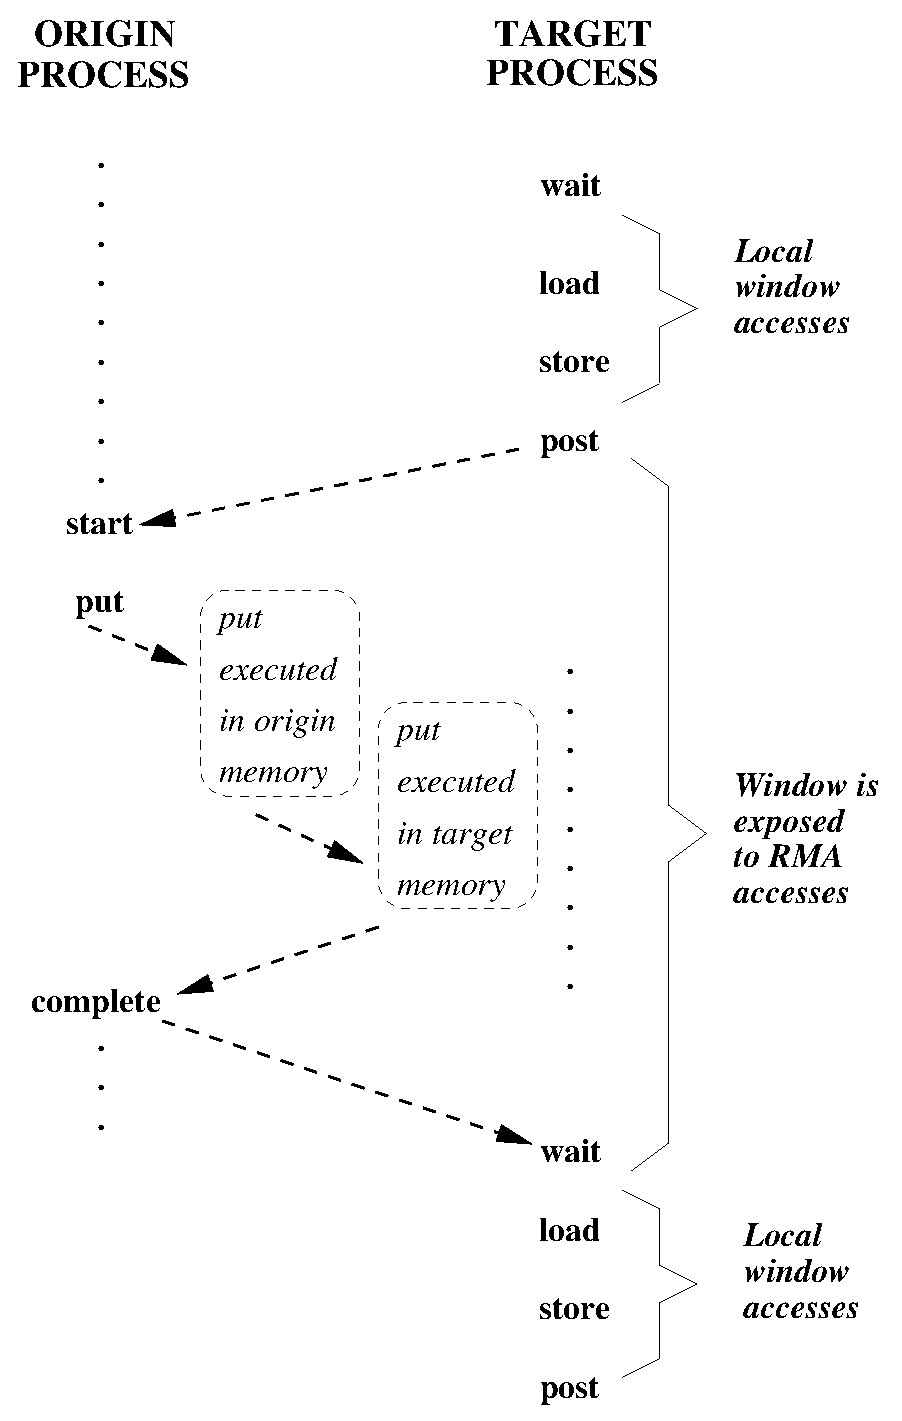
\includegraphics[width=3.0in]{figures/sync15}}
\caption[Active target communication]{Active target communication.  Dashed arrows represent
synchronizations (ordering of events).}
\label{fig:1sided-sync15}
\end{figure}

Figure~\ref{fig:1sided-sync15} illustrates the general synchronization
pattern for active target 
communication.
The synchronization between  \code{post} and
\code{start} ensures that the put operation of the origin process does
not start
until the target process exposes the window (with the \code{post} call);
the target process will
expose the window only after preceding local accesses to the window
have completed.
The synchronization between \code{complete} and \code{wait}
ensures that the put operation of the origin process completes at the origin and the target
before the window is unexposed (with the \code{wait} call).
The target process will execute
subsequent local accesses to the target window only after the \code{wait}
returned.

\begin{figure}[t]
\centerline{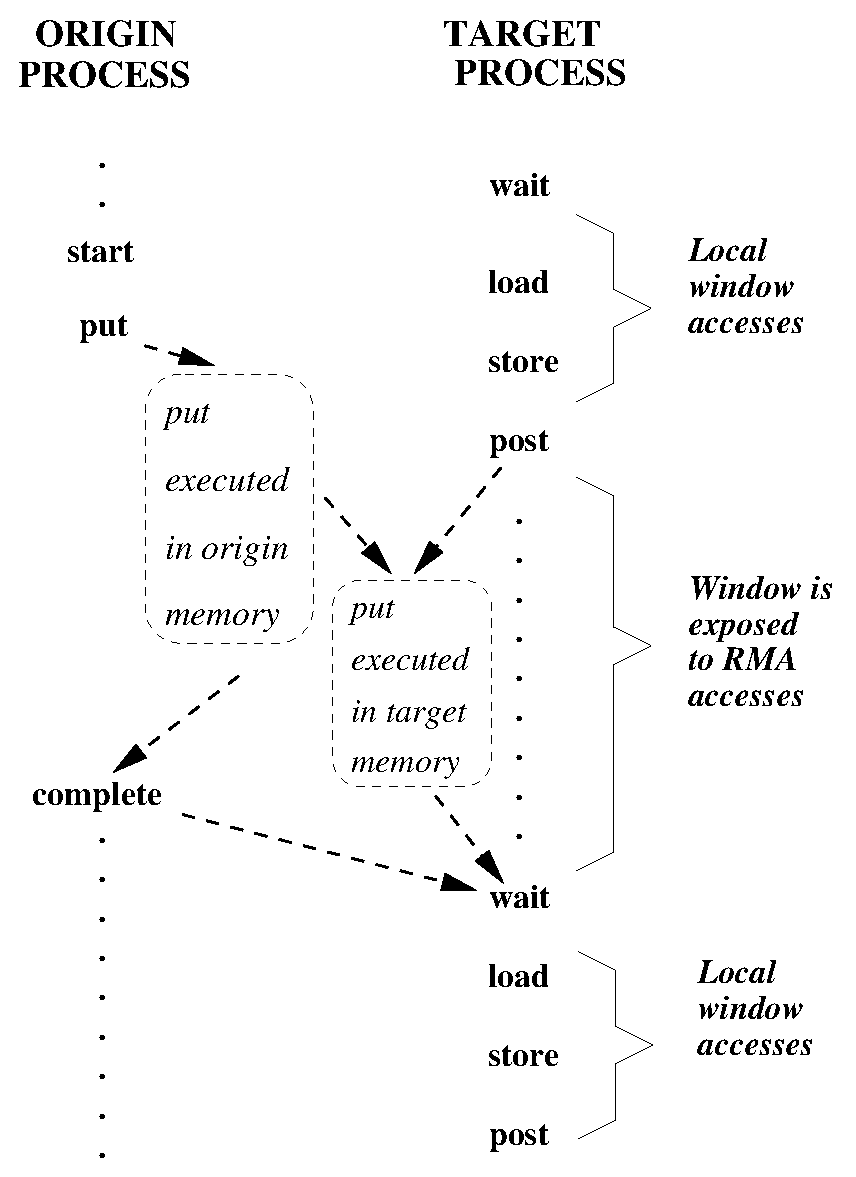
\includegraphics[width=3.0in]{figures/sync14}}
\caption[Active target communication, with weak synchronization]{Active target communication, with weak synchronization.  Dashed
arrows represent synchronizations (ordering of events).}
\label{fig:1sided-sync14}
\end{figure}

Figure~\ref{fig:1sided-sync15} shows operations occurring in the natural
temporal order implied by the synchronizations: the \code{post}
occurs before the matching \code{start}, and \code{complete} occurs before
the
matching \code{wait}.  However, such \mpitermdef{strong synchronization} is more
than
needed for correct ordering of window accesses.  The semantics of
\MPI/ calls allow \mpitermdef{weak synchronization}, 
as illustrated in Figure~\ref{fig:1sided-sync14}.
The access to the target window  is delayed until the window is
exposed, after the \code{post}. However the \code{start}
may return before the exposure epoch opens at the target. Similarly, the \code{put} and 
\code{complete} calls may also return before the exposure epoch opens at the target, if put data is
buffered by the implementation.
The synchronization calls correctly order window accesses, but do not
necessarily synchronize other operations.  This weaker synchronization
semantic allows for more efficient 
implementations.

\begin{figure}[t]
\centerline{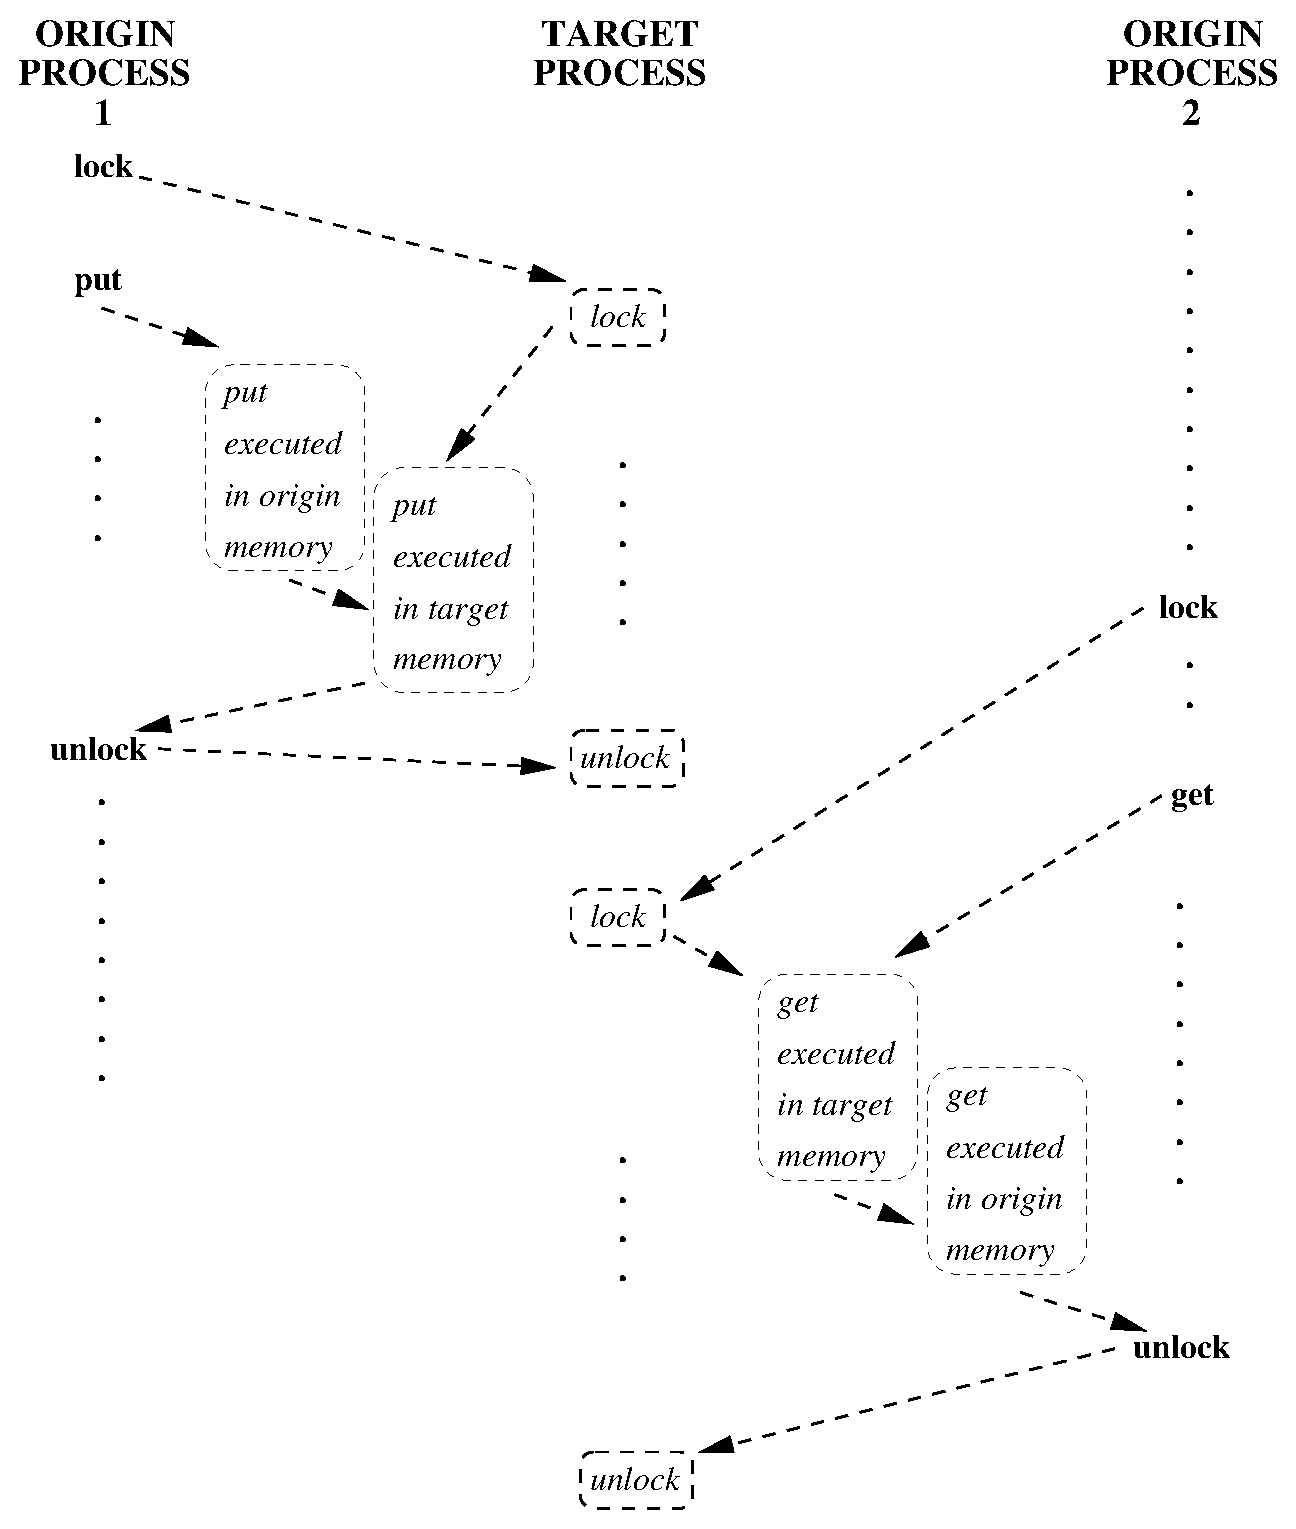
\includegraphics[width=4.5in]{figures/sync23}}
\caption[Passive target communication]{Passive target communication.  Dashed arrows represent
synchronizations (ordering of events).}
\label{fig:1sided-sync23}
\end{figure}

Figure~\ref{fig:1sided-sync23} illustrates the general synchronization
pattern for passive target 
communication.
The first origin process communicates data to the second
origin process, through the memory of the target process; the target
process is not explicitly involved in the 
communication.
The
\code{lock} and \code{unlock} calls ensure that the two \RMA/
accesses do not occur concurrently. However, they do \emph{not} ensure
that the \code{put} by origin 1 will precede the \code{get} by 
origin 2.

\begin{rationale}
\RMA/ does not define fine-grained mutexes in memory (only logical
coarse-grained window locks). \MPI/ provides the primitives (compare
and swap, accumulate, send/receive, etc.) needed to implement high-level
synchronization operations.
\end{rationale}

\subsection{Fence}

\cdeclindex{MPI\_Win}%
\begin{funcdef}{MPI\_WIN\_FENCE}{(\mbox{assert}, \mbox{win})}
\funcarg{\IN}{assert}{program assertion (integer)}
\funcarg{\IN}{win}{window object (handle)}
\end{funcdef}
\mpibindmain{MPI\_Win\_fence}{(\gb{}int~assert, MPI\_Win~win)}
\mpifnewbindmain{MPI\_Win\_fence}{(assert, win, ierror) \fargs INTEGER, INTENT(IN)\ ::\ \mbox{assert}\fnarg{}TYPE(MPI\_Win), INTENT(IN)\ ::\ \mbox{win}\fnfinalarg{}INTEGER, OPTIONAL, INTENT(OUT)\ ::\ \mbox{ierror}}
\mpifbindmain{MPI\_WIN\_FENCE}{(ASSERT, WIN, IERROR) \fargs \fnfinalarg{}INTEGER \mbox{ASSERT}, \mbox{WIN}, \mbox{IERROR}}

\mpifunc{MPI\_WIN\_FENCE} synchronizes
\RMA/ communication operations on \mpiargshort{win}.  The procedure is collective over the group of
\mpiargshort{win}.
All \RMA/
operations on \mpiargshort{win} originating at a given origin process and started
before the fence call will complete at that \mpi/ process
before the fence call returns.  
They will be completed at their target before the fence
call returns at the target.
Store accesses to shared-memory of \mpiargshort{win} will become visible
before the fence call returns at the target.
\RMA/ operations on \mpiargshort{win} started by
an origin process after the fence call returns will access their target
window only after \mpifunc{MPI\_WIN\_FENCE} has been
called by the target process.

The call closes an \RMA/ access epoch if it was preceded by
another fence call and the local \mpi/ process initiated any \RMA/ communication
operations on \mpiarg{win} between these two calls.  The call
closes an \RMA/ exposure epoch if it was
preceded by another fence call and the local window was the target of \RMA/
accesses between these two calls.  The call opens an
\RMA/ access epoch if it is followed by another fence call and by
\RMA/ communication calls issued between these two fence calls.  The
call opens an exposure epoch if it is followed by another fence call
and the local window is the target of \RMA/ accesses between these two fence calls.
Thus, the fence call is equivalent to calls to a subset of
\code{post}, \code{start}, \code{complete}, \code{wait}.

A call to \mpifunc{MPI\_WIN\_FENCE} is usually synchronizing.
However, a call to \mpifunc{MPI\_WIN\_FENCE}
that is known not to close any epoch
(in particular, a call with the \mpiconst{MPI\_MODE\_NOPRECEDE} \mpiarg{assert} set) is
not necessarily synchronizing.

The \mpiarg{assert} argument is used to provide assertions on the
context of the call that may be used for various optimizations.  This
is described in
Section~\ref{sec:1sided-assert}.  A value of \mpiarg{assert}\mpicode{ = 0} is
always valid.

\begin{users}
Calls to \mpifunc{MPI\_WIN\_FENCE} should both precede and follow calls to
\RMA/ communication procedures that are synchronized with fence calls.
\end{users}

\subsection{General Active Target Synchronization}
\label{sec:1sided-pscw}
\label{sec:1sided-sync:pscw}

\cdeclindex{MPI\_Group}%
\cdeclindex{MPI\_Win}%
\begin{funcdef}{MPI\_WIN\_START}{(\mbox{group}, \mbox{assert}, \mbox{win})}
\funcarg{\IN}{group}{group of target processes (handle)}
\funcarg{\IN}{assert}{program assertion (integer)}
\funcarg{\IN}{win}{window object (handle)}
\end{funcdef}
\mpibindmain{MPI\_Win\_start}{(\gb{}MPI\_Group~group, int~assert, MPI\_Win~win)}
\mpifnewbindmain{MPI\_Win\_start}{(group, assert, win, ierror) \fargs TYPE(MPI\_Group), INTENT(IN)\ ::\ \mbox{group}\fnarg{}INTEGER, INTENT(IN)\ ::\ \mbox{assert}\fnarg{}TYPE(MPI\_Win), INTENT(IN)\ ::\ \mbox{win}\fnfinalarg{}INTEGER, OPTIONAL, INTENT(OUT)\ ::\ \mbox{ierror}}
\mpifbindmain{MPI\_WIN\_START}{(GROUP, ASSERT, WIN, IERROR) \fargs \fnfinalarg{}INTEGER \mbox{GROUP}, \mbox{ASSERT}, \mbox{WIN}, \mbox{IERROR}}

Opens an \RMA/ access epoch for \mpiarg{win}.  \RMA/ calls issued on
\mpiarg{win} during this epoch must access only windows at
\mpi/ processes in \mpiarg{group}.
Each \mpi/ process in \mpiarg{group} must issue a matching call to 
\mpifunc{MPI\_WIN\_POST}.
\RMA/ accesses to each target
window will be delayed, if necessary,
until the target process executed the matching call to 
\mpifunc{MPI\_WIN\_POST}.
\mpifunc{MPI\_WIN\_START} is allowed to delay its return until the corresponding calls to
\mpifunc{MPI\_WIN\_POST} have occurred, but is not required to.

The \mpiarg{assert} argument is used to provide assertions on the
context of the call that may be used for various optimizations.  This
is described in
Section~\ref{sec:1sided-assert}.  A value of \mpiarg{assert}\mpicode{ = 0} is
always valid.

\cdeclindex{MPI\_Win}%
\begin{funcdef}{MPI\_WIN\_COMPLETE}{(\mbox{win})}
\funcarg{\IN}{win}{window object (handle)}
\end{funcdef}
\mpibindmain{MPI\_Win\_complete}{(\gb{}MPI\_Win~win)}
\mpifnewbindmain{MPI\_Win\_complete}{(win, ierror) \fargs TYPE(MPI\_Win), INTENT(IN)\ ::\ \mbox{win}\fnfinalarg{}INTEGER, OPTIONAL, INTENT(OUT)\ ::\ \mbox{ierror}}
\mpifbindmain{MPI\_WIN\_COMPLETE}{(WIN, IERROR) \fargs \fnfinalarg{}INTEGER \mbox{WIN}, \mbox{IERROR}}

Closes an \RMA/ access epoch on \mpiarg{win} opened by a
call to \mpifunc{MPI\_WIN\_START}.  All \RMA/ communication
operations initiated on \mpiarg{win} during this epoch will have completed at
the origin when the call returns.
All updates to shared memory in \mpiarg{win} through load/store accesses executed during this epoch will be visible
at the target when the call returns.

\mpifunc{MPI\_WIN\_COMPLETE} enforces completion of preceding \RMA/
operations and visibility of load/store accesses at the origin, but not at the target.
A put or accumulate operation may not have completed
at the target when it has completed at the origin.

Consider the sequence of calls in the example below.
\begin{example}
\label{ex:1sided-start-complete}
\Exindex[\RMA/ Start and complete]{C}{RMA Start and complete@\RMA/ Start and complete}{MPI\_Win\_start,MPI\_Put,MPI\_Win\_complete}%
Use of \mpifunc{MPI\_WIN\_START} and \mpifunc{MPI\_WIN\_COMPLETE}.
%%HEADER
%%SKIP
%%ENDHEADER
\begin{lstlisting}[language={[MPI]C}]
MPI_Win_start(group, flag, win);
MPI_Put(..., win);
MPI_Win_complete(win);
\end{lstlisting}

The call to \mpifunc{MPI\_WIN\_COMPLETE} does not return until the
put operation has completed at the origin; and
the target window will be accessed by the put operation only after the
call to \mpifunc{MPI\_WIN\_START} has matched a call to
\mpifunc{MPI\_WIN\_POST} by the target process.
\end{example}

\begin{implementors}
The semantics described above still leave
much choice to implementors. The return from the call to
\mpifunc{MPI\_WIN\_START} can block until the matching call to
\mpifunc{MPI\_WIN\_POST} occurs at all target processes.  One can also
have implementations where the call to \mpifunc{MPI\_WIN\_START} returns immediately, but the
call to \mpifunc{MPI\_WIN\_COMPLETE} delays its return until the call to
\mpifunc{MPI\_WIN\_POST} occurred; or implementations where all
three calls can complete before any target process
has called 
\mpifunc{MPI\_WIN\_POST}---the
data put must be buffered, in this last case, so as to allow the
put to complete at the origin ahead of its completion at the 
target.
However, once the
call to \mpifunc{MPI\_WIN\_POST} is issued, the sequence above
must complete, without further dependencies.
\end{implementors}

\begin{users}
In order to ensure a portable deadlock free program, users must assume that
\mpifunc{MPI\_WIN\_START} may delay its return until the corresponding call
to \mpifunc{MPI\_WIN\_POST} has occurred.
\end{users}

\cdeclindex{MPI\_Group}%
\cdeclindex{MPI\_Win}%
\begin{funcdef}{MPI\_WIN\_POST}{(\mbox{group}, \mbox{assert}, \mbox{win})}
\funcarg{\IN}{group}{group of origin processes (handle)}
\funcarg{\IN}{assert}{program assertion (integer)}
\funcarg{\IN}{win}{window object (handle)}
\end{funcdef}
\mpibindmain{MPI\_Win\_post}{(\gb{}MPI\_Group~group, int~assert, MPI\_Win~win)}
\mpifnewbindmain{MPI\_Win\_post}{(group, assert, win, ierror) \fargs TYPE(MPI\_Group), INTENT(IN)\ ::\ \mbox{group}\fnarg{}INTEGER, INTENT(IN)\ ::\ \mbox{assert}\fnarg{}TYPE(MPI\_Win), INTENT(IN)\ ::\ \mbox{win}\fnfinalarg{}INTEGER, OPTIONAL, INTENT(OUT)\ ::\ \mbox{ierror}}
\mpifbindmain{MPI\_WIN\_POST}{(GROUP, ASSERT, WIN, IERROR) \fargs \fnfinalarg{}INTEGER \mbox{GROUP}, \mbox{ASSERT}, \mbox{WIN}, \mbox{IERROR}}

Opens an \RMA/ exposure epoch for the
local window associated with \mpiarg{win}.  Only \mpi/ processes in
\mpiarg{group} may access the window with \RMA/ calls on
\mpiarg{win} during  this 
epoch.
Each \mpi/ process in \mpiarg{group} must issue a matching call to 
\mpifunc{MPI\_WIN\_START}.
\mpifunc{MPI\_WIN\_POST} is a \mpiterm{local} procedure.

\cdeclindex{MPI\_Win}%
\begin{funcdef}{MPI\_WIN\_WAIT}{(\mbox{win})}
\funcarg{\IN}{win}{window object (handle)}
\end{funcdef}
\mpibindmain{MPI\_Win\_wait}{(\gb{}MPI\_Win~win)}
\mpifnewbindmain{MPI\_Win\_wait}{(win, ierror) \fargs TYPE(MPI\_Win), INTENT(IN)\ ::\ \mbox{win}\fnfinalarg{}INTEGER, OPTIONAL, INTENT(OUT)\ ::\ \mbox{ierror}}
\mpifbindmain{MPI\_WIN\_WAIT}{(WIN, IERROR) \fargs \fnfinalarg{}INTEGER \mbox{WIN}, \mbox{IERROR}}

Closes an \RMA/ exposure epoch opened by a call to
\mpifunc{MPI\_WIN\_POST} on 
\mpiarg{win}.
This call matches calls to \mpifunc{MPI\_WIN\_COMPLETE} on \mpiarg{win}
issued
by each of the origin processes that were granted access to the window
during this epoch.
The call to \mpifunc{MPI\_WIN\_WAIT} will
return only after all matching calls to \mpifunc{MPI\_WIN\_COMPLETE}
have occurred.
This guarantees that all these origin processes have completed their
\RMA/ operations and shared-memory load/store accesses have become visible on the local
window.
When the call returns, all these \RMA/ accesses will
have completed at the target window.

Figure~\ref{fig:1sided-2party} illustrates the use of these four
functions.
\begin{figure}
\centerline{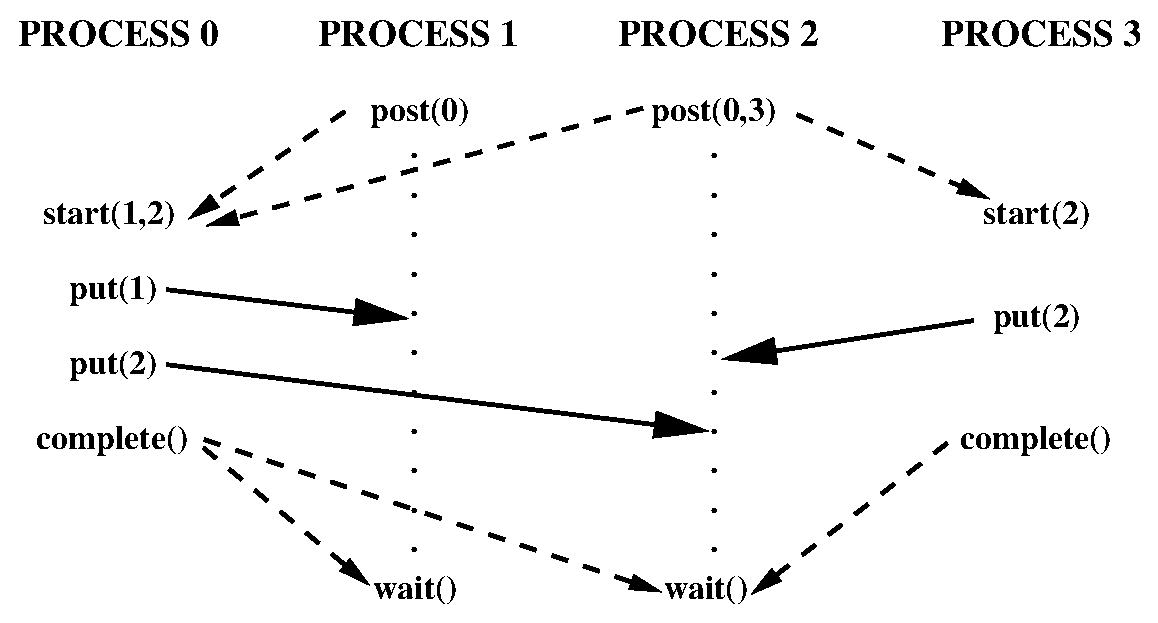
\includegraphics[width=4.5in]{figures/2party}}
\caption[Active target communication with several \mpi/ processes and strong synchronization]{Active target communication, with strong synchronization.  Dashed arrows represent
synchronizations and solid arrows represent data transfer.}
\label{fig:1sided-2party}
\end{figure}
Process~0 puts data in the windows of processes~1 and~2 and process~3
puts data in the window of process~2.  Each start call lists the ranks
of the \mpi/ processes whose windows will be accessed;
each post call lists the ranks of the
\mpi/ processes that access the local window.  The figure illustrates a
possible timing for the events, assuming strong synchronization; in a 
weak synchronization, the start, put or complete calls
may occur ahead of the matching post calls.

\cdeclindex{MPI\_Win}%
\begin{funcdef}{MPI\_WIN\_TEST}{(\mbox{win}, \mbox{flag})}
\funcarg{\IN}{win}{window object (handle)}
\funcarg{\OUT}{flag}{success flag (logical)}
\end{funcdef}
\mpibindmain{MPI\_Win\_test}{(\gb{}MPI\_Win~win, int~*flag)}
\mpifnewbindmain{MPI\_Win\_test}{(win, flag, ierror) \fargs TYPE(MPI\_Win), INTENT(IN)\ ::\ \mbox{win}\fnarg{}LOGICAL, INTENT(OUT)\ ::\ \mbox{flag}\fnfinalarg{}INTEGER, OPTIONAL, INTENT(OUT)\ ::\ \mbox{ierror}}
\mpifbindmain{MPI\_WIN\_TEST}{(WIN, FLAG, IERROR) \fargs INTEGER \mbox{WIN}, \mbox{IERROR}\fnfinalarg{}LOGICAL \mbox{FLAG}}

\mpifunc{MPI\_WIN\_TEST} is a local procedure.
Repeated calls to \mpifunc{MPI\_WIN\_TEST} with the same \mpiarg{win} argument
will eventually return \mpiarg{flag}\code{ = true} once all accesses to the
local window by the group to which it was exposed by the corresponding call to
\mpifunc{MPI\_WIN\_POST} have been completed as indicated by matching
\mpifunc{MPI\_WIN\_COMPLETE} calls, and \mpiarg{flag}\code{ = false} otherwise.
In the former case \mpifunc{MPI\_WIN\_WAIT}
would have returned immediately.
The effect of return of \mpifunc{MPI\_WIN\_TEST} with
\mpiarg{flag}\mpicode{ = true} is the same as the effect of a return 
of \mpifunc{MPI\_WIN\_WAIT}.  If \mpiarg{flag}\mpicode{ = false} is returned,
then the call has no visible effect.

\mpifunc{MPI\_WIN\_TEST} should be called only where
\mpifunc{MPI\_WIN\_WAIT}
can be called.
Once the call has returned \mpiarg{flag}\mpicode{ = true}, it must not be
called again, until the window is posted again.

Assume that window \mpiarg{win} is associated with a ``hidden''\mpitermtitleindex{communicator!hidden} 
communicator \mpicode{wincomm}, used for communication by the \mpi/ processes
in the group of \mpiarg{win}.  The rules for matching of post and start calls and
for matching complete and wait calls can be
derived from the rules for 
matching sends and receives, by considering the following (partial) model
implementation. 

\begin{description}
\item[\mpifunc{MPI\_WIN\_POST}\mpicode{(group,0,win)}]
initiates a nonblocking send with tag \mpicode{tag0} to each
\mpi/ process in \mpiarg{group}, using \mpicode{wincomm}.
\item[\mpifunc{MPI\_WIN\_START}\mpicode{(group,0,win)}]
initiates a nonblocking receive with tag \mpicode{tag0} from each \mpi/
process in \mpiarg{group}, using \mpicode{wincomm}.  An \RMA/ access to
a target process is delayed until the receive
from that \mpi/ process is completed.
\item[\mpifunc{MPI\_WIN\_COMPLETE}\mpicode{(win)}]
initiates a nonblocking send with tag \mpicode{tag1} to each \mpi/ process in
the group of the preceding start call.
\item[\mpifunc{MPI\_WIN\_WAIT}\mpicode{(win)}]
initiates a nonblocking receive with tag \mpicode{tag1} from each
\mpi/ process in the group of the preceding post call.  Wait for the
completion of all receives. 
\end{description}

No races can occur in a correct program: each of the sends matches a
unique receive, and vice versa. 

\begin{rationale}
The design for general active target synchronization requires the
user to provide complete information on the communication pattern, at
each end of a communication link: each origin specifies a list of
targets, and each target specifies a list of origins.  This provides
maximum flexibility (hence, efficiency) for the implementor: 
each
synchronization can be initiated by either side, since each ``knows''
the identity of the other.  This also provides maximum protection from
possible races.  On the other hand, the design requires more
information than \RMA/ needs: in general, it is sufficient
for the origin to know the rank of the target, but not vice
versa.
Users that want more ``anonymous'' communication will be required to
use the fence or lock mechanisms.
\end{rationale}

\begin{users}
Assume a communication pattern that is represented by a directed graph
$G = \langle V, E\rangle$, where $V = \{0, \ldots, n-1\}$ and $ij \in E$ if origin process
$i$ accesses the window at target process $j$.  Then each \mpi/ process $i$
issues a call to 
\mpifunc{MPI\_WIN\_POST}\mpicode{($ingroup_i$, \ldots)}, 
followed by a call to\flushline
\mpifunc{MPI\_WIN\_START}\mpicode{($outgroup_i$,\ldots)},
where 
$outgroup_i = \{ j ~:~ ij \in E\}$ and $ingroup_i = \{ j ~:~ ji \in E
\}$.  A call is a no-op, and can be skipped, if the \mpiarg{group} argument is
empty. After the communications calls, each \mpi/ process that issued
a start will issue a complete.  Finally, each \mpi/ process that
issued  a post will issue a wait. 

Note that each \mpi/ process may call with a \mpiarg{group} argument that has
different members.
\end{users}
  
\subsection{Lock}
\label{sec:1sided-lock}

Locks are used to protect accesses to the locked target
window effected by \RMA/ calls issued between the lock and unlock
calls, and to protect
load/store accesses to a locked local or shared
memory window executed between the lock and unlock
calls.
Accesses that are protected by an \mpitermdef{exclusive lock} (acquired using \mpiconstmain{MPI\_LOCK\_EXCLUSIVE})
will not be concurrent at the window site
with other accesses to the same window that are lock protected.
Accesses that are protected by a \mpitermdef{shared lock} (acquired using \mpiconstmain{MPI\_LOCK\_SHARED}) will not be
concurrent at the window site with
accesses protected by an exclusive lock to the same window.

\cdeclindex{MPI\_Win}%
\begin{funcdef}{MPI\_WIN\_LOCK}{(\mbox{lock\_type}, \mbox{rank}, \mbox{assert}, \mbox{win})}
\funcarg{\IN}{lock\_type}{either \mpiconst{MPI\_LOCK\_EXCLUSIVE} or \mpiconst{MPI\_LOCK\_SHARED} (state)}
\funcarg{\IN}{rank}{rank of target \MPI/ process in the group of the window \mpiarg{win} (nonnegative integer)}
\funcarg{\IN}{assert}{program assertion (integer)}
\funcarg{\IN}{win}{window object (handle)}
\end{funcdef}
\mpibindmain{MPI\_Win\_lock}{(\gb{}int~lock\_type, int~rank, int~assert, MPI\_Win~win)}
\mpifnewbindmain{MPI\_Win\_lock}{(lock\_type, rank, assert, win, ierror) \fargs INTEGER, INTENT(IN)\ ::\ \mbox{lock\_type}, \mbox{rank}, \mbox{assert}\fnarg{}TYPE(MPI\_Win), INTENT(IN)\ ::\ \mbox{win}\fnfinalarg{}INTEGER, OPTIONAL, INTENT(OUT)\ ::\ \mbox{ierror}}
\mpifbindmain{MPI\_WIN\_LOCK}{(LOCK\_TYPE, RANK, ASSERT, WIN, IERROR) \fargs \fnfinalarg{}INTEGER \mbox{LOCK\_TYPE}, \mbox{RANK}, \mbox{ASSERT}, \mbox{WIN}, \mbox{IERROR}}

Opens an \RMA/ access epoch.
The
window at the
\mpi/ process with a rank of \mpiarg{rank} in the group of \mpiarg{win} can be accessed by \RMA/ operations
on \mpiarg{win} during that
epoch.
Multiple \RMA/ access epochs (with calls to \mpifunc{MPI\_WIN\_LOCK})
can occur simultaneously; however, each access epoch must target a
different \mpi/ process.

\cdeclindex{MPI\_Win}%
\begin{funcdef}{MPI\_WIN\_LOCK\_ALL}{(\mbox{assert}, \mbox{win})}
\funcarg{\IN}{assert}{program assertion (integer)}
\funcarg{\IN}{win}{window object (handle)}
\end{funcdef}
\mpibindmain{MPI\_Win\_lock\_all}{(\gb{}int~assert, MPI\_Win~win)}
\mpifnewbindmain{MPI\_Win\_lock\_all}{(assert, win, ierror) \fargs INTEGER, INTENT(IN)\ ::\ \mbox{assert}\fnarg{}TYPE(MPI\_Win), INTENT(IN)\ ::\ \mbox{win}\fnfinalarg{}INTEGER, OPTIONAL, INTENT(OUT)\ ::\ \mbox{ierror}}
\mpifbindmain{MPI\_WIN\_LOCK\_ALL}{(ASSERT, WIN, IERROR) \fargs \fnfinalarg{}INTEGER \mbox{ASSERT}, \mbox{WIN}, \mbox{IERROR}}

Opens an \RMA/ access epoch to all \mpi/ processes in
\mpiarg{win}, with a lock type of \mpiconst{MPI\_LOCK\_SHARED}. 
During the epoch, the calling \mpi/ process can access the window memory on all
\mpi/ processes in \mpiarg{win} by using \RMA/ operations. A window locked with
\mpifunc{MPI\_WIN\_LOCK\_ALL} must be unlocked with
\mpifunc{MPI\_WIN\_UNLOCK\_ALL}.  This routine is not collective---the
\mpiarg{ALL} refers to a lock on all members of the group of the window.

\begin{users}
There may be additional overheads associated with using
\mpifunc{MPI\_WIN\_LOCK} and \mpifunc{MPI\_WIN\_LOCK\_ALL} concurrently
on the same window. These overheads could be avoided by specifying the
assertion \mpiconst{MPI\_MODE\_NOCHECK} when possible (see
Section~\ref{sec:1sided-assert}).
\end{users}

\cdeclindex{MPI\_Win}%
\begin{funcdef}{MPI\_WIN\_UNLOCK}{(\mbox{rank}, \mbox{win})}
\funcarg{\IN}{rank}{rank of target \MPI/ process in the group of the window \mpiarg{win} (nonnegative integer)}
\funcarg{\IN}{win}{window object (handle)}
\end{funcdef}
\mpibindmain{MPI\_Win\_unlock}{(\gb{}int~rank, MPI\_Win~win)}
\mpifnewbindmain{MPI\_Win\_unlock}{(rank, win, ierror) \fargs INTEGER, INTENT(IN)\ ::\ \mbox{rank}\fnarg{}TYPE(MPI\_Win), INTENT(IN)\ ::\ \mbox{win}\fnfinalarg{}INTEGER, OPTIONAL, INTENT(OUT)\ ::\ \mbox{ierror}}
\mpifbindmain{MPI\_WIN\_UNLOCK}{(RANK, WIN, IERROR) \fargs \fnfinalarg{}INTEGER \mbox{RANK}, \mbox{WIN}, \mbox{IERROR}}

Closes an \RMA/ access epoch opened by a call to
\mpifunc{MPI\_WIN\_LOCK} on window \mpiarg{win}.
\RMA/ operations issued during this
period will have completed both at the origin and at the target when the call returns.

\cdeclindex{MPI\_Win}%
\begin{funcdef}{MPI\_WIN\_UNLOCK\_ALL}{(\mbox{win})}
\funcarg{\IN}{win}{window object (handle)}
\end{funcdef}
\mpibindmain{MPI\_Win\_unlock\_all}{(\gb{}MPI\_Win~win)}
\mpifnewbindmain{MPI\_Win\_unlock\_all}{(win, ierror) \fargs TYPE(MPI\_Win), INTENT(IN)\ ::\ \mbox{win}\fnfinalarg{}INTEGER, OPTIONAL, INTENT(OUT)\ ::\ \mbox{ierror}}
\mpifbindmain{MPI\_WIN\_UNLOCK\_ALL}{(WIN, IERROR) \fargs \fnfinalarg{}INTEGER \mbox{WIN}, \mbox{IERROR}}

Closes a shared \RMA/ access epoch opened by a call to
\mpifunc{MPI\_WIN\_LOCK\_ALL} on window \mpiarg{win}.
\RMA/ operations issued during this
epoch will have completed both at the origin and at the target when the call returns.

\bigskip%%ALLOWLATEX%%

It is erroneous to have a window locked and exposed (in an exposure
epoch) concurrently.  For example, an \mpi/ process may not call
\mpifunc{MPI\_WIN\_LOCK} to lock a target window if the target process
has called \mpifunc{MPI\_WIN\_POST} and has not yet called
\mpifunc{MPI\_WIN\_WAIT}; it is erroneous to call
\mpifunc{MPI\_WIN\_POST} while the local window is locked.

\begin{rationale}
An alternative is to require \MPI/ to enforce mutual exclusion between exposure epochs and locking periods.  However, this would entail additional
overheads when locks or active target synchronization do not interact
in support of those rare interactions between the two mechanisms.  The
programming style that we encourage here is that a set of windows is
used with only one synchronization mechanism at a time, with shifts
from one mechanism to another being rare and involving global synchronization.
\end{rationale}

\begin{users}
Users need to use explicit synchronization code in order to enforce
mutual exclusion between locking periods and exposure epochs on a
window.
\end{users}

%
% WDG notes:
% These two sentances say different things.  Not just the locks, but the use
% of \RMA/ synchronized by locks, can only be done portably in memory acquired
% through ALLOC_MEM.  The text is correct but misleading.
%
Implementors may restrict the use of \RMA/ communication that is 
synchronized by lock calls to windows in memory allocated by 
\mpifunc{MPI\_ALLOC\_MEM} 
(\sectionref{sec:misc-memalloc}),
\mpifunc{MPI\_WIN\_ALLOCATE} (\sectionref{sec:winalloc}),
\mpifunc{MPI\_WIN\_ALLOCATE\_SHARED} (\sectionref{sec:winallocshared}), or attached with
\mpifunc{MPI\_WIN\_ATTACH} \gb(\sectionref{sec:rma-create-dynamic}).
Locks can be used portably only in such memory.

\begin{rationale}
The implementation of passive target communication between processes in different \mpitermni{shared memory domains}\mpitermindex{shared memory!domain}
may require an asynchronous software 
agent.  Such an agent can be implemented more easily, and can achieve
better performance, if restricted to specially allocated memory.  It
can be avoided altogether if \mpiterm{shared memory} is used. It seems natural to
impose restrictions that allow the use of shared memory for
\RMA/ communication in shared memory machines.

%% B3.1
%The downside of this decision is that passive target communication cannot be
%used without taking advantage of nonstandard Fortran features: namely,
%the availability of C-like pointers; these are not supported by some
%Fortran
%compilers.
%% E3.1
\end{rationale}

Consider the sequence of calls in the example below.
\begin{example}
\label{ex:1sided-lock-unlock}%
\Exindex[\RMA/ Lock and unlock]{C}{RMA Lock and unlock@\RMA/ Lock and unlock}{MPI\_Win\_lock,MPI\_Put,MPI\_Win\_unlock}%
Use of \mpifunc{MPI\_WIN\_LOCK} and \mpifunc{MPI\_WIN\_UNLOCK}.
%%HEADER
%%LANG: C
%%FRAGMENT
%%DECL: MPI_Win win; int rank; int buf; MPI_Aint todisp; int assert;
%%SUBST:\.\.\., r:&buf,1,MPI_INT, r
%%SUBST:\.\.\., w:todisp,1,MPI_INT, w
%%ENDHEADER
\begin{lstlisting}[language={[MPI]C}]
MPI_Win_lock(MPI_LOCK_EXCLUSIVE, rank, assert, win);
MPI_Put(..., rank, ..., win);
MPI_Win_unlock(rank, win);
\end{lstlisting}
The call to \mpifunc{MPI\_WIN\_UNLOCK} will not return until the put
transfer has completed at the origin
and at the target.
\end{example}

\begin{implementors}
The semantics described above still leave much freedom to implementors.
Return from the call to
\mpifunc{MPI\_WIN\_LOCK} may be delayed until an
exclusive lock on the window is acquired; or, the first
two calls may return immediately, while return from \mpifunc{MPI\_WIN\_UNLOCK} is delayed until
a lock is acquired---the update of the target window is then
postponed until the call to \mpifunc{MPI\_WIN\_UNLOCK} occurs.
However,  if the call to \mpifunc{MPI\_WIN\_LOCK} is used to lock a
window accessible via load/store accesses (i.e., a local window or a window at an \MPI/ process
for which a pointer to shared memory can be obtained via \mpifunc{MPI\_WIN\_SHARED\_QUERY}),
then the call must not return before the lock is acquired,
since the lock may protect load/store accesses to the window issued
after the lock call returns.
\end{implementors}

\begin{users}
In order to ensure a portable deadlock free program, a user must assume
that \mpifunc{MPI\_WIN\_LOCK} may delay its return until the desired lock on the
window has been acquired.
\end{users}

\subsection{Flush and Sync}
\label{sec:1sided-flush}

All flush and sync functions can be called only within passive target
epochs.

\cdeclindex{MPI\_Win}%
\begin{funcdef}{MPI\_WIN\_FLUSH}{(\mbox{rank}, \mbox{win})}
\funcarg{\IN}{rank}{rank of target \MPI/ process in the group of the window \mpiarg{win} (nonnegative integer)}
\funcarg{\IN}{win}{window object (handle)}
\end{funcdef}
\mpibindmain{MPI\_Win\_flush}{(\gb{}int~rank, MPI\_Win~win)}
\mpifnewbindmain{MPI\_Win\_flush}{(rank, win, ierror) \fargs INTEGER, INTENT(IN)\ ::\ \mbox{rank}\fnarg{}TYPE(MPI\_Win), INTENT(IN)\ ::\ \mbox{win}\fnfinalarg{}INTEGER, OPTIONAL, INTENT(OUT)\ ::\ \mbox{ierror}}
\mpifbindmain{MPI\_WIN\_FLUSH}{(RANK, WIN, IERROR) \fargs \fnfinalarg{}INTEGER \mbox{RANK}, \mbox{WIN}, \mbox{IERROR}}

All outstanding \RMA/ operations on \mpiarg{win} initiated by
the \mpi/ process calling this procedure to the target with \mpiarg{rank} in the group of the specified window
will have completed when \mpifunc{MPI\_WIN\_FLUSH} returns. The operations are completed both at
the origin and at the target. 

\cdeclindex{MPI\_Win}%
\begin{funcdef}{MPI\_WIN\_FLUSH\_ALL}{(\mbox{win})}
\funcarg{\IN}{win}{window object (handle)}
\end{funcdef}
\mpibindmain{MPI\_Win\_flush\_all}{(\gb{}MPI\_Win~win)}
\mpifnewbindmain{MPI\_Win\_flush\_all}{(win, ierror) \fargs TYPE(MPI\_Win), INTENT(IN)\ ::\ \mbox{win}\fnfinalarg{}INTEGER, OPTIONAL, INTENT(OUT)\ ::\ \mbox{ierror}}
\mpifbindmain{MPI\_WIN\_FLUSH\_ALL}{(WIN, IERROR) \fargs \fnfinalarg{}INTEGER \mbox{WIN}, \mbox{IERROR}}

All \RMA/ operations initiated by the \MPI/ process calling this procedure to any target on the specified window
prior to this call will have
completed both at the origin and at the target when \mpifunc{MPI\_WIN\_FLUSH\_ALL}
returns. 

\cdeclindex{MPI\_Win}%
\begin{funcdef}{MPI\_WIN\_FLUSH\_LOCAL}{(\mbox{rank}, \mbox{win})}
\funcarg{\IN}{rank}{rank of target \MPI/ process in the group of the window \mpiarg{win} (nonnegative integer)}
\funcarg{\IN}{win}{window object (handle)}
\end{funcdef}
\mpibindmain{MPI\_Win\_flush\_local}{(\gb{}int~rank, MPI\_Win~win)}
\mpifnewbindmain{MPI\_Win\_flush\_local}{(rank, win, ierror) \fargs INTEGER, INTENT(IN)\ ::\ \mbox{rank}\fnarg{}TYPE(MPI\_Win), INTENT(IN)\ ::\ \mbox{win}\fnfinalarg{}INTEGER, OPTIONAL, INTENT(OUT)\ ::\ \mbox{ierror}}
\mpifbindmain{MPI\_WIN\_FLUSH\_LOCAL}{(RANK, WIN, IERROR) \fargs \fnfinalarg{}INTEGER \mbox{RANK}, \mbox{WIN}, \mbox{IERROR}}

All outstanding \RMA/ operations
initiated on \mpiarg{win} by the \mpi/ process calling this procedure to the target with \mpiarg{rank}
in the group of the specified window will have completed at the origin when
\mpifunc{MPI\_WIN\_FLUSH\_LOCAL} returns. For example, after this procedure returns, the user may
reuse any buffers provided to put, get, or accumulate operations.

\cdeclindex{MPI\_Win}%
\begin{funcdef}{MPI\_WIN\_FLUSH\_LOCAL\_ALL}{(\mbox{win})}
\funcarg{\IN}{win}{window object (handle)}
\end{funcdef}
\mpibindmain{MPI\_Win\_flush\_local\_all}{(\gb{}MPI\_Win~win)}
\mpifnewbindmain{MPI\_Win\_flush\_local\_all}{(win, ierror) \fargs TYPE(MPI\_Win), INTENT(IN)\ ::\ \mbox{win}\fnfinalarg{}INTEGER, OPTIONAL, INTENT(OUT)\ ::\ \mbox{ierror}}
\mpifbindmain{MPI\_WIN\_FLUSH\_LOCAL\_ALL}{(WIN, IERROR) \fargs \fnfinalarg{}INTEGER \mbox{WIN}, \mbox{IERROR}}

All \RMA/ operations initiated by the \mpi/ process calling this procedure to any target on the specified window prior to this call
will have completed at the origin when
\mpifunc{MPI\_WIN\_FLUSH\_LOCAL\_ALL} returns.

\cdeclindex{MPI\_Win}%
\label{sec:1sided-flush:win-sync}
\begin{funcdef}{MPI\_WIN\_SYNC}{(\mbox{win})}
\funcarg{\IN}{win}{window object (handle)}
\end{funcdef}
\mpibindmain{MPI\_Win\_sync}{(\gb{}MPI\_Win~win)}
\mpifnewbindmain{MPI\_Win\_sync}{(win, ierror) \fargs TYPE(MPI\_Win), INTENT(IN)\ ::\ \mbox{win}\fnfinalarg{}INTEGER, OPTIONAL, INTENT(OUT)\ ::\ \mbox{ierror}}
\mpifbindmain{MPI\_WIN\_SYNC}{(WIN, IERROR) \fargs \fnfinalarg{}INTEGER \mbox{WIN}, \mbox{IERROR}}

For windows in the separate memory model,
a call to \mpifunc{MPI\_WIN\_SYNC} synchronizes the private and public window
copies of \mpiarg{win} at the calling \MPI/ process, as described in Section~\ref{sec:1sided-semantics}.

In the unified memory model, \mpifunc{MPI\_WIN\_SYNC} may be used to
order load and store accesses to shared memory and to ensure visibility of store updates in shared memory
for other threads and \MPI/ processes.

A call to \mpifunc{MPI\_WIN\_SYNC} does not open or close an epoch and does not complete any pending \RMA/ operations.
A call to \mpifunc{MPI\_WIN\_SYNC} does not guarantee
\mpitermni{progress}\mpitermindex{progress!one-sided communication}\mpitermindex{progress!load/store access synchronization}
of any pending \MPI/ operation.

\subsection{Assertions}
\mpitermtitleindex{assertions}
\label{sec:1sided-assert}

The \mpiarg{assert} argument in the calls 
\mpifunc{MPI\_WIN\_POST}, \mpifunc{MPI\_WIN\_START},
\mpifunc{MPI\_WIN\_FENCE},
\mpifunc{MPI\_WIN\_LOCK}, and \mpifunc{MPI\_WIN\_LOCK\_ALL} is
used to provide assertions on the context of the call that may be used
to optimize performance.  The \mpiarg{assert} argument does not change
program semantics if it provides correct information on the program---it
is erroneous to provide incorrect information.  Users
may always provide
\mpiarg{assert}\mpicode{ = 0} to indicate a general case where no guarantees are made.

\begin{users}
Many implementations may not take advantage of the information in
\mpiarg{assert}; some of the information is relevant only for
noncoherent shared memory machines.  Users
should consult their implementation's manual 
to
find which information is useful on each system. On the other hand,
applications that provide correct
assertions whenever applicable are portable and will
take advantage of assertion specific optimizations whenever available.
\end{users}

\begin{implementors}
Implementations can always ignore the \mpishortarg{assert} argument.
Implementors should
document which \mpishortarg{assert} values are significant on their
implementation.
\end{implementors}

\mpiarg{assert} is the bit vector \mpicode{OR} of zero or more of the following
integer constants:
\mpiconstmain{MPI\_MODE\_NOCHECK}, \mpiconstmain{MPI\_MODE\_NOSTORE},
\mpiconstmain{MPI\_MODE\_NOPUT},
\mpiconstmain{MPI\_MODE\_NOPRECEDE}, and \mpiconstmain{MPI\_MODE\_NOSUCCEED}.
The significant options are listed below for each synchronization procedure.

\begin{users}
C/C++ users can use bit vector \mpicode{OR} ($\mid$) to combine these constants;
Fortran 90 users
can use the bit vector \code{IOR} intrinsic.
%% B3.1
%Fortran 77 users can use (nonportably)
%bit
%vector \code{IOR} on systems that support it.
%% E3.1
Alternatively, Fortran users can
portably use integer addition to \mpicode{OR} the constants (each constant should
appear at most once in the addition).
\end{users}

\begin{description}
\item[\mpifunc{MPI\_WIN\_START}:]\quad
\begin{description}
\item[\mpiconst{MPI\_MODE\_NOCHECK}:]the
matching calls to \mpifunc{MPI\_WIN\_POST} have
already completed on all target processes when the call to
\mpifunc{MPI\_WIN\_START} is made.
This option can be
specified in a start call if and only if it is specified in each
matching post call.
This is similar to the optimization
of ``ready-send'' that may save a handshake when the handshake is
implicit in the code.
However, ready-send is matched by a regular receive, whereas
both start and post must specify the \mpiconst{MPI\_MODE\_NOCHECK} option.
\end{description}
\item[\mpifunc{MPI\_WIN\_POST}:]\quad
\begin{description}
\item[\mpiconst{MPI\_MODE\_NOCHECK}:]the
matching calls to \mpifunc{MPI\_WIN\_START}
have not yet occurred
on any origin processes when the call to
\mpifunc{MPI\_WIN\_POST} is made.
This option can be specified by a post call if and only if it
is specified by each matching start call.
\item[\mpiconst{MPI\_MODE\_NOSTORE}:]the
local window was not updated by
stores (or get or receive operations) since the
last synchronization.  This may avoid
the need for cache synchronization during the post call.
\item[\mpiconst{MPI\_MODE\_NOPUT}:]the
local window will not be updated by
put or accumulate
operations after the post call, until the ensuing (wait) synchronization.
This may avoid the need for cache synchronization during the wait call.
\end{description}
\item[\mpifunc{MPI\_WIN\_FENCE}:]\quad
\begin{description}
\item[\mpiconst{MPI\_MODE\_NOSTORE}:]the
local window was not updated by
stores (or get or receive operations) since the last synchronization.
\item[\mpiconst{MPI\_MODE\_NOPUT}:]the
local window will not be updated
by put or accumulate operations after
the fence call, until the ensuing (fence) synchronization.
\item[\mpiconst{MPI\_MODE\_NOPRECEDE}:]the
fence does not complete any
sequence of \RMA/ operations initiated by the calling \mpi/ process.  If this assertion is given by
any \mpi/ process in the group of the window, then it must be given by all
\mpi/ processes in the group. 
\item[\mpiconst{MPI\_MODE\_NOSUCCEED}:]the
fence does not start any sequence
of \RMA/ operations initiated by the calling \mpi/ process.  If the assertion is given by any \mpi/ process
in the group of the window, then it must be given by all \mpi/ processes in the group.
\end{description}
\item[\mpifunc{MPI\_WIN\_LOCK}, \mpifunc{MPI\_WIN\_LOCK\_ALL}:]\quad
\begin{description}
\item[\mpiconst{MPI\_MODE\_NOCHECK}:]no
other \mpi/ process holds, or will attempt
to acquire, a
conflicting lock, while the calling \MPI/ process holds the window lock.   This is useful
when
mutual exclusion is achieved by other means, but the coherence operations
that
may be attached to the lock and unlock calls are still required.
\end{description}
\end{description}

\begin{users}
The \mpiconst{MPI\_MODE\_NOSTORE} and \mpiconst{MPI\_MODE\_NOPRECEDE} options provide
information on what happened \emph{before}
the call; the \mpiconst{MPI\_MODE\_NOPUT} and \mpiconst{MPI\_MODE\_NOSUCCEED}
options provide information on what will happen \emph{after} the call.
\end{users}

\subsection{Miscellaneous Clarifications}
Once an \RMA/ procedure call returns, it is safe to free any opaque
objects passed as arguments to that procedure.
For example, the 
\mpiarg{datatype} argument of an \mpifunc{MPI\_PUT} call can be freed
as soon as the call returns, even though the communication may not be
complete. 

As in message-passing, datatypes must be committed before they can
be used in \RMA/ communication.

\section{Error Handling}
\mpitermtitleindex{error handling!one-sided communication}
\label{sec:1sided-errhandlers}

\subsection{Error Handlers}
Errors occurring
during calls to
routines that
create \MPI/ windows (e.g.,
\mpifunc{MPI\_WIN\_CREATE}) cause an
error to be raised on the communicator provided to that procedure call.
All other \RMA/ calls have an input window argument on which errors will be raised if they occur.

The error handler \mpiconst{MPI\_ERRORS\_ARE\_FATAL} is associated
with the window during its creation. Users may change this default by
explicitly associating a new error handler with the window
(see \sectionref{sec:errorhandler}).

\subsection{Error Classes}

The error classes for one-sided communication are
defined in Table~\ref{table:onesided:errclasses}.
\RMA/ routines may (and almost certainly will) use other \MPI/ error
classes, such as \error{MPI\_ERR\_OP} or \error{MPI\_ERR\_RANK}.

% This code be a constlist/errlist instead
\begin{table}[t!]
\caption{Error classes in one-sided communication routines}
\label{table:onesided:errclasses}
\begin{center}
\begin{tabular}{l p{3.5in}}
\errormain{MPI\_ERR\_WIN} & invalid \mpiarg{win} argument \\
\errormain{MPI\_ERR\_BASE} & invalid \mpiarg{base} argument \\
\errormain{MPI\_ERR\_SIZE} & invalid \mpiarg{size} argument \\
\errormain{MPI\_ERR\_DISP} & invalid \mpiarg{disp} argument \\
\errormain{MPI\_ERR\_LOCKTYPE} & invalid \mpiarg{locktype} argument \\
\errormain{MPI\_ERR\_ASSERT} & invalid \mpiarg{assert} argument \\
\errormain{MPI\_ERR\_RMA\_CONFLICT} & conflicting accesses to window \\
\errormain{MPI\_ERR\_RMA\_SYNC} & \noindent invalid synchronization of \RMA/ calls \\
\errormain{MPI\_ERR\_RMA\_RANGE} & \noindent target memory is not part of the
  window (in the case of a window created with
 \mpifunc{MPI\_WIN\_CREATE\_DYNAMIC}, target memory is not attached) \\
\errormain{MPI\_ERR\_RMA\_ATTACH}
& \noindent memory cannot be attached
(e.g., because of resource exhaustion)\\
\errormain{MPI\_ERR\_RMA\_SHARED} &
\noindent memory cannot be shared (e.g., some
  \mpi/ process in the
group of the specified communicator cannot expose \mpiterm{shared memory}) \\
\errormain{MPI\_ERR\_RMA\_FLAVOR} &
\noindent passed window has the wrong flavor for
  the called function
\end{tabular}
\end{center}
\end{table}


\section{Semantics and Correctness}
\mpitermtitleindex{semantics and correctness!one-sided communication}
\label{sec:1sided-semantics}


The following rules specify
the latest point in the execution of the application an operation must complete at the origin or
the target.
The update initiated by a
call to \mpifunc{MPI\_GET} in the origin process memory is visible when the get
operation is complete at the origin (or earlier); the update initiated by a
call to \mpifunc{MPI\_PUT} or
an accumulate procedure in the public copy of the target window is visible
when the put or accumulate operation has completed at the target (or earlier).  The
rules
also specify
the latest
point at which an update of one window copy becomes visible in another
overlapping copy. 

\begin{enumerate}
\item
\label{rma:rule:atorigin}
An \RMA/ operation is completed at the origin
by the ensuing call to
\mpifunc{MPI\_WIN\_COMPLETE}, \mpifunc{MPI\_WIN\_FENCE}, \mpifunc{MPI\_WIN\_FLUSH},
\mpifunc{MPI\_WIN\_FLUSH\_ALL}, \mpifunc{MPI\_WIN\_FLUSH\_LOCAL},\flushline
\mpifunc{MPI\_WIN\_FLUSH\_LOCAL\_ALL}, \mpifunc{MPI\_WIN\_UNLOCK}, or
\mpifunc{MPI\_WIN\_UNLOCK\_ALL}
that synchronizes this access at the origin.
\item
\label{rma:rule:fenceattarget}
If an \RMA/ operation is completed at the origin by a call to
\mpifunc{MPI\_WIN\_FENCE}
then the operation is completed at the target  by the
matching call to \mpifunc{MPI\_WIN\_FENCE} by the target process.
\item
\label{rma:rule:completewait}
If an \RMA/ operation is completed at the origin
by a call to \mpifunc{MPI\_WIN\_COMPLETE}
then the operation is completed at the target  by the
matching call to  \mpifunc{MPI\_WIN\_WAIT} by the target process.
\item
\label{rma:rule:unlockcomplete}
If an \RMA/ operation is completed at the origin by a call to
\mpifunc{MPI\_WIN\_UNLOCK} or \mpifunc{MPI\_WIN\_FLUSH} (with \mpiarg{rank}\mpicode{=target}), \mpifunc{MPI\_WIN\_UNLOCK\_ALL}, or \mpifunc{MPI\_WIN\_FLUSH\_ALL},
then the operation is completed at the target by
that same call.
\item
\label{rma:rule:unlockprivate}
An update of a location in a private window copy in \mpi/ process memory
becomes visible in the public window copy at the latest when an ensuing call
to \mpifunc{MPI\_WIN\_POST}, \mpifunc{MPI\_WIN\_FENCE}, \mpifunc{MPI\_WIN\_UNLOCK}, 
\mpifunc{MPI\_WIN\_UNLOCK\_ALL}, or \mpifunc{MPI\_WIN\_SYNC} is
executed on that window by the window owner. In the \RMA/ unified
memory model, an update of a location in a private window in \mpi/ process
memory becomes visible without additional \RMA/ calls.

\item
An update by a put or accumulate operation to a public window copy becomes
visible in the private copy in \mpi/ process memory at the latest when an ensuing
call to \mpifunc{MPI\_WIN\_WAIT}, \mpifunc{MPI\_WIN\_FENCE}, \mpifunc{MPI\_WIN\_LOCK}, 
\mpifunc{MPI\_WIN\_LOCK\_ALL}, or \mpifunc{MPI\_WIN\_SYNC} is executed on that window by the
window owner. In the \RMA/ unified memory model, an update by a put or
accumulate operation to a public window copy eventually becomes visible in the private
copy in \mpi/ process memory without additional \RMA/ calls.
\label{rma:rule:updatetoprivate}
\end{enumerate}

The \mpifunc{MPI\_WIN\_FENCE} or \mpifunc{MPI\_WIN\_WAIT} call that
completes the transfer from public copy to private copy
(Rule~\ref{rma:rule:updatetoprivate}) is the same call that completes the put
or accumulate operation in the window copy
(Rule~\ref{rma:rule:fenceattarget}, Rule~\ref{rma:rule:completewait}).  If a put
or accumulate access was synchronized with a lock, then the update of
the public window copy is complete as soon as the updating origin process
executed \mpifunc{MPI\_WIN\_UNLOCK} or
\mpifunc{MPI\_WIN\_UNLOCK\_ALL}.  In the
\RMA/ separate memory model, the update of a
private copy in the target process 
memory may be delayed until the target process executes a
synchronization call on that window (Rule~\ref{rma:rule:updatetoprivate}).
Thus, updates to target process memory can always be delayed in the \RMA/
separate memory model until the target process executes a suitable
synchronization call, while they must complete in the \RMA/ unified
model without additional synchronization calls.  
%
If fence or
post-start-complete-wait synchronization is used, updates to a public
window copy can be delayed in both memory models until the window owner
executes a synchronization call.
When passive target 
synchronization
%% B3.1
% (lock/unlock or even flush)
%% E3.1
is used, it is necessary to update the public window
copy
%% B3.1
% in the \RMA/ separate model, or the private window copy in the \RMA/
%unified model,
%% E3.1
even if the window owner does not execute any related
synchronization call.

The rules above also define, by implication, when an update to a
public window copy becomes visible in another overlapping public
window copy.
Consider, for example,  two overlapping windows, \mpicode{win1} and \mpicode{win2}.  A call to
\mpifunc{MPI\_WIN\_FENCE} on \mpicode{win1} by the window owner
makes visible in the target process memory
previous updates to window \mpicode{win1} by origin processes.  A subsequent call
to \mpifunc{MPI\_WIN\_FENCE} on \mpicode{win2} makes these updates visible in
the public copy of \mpicode{win2}.

The behavior of some \MPI/ \RMA/ operations may be
\emph{undefined} in certain situations.  For example, the result of
several origin processes performing concurrent put
operations to the same target location is undefined.  In addition, the
result of a single origin process performing multiple
put operations to the same target location within the
same access epoch is also undefined.
The result at the target may have all of the
data from one of the put operations (the ``last'' one,
in some sense), some bytes from each of the operations, or
something else.  In \MPIII/, such operations were \emph{erroneous}.
That meant that an \MPI/ implementation was permitted to raise an error.
Thus, user programs or tools that used \MPI/ \RMA/ could not
portably permit such operations, even if the application code could
function correctly with such an undefined result.  Starting with \MPIIII/, these
operations are not erroneous, but do not have a defined behavior.
\begin{rationale}
As discussed in \cite{journals/ijhpcn/BonacheaD04}, requiring
operations such as 
overlapping puts to be erroneous makes it difficult to use \MPI/
\RMA/ to implement programming models---such as Unified Parallel C (UPC) or SHMEM---that permit
these operations.  Further, while \MPIII/ defined these operations as
erroneous, the \MPI/ Forum is unaware of any implementation that enforces
this rule, as it would require significant overhead.  Thus, relaxing
this condition does not impact existing implementations or applications.
\end{rationale}

\begin{implementors}
Overlapping accesses are undefined. However, to assist users in
debugging code, implementations may wish to provide a mode in which such
operations are detected and reported to the user. Note, however, that starting with \MPIIII/, such operations must 
not raise an error.
\end{implementors}

A program with a well-defined outcome in the \mpiconst{MPI\_WIN\_SEPARATE} memory model 
must obey the following rules.

\begin{enumerate}
%% B3.1
\def\makelabel#1{\hss\llap{S#1}}%ALLOWLATEX%
%% E3.1
\item\label{rule:s1}
A location in a window must not be accessed
with load/store accesses once an update to
that location has started, until the update becomes visible in the
private window copy in target process
memory.
\item\label{rule:s2}
A location in a window must not  be accessed as a target of an \RMA/
operation once an update to that location has started, until the
update becomes visible in the public window copy. There is one
exception to this rule, in the case where the same variable is updated
by two concurrent accumulates with the same
predefined datatype, on the same window. Additional restrictions on the
operation apply, see the info key \infokey{accumulate\_ops} in
Section~\ref{chap:one-side-2:win_create}.
\item\label{rule:s3}
A put or accumulate must not access a target window once a
%load/
store % update
or a put or accumulate update to another (overlapping) window
has started on a location in the target window, until the  update
becomes visible in the public copy of the  window.
Conversely, a store to \mpi/ process memory
to a location in a window must not start once a put or
accumulate update to that target window has started, until the put or accumulate
update becomes visible in target process memory.  In both cases, the
restriction applies to operations even if they access disjoint
locations in the window.
\end{enumerate}

\begin{rationale}
The last constraint on correct \RMA/ accesses may seem unduly
restrictive, as it forbids concurrent accesses to nonoverlapping
locations in a window.  The reason for this constraint is that, on
some architectures, explicit coherence restoring operations may be
needed at synchronization points.
A different operation may be needed for locations that were
updated by stores and for locations that were remotely
updated by put or accumulate operations.  Without this constraint,
the \MPI/ library would have to track
precisely which locations in a window were updated by a put or
accumulate operation.  The additional overhead of maintaining such
information is considered prohibitive.
\end{rationale}

Note that \mpifunc{MPI\_WIN\_SYNC} may be used within a passive
target epoch to synchronize the private and public window copies
(that is, updates to one are made visible to the other).

In the \mpiconst{MPI\_WIN\_UNIFIED} memory model, the rules are
%% B3.1
%much
%% E3.1
simpler because the public and private windows are the same.
However, there are restrictions to avoid concurrent access to
the same memory locations by different \mpi/ processes.
The rules that a program with a well-defined outcome must obey in this case are:

\begin{enumerate}
%% B3.1
\def\makelabel#1{\hss\llap{U#1}}%ALLOWLATEX%
%% E3.1
\item\label{rule:u1}
A location in a window must not be accessed
with load/store accesses once an update to
that location has started, until the update is complete, 
subject to the special case laid out in Rule~\ref{rule:u2}.
\item\label{rule:u2}
Accessing a location in the
window that is also the target of a remote update is valid (not
erroneous) but the precise result will depend on the behavior of the
implementation.  Updates from an origin process will appear in the memory of
the target, but there are no atomicity or ordering guarantees
if more than one byte is updated.  Updates are stable in the sense
that once data appears in the memory of the target, the data remains until
replaced by another update.
This permits polling on a location
for a change from zero to nonzero or for a particular value, but not
polling and comparing the relative magnitude of values.
Users are cautioned that polling on one memory location and
then accessing a different memory location has defined behavior only
if the other rules given here and in this chapter are followed.

\begin{users}
Some compiler optimizations can result in code that
maintains the sequential semantics of the program, but violates
this rule
by introducing temporary values into locations in memory.  Most
compilers only apply such transformations under very high levels of
optimization and users should be aware that such aggressive optimization
may produce unexpected results.
\end{users}

\item\label{rule:u3}
Updating a location in the
window with a store access
  that is also the target of a remote read (but not update) is valid
  (not erroneous) but the precise result will depend on the behavior
  of the implementation.  Store
  updates will appear in
  memory, but there are no atomicity or ordering guarantees if
  more than one byte is updated.  Updates are stable in the sense that
  once data appears in memory, the data remains until replaced by
  another update. This permits
  updates to memory
  with store accesses
  without requiring an \RMA/ epoch.  Users are cautioned that remote accesses to
  a window that is updated by the local \mpi/ process has defined
  behavior only if the other rules given here and
  elsewhere in this chapter
  are followed.
\item\label{rule:u4}
A location in a window must not be accessed as a
target of an \RMA/ 
operation once an update to that location has started and until the
update completes at the target. There is one
exception to this rule: in the case where the same location is updated
by two concurrent accumulates with the same
predefined datatype on the same window. Additional restrictions on the
operation apply; see the info key \infokey{accumulate\_ops} in
Section~\ref{chap:one-side-2:win_create}.
\item\label{rule:u5}
A put or accumulate must not access a target
window once a store, put, or
accumulate update to another (overlapping) target window
has started on the same location in the target window and until the update
completes at the target window.
Conversely, a store access
to a location in a window must not be executed once a put or
accumulate update to the same location in that target window has started
and until the put or accumulate
update completes at the target.  
\end{enumerate}

\begin{users}\label{atou:unified_memory_model}
In the unified memory model, in the case where
the window is in \mpiterm{shared memory}, \mpifunc{MPI\_WIN\_SYNC} can be used to order
store accesses and make store updates to the window visible to
other \mpi/ processes and threads. Use of this routine is necessary to
ensure portable behavior when point-to-point, collective, or
\mpiterm{shared memory} synchronization is used in place of an \RMA/
synchronization routine. \mpifunc{MPI\_WIN\_SYNC} should be called by
both the reader and the writer of a shared memory variable
between any non-\RMA/ synchronization and access to that variable,
as shown in Example~\ref{ex:shmem-sync}.
The calls to \mpifunc{MPI\_WIN\_SYNC} can be replaced by language
level memory synchronization operations, if available.
\end{users}

%% B3.1
%Note that \mpifunc{MPI\_WIN\_FLUSH} and \mpifunc{MPI\_WIN\_FLUSH\_ALL}
%may be used within a passive target epoch to complete \RMA/
%operations at the target process.
%% E3.1

A program that violates these rules has undefined behavior.

\begin{users}
A user can write correct programs by following the following rules:
\begin{description}
\item[fence:] During each period between fence calls, each window is
either updated by put or accumulate operation, or updated by
stores,
but not both.  Locations updated by put or accumulate operations
should not be
accessed during the same period (with the exception of
concurrent updates to the same location by accumulate operations).
Locations accessed by
get operations should not be updated during the same period.
\item[post-start-complete-wait:] A window should not be updated
with store accesses while posted if it is being updated by put or
accumulate operations.  Locations updated by put or accumulate
operations should not be accessed while the window is posted (with the
exception of concurrent updates to the same location by
accumulate operations).
Locations accessed by get operations should not be updated while
the window is posted.

With the post-start synchronization, the target process can tell
the origin process that its window is now ready for \RMA/ access; with
the complete-wait synchronization, the origin process can tell the
target process that it has finished its \RMA/ accesses to the 
window.
\item[lock:] Updates to the window are protected by \mpitermni{exclusive locks}\mpitermindex{exclusive lock} if
they may conflict.  Nonconflicting accesses (such as read-only accesses
or accumulate accesses) are protected by \mpitermni{shared locks}\mpitermindex{shared lock},
both for load/store accesses and for \RMA/ accesses.
\item[changing window or synchronization mode:]\quad
%\hskip 0pt plus 2em minus 0em
One can change synchronization mode, or change the window used to
access a location that belongs to two overlapping windows, when the
\mpi/ process memory and the window copy are guaranteed to have the same
values.  This is true for an \mpi/ process after it has returned from
\mpifunc{MPI\_WIN\_FENCE}, if
\RMA/ accesses to the window are synchronized with fences; after it has
returned from \mpifunc{MPI\_WIN\_WAIT}, if the accesses are synchronized
with post-start-complete-wait;
it is true at the origin and target after the origin returned from a call to
\mpifunc{MPI\_WIN\_UNLOCK} or \mpifunc{MPI\_WIN\_UNLOCK\_ALL} 
if the accesses are synchronized with locks.
\end{description}
In addition, an origin process should not access the local buffer of a
get operation until the operation is complete, and should not update
the local buffer of a put or accumulate operation until that operation
is complete.

The \RMA/ synchronization operations define when updates are guaranteed
to become visible in public and private windows. Updates may become
visible earlier, but such behavior is implementation dependent.
\end{users}

The following examples illustrate these semantics.

\begin{example}
\label{ex:mpi_rma_rule5}
\Exindex{Neutral}{Update location in separate memory model}{MPI\_Barrier,MPI\_Win\_lock,MPI\_Win\_unlock,MPI\_Get}%
The following example demonstrates updating a memory location inside a
window for the separate memory model, according to
Rule~\ref{rma:rule:unlockprivate}.  The \mpifunc{MPI\_WIN\_LOCK} and
\mpifunc{MPI\_WIN\_UNLOCK} calls around the store to \code{X} in
process B are necessary 
to ensure consistency between the public and private copies of the
window.
\lstset{fancyvrb,language={[MPI]C},morefvcmdparams=\rlap 1}
%%HEADER
%%SKIP
%%ENDHEADER
\begin{Verbatim}[commandchars=\\\{\}]
\wideunderline\rlap{\textbf{Process A}}                          \textbf{Process B}
                          window location X

                          MPI_Win_lock(EXCLUSIVE, B)
                          store X /* local update to private copy of B */
                          MPI_Win_unlock(B)
                          /* now visible in public window copy */

MPI_Barrier               MPI_Barrier

MPI_Win_lock(EXCLUSIVE, B)
MPI_Get(X) /* ok, read from public window */
MPI_Win_unlock(B)
\end{Verbatim}
\lstset{fancyvrb=false}
\end{example}

\begin{example}
\label{ex:mpi_rma_rule5_unified}
\Exindex{Neutral}{Update location in unified memory model}{MPI\_Barrier,MPI\_Get,MPI\_Win\_sync,MPI\_Win\_flush\_local}%
%Example 1 (rule 5).
In the \RMA/ unified model, although the public and private copies
of the windows are synchronized, caution must be used when
combining load/store accesses with multi-process synchronization.
Although the following example appears correct, the compiler or
hardware may delay the store to \code{X} after the barrier, possibly
resulting in the \mpifunc{MPI\_GET} returning
an incorrect value 
of \code{X}.

\lstset{fancyvrb,language={[MPI]C},morefvcmdparams=\rlap 1}
%%HEADER
%%SKIP
%%ENDHEADER
\begin{Verbatim}[commandchars=\\\{\}]
\wideunderline\rlap{\textbf{Process A}}                       \textbf{Process B}
                       window location X

                       store X /* update to private & public copy of B */
MPI_Barrier            MPI_Barrier
MPI_Win_lock_all
MPI_Get(X) /* ok, read from window */
MPI_Win_flush_local(B)
/* read value in X */
MPI_Win_unlock_all
\end{Verbatim}
\lstset{fancyvrb=false}
\mpifunc{MPI\_BARRIER} provides process synchronization, but not
memory
synchronization.  The example could potentially be made safe through the use
of compiler- and
hardware-specific notations to ensure the
store to \code{X} occurs 
before process B enters the \mpifunc{MPI\_BARRIER}.  The use of one-sided
synchronization calls, as shown in Example~\ref{ex:mpi_rma_rule5}, also ensures
the correct result.

\end{example}

\begin{example}
\label{ex:mpi_rma_rule6}
\Exindex[Read data in \RMA/]{Neutral}{Read data in RMA@Read data in \RMA/}{MPI\_Barrier,MPI\_Win\_lock,MPI\_Win\_unlock,MPI\_Put}%
%Example 2 (rule 6).
The following example demonstrates the reading of a memory location
updated by an origin process (Rule~\ref{rma:rule:updatetoprivate}) in
the \RMA/ separate memory model.  Although the call to
\mpifunc{MPI\_WIN\_UNLOCK} on process A and the \mpifunc{MPI\_BARRIER}
ensure that the public copy on process B reflects the updated value of \code{X},
the call to \mpifunc{MPI\_WIN\_LOCK} by process B is necessary to
synchronize the private copy with the public copy.
\lstset{fancyvrb,language={[MPI]C},morefvcmdparams=\rlap 1}
%%HEADER
%%SKIP
%%ENDHEADER
\begin{Verbatim}[commandchars=\\\{\}]
\wideunderline\rlap{\textbf{Process A}}                           \textbf{Process B}
                           window location X

MPI_Win_lock(EXCLUSIVE, B)
MPI_Put(X) /* update to public window */
MPI_Win_unlock(B)

MPI_Barrier                MPI_Barrier

                           MPI_Win_lock(EXCLUSIVE, B)
                           /* now visible in private copy of B */
                           load X
                           MPI_Win_unlock(B)
\end{Verbatim}
\lstset{fancyvrb=false}
Note that in this example, the barrier is not critical to the semantic
correctness.  The use of \mpitermni{exclusive locks}\mpitermindex{exclusive lock} guarantees no other \mpi/ process
will modify the public copy after \mpifunc{MPI\_WIN\_LOCK}
synchronizes the private and public copies.  A polling
implementation looking for changes in \code{X} on process B would be
semantically correct.
The barrier is required to ensure that process A 
completes the put operation at the target before process B executes the load of \code{X}.
\end{example}

\begin{example}
\Exindex[Read data in \RMA/ (unsafe)]{Neutral}{Read data in RMA (unsafe)@Read data in \RMA/ (unsafe)}{MPI\_Barrier,MPI\_Put,MPI\_Win\_flush,MPI\_Win\_lock\_all,MPI\_Win\_unlock\_all}%
%Example 2 (rule 6).
Similar to Example~\ref{ex:mpi_rma_rule5_unified}, the following example
is unsafe even in the unified model, because the load of \code{X} cannot be
guaranteed to occur after the \mpifunc{MPI\_BARRIER}.  While Process B
does not need to explicitly synchronize the public and private copies
through \mpifunc{MPI\_WIN\_LOCK} as the \mpifunc{MPI\_PUT} will update
 both the public and private copies of the window, the scheduling of
the load could result in old values of \code{X} being returned.  Compiler and hardware
specific notations could ensure the load occurs after the data is updated, or 
explicit one-sided synchronization calls can be used to ensure the proper result.

\lstset{fancyvrb,language={[MPI]C},morefvcmdparams=\rlap 1}
%%HEADER
%%SKIP
%%ENDHEADER
\begin{Verbatim}[commandchars=\\\{\}]
\wideunderline\rlap{\textbf{Process A}}                           \textbf{Process B}
                           window location X
MPI_Win_lock_all
MPI_Put(X) /* update to window */
MPI_Win_flush(B)

MPI_Barrier                MPI_Barrier
                           load X /* may return an obsolete value */
MPI_Win_unlock_all
\end{Verbatim}
\lstset{fancyvrb=false}
% The example would also be correct if process A used
% \mpifunc{MPI\_WIN\_LOCK} and \mpifunc{MPI\_WIN\_UNLOCK} instead of
% \mpifunc{MPI\_WIN\_LOCK\_ALL} and \mpifunc{MPI\_WIN\_UNLOCK\_ALL}.
% The use of \mpifunc{MPI\_WIN\_FLUSH} before the barrier to ensure
% completion could be removed if the call to
% \mpifunc{MPI\_WIN\_UNLOCK\_ALL} was moved before the \mpifunc{MPI\_BARRIER}.
% Note that this example is not guaranteed to work correctly when using
% the RMA separate memory model.
\end{example}

\begin{example}
\Exindex[Public and private memory in \RMA/]{Neutral}{Public and private memory in RMA@Public and private memory in \RMA/}{MPI\_Barrier,MPI\_Win\_lock,MPI\_Win\_unlock,MPI\_Get}%
%Example 3.
The following example further clarifies  
Rule~\ref{rma:rule:unlockprivate}.  \mpifunc{MPI\_WIN\_LOCK} and
\mpifunc{MPI\_WIN\_LOCK\_ALL} do \emph{not} update the public copy of
a window with changes to the private copy.  Therefore, there is no
guarantee that process A in the
following sequence will see the value of \code{X} as updated by the
store by process B before the lock.

\lstset{fancyvrb,language={[MPI]C},morefvcmdparams=\rlap 1}
%%HEADER
%%SKIP
%%ENDHEADER
\begin{Verbatim}[commandchars=\\\{\}]
\wideunderline\rlap{\textbf{Process A}}                           \textbf{Process B}
                           window location X

                           store X /* update to private copy of B */
                           MPI_Win_lock(SHARED, B)
MPI_Barrier                MPI_Barrier

MPI_Win_lock(SHARED, B)
MPI_Get(X) /* X may be the X before the store */
MPI_Win_unlock(B)
                           MPI_Win_unlock(B)
                           /* update on X now visible in public window */
\end{Verbatim}
\lstset{fancyvrb=false}
The addition of a call to \mpifunc{MPI\_WIN\_SYNC} before the call to
\mpifunc{MPI\_BARRIER} by process B would guarantee process A would
see the updated value of \code{X}, as the public copy of the window would be
explicitly synchronized with the private copy.
\end{example}

\begin{example}
\Exindex[Public and private memory in \RMA/]{Neutral}{Public and private memory in RMA@Public and private memory in \RMA/}{MPI\_Barrier,MPI\_Win\_lock,MPI\_Win\_unlock,MPI\_Win\_post,MPI\_Win\_start,MPI\_Win\_complete,MPI\_Win\_wait,MPI\_Get}%
%Example 4.
Similar to the previous example, Rule~\ref{rma:rule:unlockprivate} can
have unexpected implications for general active target synchronization
with the \RMA/ separate memory model.  It is \emph{not} guaranteed
that process B reads the value of \code{X} as per the local update by process
A, because neither the call to \mpifunc{MPI\_WIN\_WAIT} nor
the call to \mpifunc{MPI\_WIN\_COMPLETE} by process A ensure visibility in
the public window copy.
\lstset{fancyvrb,language={[MPI]C},morefvcmdparams=\rlap 1}
%%HEADER
%%SKIP
%%ENDHEADER
\begin{Verbatim}[commandchars=\\\{\}]
\wideunderline\rlap{\textbf{Process A}}                           \textbf{Process B}
window location X
window location Y

store Y
MPI_Win_post(A, B) /* Y visible in public window */
MPI_Win_start(A)           MPI_Win_start(A)

store X /* update to private window */

MPI_Win_complete           MPI_Win_complete
MPI_Win_wait
/* update on X may not yet be visible in the public window copy */

MPI_Barrier                MPI_Barrier

                           MPI_Win_lock(EXCLUSIVE, A)
                           MPI_Get(X) /* may return an obsolete value */ 
                           MPI_Get(Y)
                           MPI_Win_unlock(A)
\end{Verbatim}
\lstset{fancyvrb=false}
To allow process B to read the value of \code{X} stored by A, the local store must be
replaced by a local put operation that updates the public window
copy.  Note that by this replacement \code{X} may become visible in the
private copy of process A only after the
\mpifunc{MPI\_WIN\_WAIT} call in process A.  The update to \code{Y} made
before the \mpifunc{MPI\_WIN\_POST} call is visible in the public
window after the \mpifunc{MPI\_WIN\_POST} call and therefore process B
will read the proper value of \code{Y}.  The get of \code{Y} could
be moved to the epoch opened by \mpifunc{MPI\_WIN\_START},
and process B would still get the value stored by process A.
\end{example}

\begin{example}
\Exindex[Active target and local reads in \RMA/]{Neutral}{Active target and local reads in RMA@Active target and local reads in \RMA/}{MPI\_Barrier,MPI\_Win\_lock,MPI\_Win\_unlock,MPI\_Win\_post,MPI\_Win\_start,MPI\_Win\_complete,MPI\_Win\_wait,MPI\_Put}%
%Example 5.
The following example demonstrates the interaction of general
active target synchronization with load accesses in the
\RMA/ separate memory model.  Rules~\ref{rma:rule:unlockprivate}
and~\ref{rma:rule:updatetoprivate} do \emph{not} guarantee that the
private copy of \code{X} at process B has been updated before the load access is executed.

\lstset{fancyvrb,language={[MPI]C},morefvcmdparams=\rlap 1}
%%HEADER
%%SKIP
%%ENDHEADER
\begin{Verbatim}[commandchars=\\\{\}]
\wideunderline\rlap{\textbf{Process A}}                           \textbf{Process B}
                           window location X

MPI_Win_lock(EXCLUSIVE, B)
MPI_Put(X) /* update to public window */
MPI_Win_unlock(B)

MPI_Barrier                MPI_Barrier

                           MPI_Win_post(B)
                           MPI_Win_start(B)

                           load X /* access to private window */
                                  /* may return an obsolete value */

                           MPI_Win_complete
                           MPI_Win_wait
\end{Verbatim}
\lstset{fancyvrb=false}
To ensure that the value put by process A is read, the load access must
be replaced with a get operation, or must be
placed after the call to \mpifunc{MPI\_WIN\_WAIT}.
\end{example}

\subsection{Atomicity}
\label{sec:rma-atomicity}

The outcome of concurrent accumulate operations to the
same location with the
same predefined datatype is as if the accumulate operations were done
at that location
in some serial order. Additional restrictions on the
operation apply; see the info key
\infokey{accumulate\_ops} in 
Section~\ref{chap:one-side-2:win_create}. 
Concurrent accumulate operations
with different origin and target pairs 
are not ordered. Thus, there is no guarantee of atomicity beyond element-wise atomicity.
The effect of this lack of atomicity is limited:
The previous correctness conditions imply that
a location updated by
an accumulate operation cannot be accessed by a load access or an
\RMA/ operation other than another accumulate operation until the
accumulate operation
has completed (at the target).  Different interleavings can lead
to different results only to the extent that computer arithmetics are
not truly associative or commutative.
The outcome of accumulate operations with overlapping types of different
sizes or target displacements is undefined. 

\subsection{Ordering}
\label{sec:1sided-ordering}

Accumulate operations enable element-wise atomic read and write to window
memory locations. \MPI/ specifies ordering between accumulate operations
from an origin process to the same (or overlapping) memory locations at
a target process on a per-datatype granularity. The default ordering is
strict ordering, which guarantees that overlapping updates from the same
origin to a remote location are committed in program order and that
reads (e.g., with \mpifunc{MPI\_GET\_ACCUMULATE}) and writes (e.g., with
\mpifunc{MPI\_ACCUMULATE}) are executed and committed in program order.
Ordering only applies to operations originating at the same origin that
access overlapping target memory regions. \MPI/ does not provide any
guarantees for accesses or updates from different
origin processes
to overlapping
target memory regions.

The default strict ordering may incur a significant performance penalty.
\MPI/ specifies the info key \infokey{accumulate\_ordering} to allow relaxation
of the ordering semantics when specified to any window creation
function. 
The values for this key are as follows.
If set to \infovalmain{none},
then no ordering will be guaranteed for accumulate operations.  This was the
behavior for \RMA/ in \MPIII/ but has \emph{not} been the default since \MPIIII/.
The key can be set to a
comma-separated list of required access orderings at the target. Allowed
values in the comma-separated list are \infovalmain{rar}, \infovalmain{war},
\infoval{raw}, and \infovalmain{waw} for read-after-read, write-after-read,
read-after-write, and write-after-write ordering, respectively. These indicate 
whether operations of the specified type complete in the order they were 
issued.  
For example, \infovalmain{raw} means that any writes must complete at the target 
before subsequent reads.
These ordering requirements apply only to operations issued 
by the same origin process and targeting the same target process.  
The default value for \infokey{accumulate\_ordering} is 
\infovalskip{rar,raw,war,waw}, which implies that writes complete at the target 
in the order in which they were issued, reads complete at the target before
any writes that are issued after the reads, and writes complete at the target 
before any reads that are issued after the writes.  Any subset of these four 
orderings can be specified.
For example, if only
read-after-read and write-after-write ordering is required, 
then the value of the
\infokey{accumulate\_ordering} key could be set to \infovalskip{rar,waw}.
The order of values is not significant. 

Note that the above ordering semantics apply only to accumulate
operations, not to put and get operations. Put and get operations within an epoch are unordered.

\subsection{Progress}
\label{sec:1sided-progress}
\mpitermtitleindex{progress!one-sided communication}
\mpitermtitleindex{one-sided communication!progress}
\mpitermtitleindex{semantics and correctness!one-sided communication!progress}

One-sided communication has the same progress requirements as
point-to-point communication: once a communication is enabled it
is guaranteed to complete.  \RMA/ calls must have local semantics,
except when required for synchronization with other \RMA/ calls.

There is some fuzziness in the definition of the time when an \RMA/
communication
becomes enabled.  This fuzziness provides to the implementor more
flexibility
than with point-to-point communication.
Access to a target window becomes enabled once the corresponding synchronization (such as \mpifunc{MPI\_WIN\_FENCE} or \mpifunc{MPI\_WIN\_POST}) has executed.  On the origin process, an \RMA/
communication operation may become enabled as soon as the corresponding put, get
or accumulate call has occurred, or as late as when
the ensuing synchronization call is issued.  Once the
operation is enabled both at the origin and at the target, the operation must complete.

Consider the code fragment in \namedref{Example}{ex:1sided-start-complete}.
Some of
the calls may have to delay their return until the target window has been posted.  However, if
the target window is posted, then the code fragment must complete.
The data transfer may start as soon as the put call occurs, but may be delayed until the ensuing complete call occurs.

Consider the code fragment in \namedref{Example}{ex:1sided-lock-unlock}.
Some of the calls may delay their return until the lock is acquired if another \mpi/ process holds a conflicting
lock.  However, if no conflicting lock is held, then the code fragment
must complete.

Consider the code illustrated  in
Figure~\ref{fig:1sided-symmetric}.
\begin{figure}[t]
\centerline{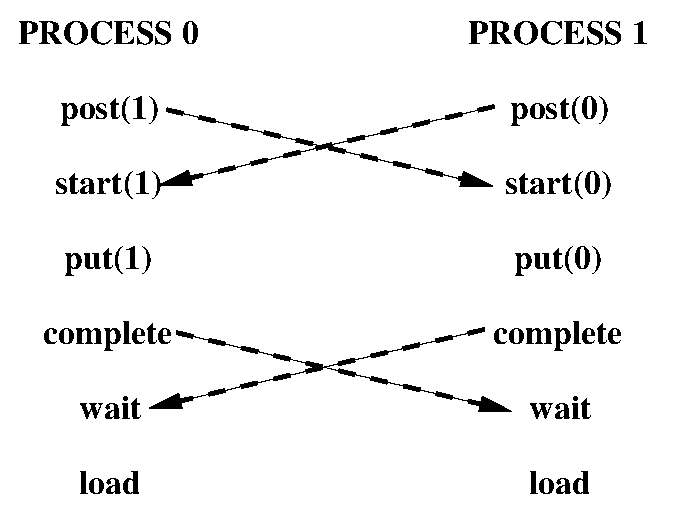
\includegraphics[width=3.0in]{figures/symmetric}}
\caption{Symmetric communication}
\label{fig:1sided-symmetric}
\end{figure}
Each \mpi/ process updates the window of the other \mpi/ process using a put
operation, then accesses its own window.  The post calls are
local.  Once the post calls occur, \RMA/
access to the windows is enabled, so that each \mpi/ process should complete
the sequence of start-put-complete.  Once these are done,
the wait calls should complete at both \mpi/ processes.  Thus, this
communication should not deadlock, irrespective of the amount of data 
transferred.

Assume, in the last example, that the order of the post and start
calls is reversed at each \mpi/ process.
Then, the code may deadlock, as
each \mpi/ process may not return from the start call, waiting for the matching post
to occur.
Similarly, the program will deadlock if the
order of the complete and 
wait calls is reversed at each \mpi/ process.

The following two examples illustrate the fact that the
synchronization between complete and wait is not symmetric: the wait
call returns only once the complete occurs, but not vice versa.
Consider the code illustrated in Figure~\ref{fig:1sided-deadlck1}.
\begin{figure}[t]
\centerline{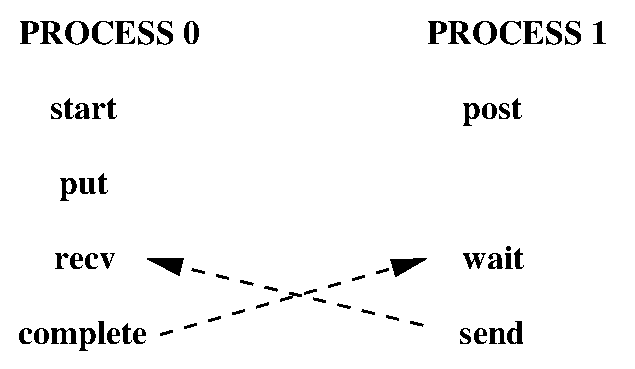
\includegraphics[width=2.5in]{figures/deadlck1}}

\caption{Deadlock situation}
\label{fig:1sided-deadlck1}
\end{figure}
This code will deadlock: the wait of process~1 completes only once process~0
calls complete, and the receive of process~0 completes once process~1
calls send.  Consider, on the other hand, the code
illustrated in Figure~\ref{fig:1sided-deadlck2}.
\begin{figure}[t]
\centerline{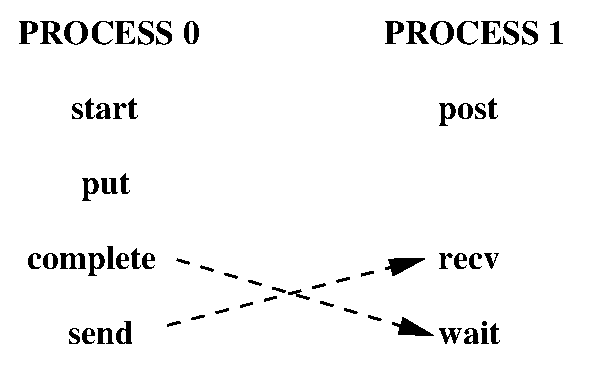
\includegraphics[width=2.5in]{figures/deadlck2}}

\caption{No deadlock}
\label{fig:1sided-deadlck2}
\end{figure}
This code will not deadlock.  Once process~1 calls post, then the
sequence start-put-complete on process~0 can proceed.
Process~0 will reach the send call, allowing the receive call of
process~1 to return.

\begin{rationale}
\MPI/ implementations must guarantee that an \mpi/ process makes 
\mpitermni{progress}\mpitermindex{progress!one-sided communication}\mpitermindex{one-sided communication!progress}\mpitermindex{semantics and correctness!one-sided communication!progress}
on all enabled communications it participates in,
while blocked on an \MPI/ call.  This is
true for send-receive communication and applies to \RMA/ communication
as well.  Thus, in the example in Figure~\ref{fig:1sided-deadlck2},
the put and complete calls of process~0 should complete
while process~1 is waiting for the receive operation to complete.  This may require the
involvement of process~1, e.g., to transfer the data.

A similar issue is whether such progress must occur
while an \mpi/ process is busy computing, or blocked in a
non-\MPI/ call.  Suppose that in the last example the send-receive
pair is replaced by a write-to-socket/read-from-socket pair.  Then
\MPI/ does not specify whether deadlock is avoided.
Suppose that the blocking
receive of process~1 is replaced by a very long compute loop.  Then,
according to one interpretation of
the \MPI/ standard, process~0 must return from the complete call after
a bounded delay, even if process~1 does not reach any \MPI/ call in
this period of time.  According to another interpretation, the
complete call may block until process~1 reaches the wait call, or
reaches another \MPI/ call.  The qualitative behavior is the same,
under both interpretations, unless an \mpi/ process is caught in an infinite compute loop, in which case the difference may not matter.
However, the quantitative expectations are different.
Different \MPI/ implementations reflect these different
interpretations.
While this ambiguity is unfortunate, the \MPI/ Forum decided not to define
which interpretation of the standard is the correct one, since the issue is
contentious.
See also \sectionref{subsec:terms:progress} on
\mpitermni{progress}\mpitermindex{progress!one-sided communication}\mpitermindex{one-sided communication!progress}\mpitermindex{semantics and correctness!one-sided communication!progress}.
\end{rationale}

The use of shared memory loads
and/or stores for synchronizing\mpitermindex{shared memory!loads/stores for synchronizing}
purposes between \MPI/ processes does not guarantee progress, and therefore
a \mpiterm{deadlock} may occur if an \MPI/ implementation
does not provide \mpiterm{strong progress}, as shown in \namedref{Example}{exa:sync-shared:deadlock}.

\begin{example}
\Exindex{C}{Deadlock due to synchronization through shared memory}{MPI\_Win\_shared\_query,MPI\_Win\_fence,MPI\_Buffer\_attach,MPI\_Buffer\_detach,MPI\_Bsend,MPI\_Recv}% 
\label{exa:sync-shared:deadlock}
Possible \mpitermni{deadlock} due to the use of a shared memory variable for synchronization.

\carg{comm\_sm} shall be a shared memory communicator (e.g., returned from a call to
\mpifunc{MPI\_COMM\_SPLIT\_TYPE} with \mpiarg{split\_type}\mpicode{=}\mpiconst{MPI\_COMM\_TYPE\_SHARED})  
with at least two \MPI/ processes.
\carg{win\_sm} is a shared memory window with the \carg{AckInRank0} as
window portion in \MPI/ process with rank \mpicode{0}.
The ranks in \carg{comm\_sm} and \carg{win\_sm} should be the same.
According to \sectionref{sec:1sided-semantics} rules~U\ref{rule:u2} and~U\ref{rule:u3},
a volatile store to \carg{AckInRank0} will be visible in the
other \MPI/ process without further \RMA/ calls.

\lstset{fancyvrb,language={[MPI]C},morefvcmdparams=\rlap 1}
%%HEADER
%%SKIP
%%ENDHEADER
\begin{Verbatim}[commandchars=\\\[\]]
int volatile_load(int *addr) {return *(volatile int *)addr;}
void volatile_store(int *addr, int val) {*((volatile int *)addr) = val;}

\wideunderline\textbf[Process with rank 0]                    \textbf[Process with rank 1]
MPI_Win_shared_query(win,              MPI_Win_shared_query(win,
   /*rank=*/ 0, ..., AckInRank0);         /*rank=*/ 0, ..., AckInRank0);
                                        
volatile_store(AckInRank0, 0);
MPI_Win_fence(win_sm)                  MPI_Win_fence(win_sm)
MPI_Buffer_attach(myHugeBuffer,...);
MPI_Bsend(myHugeMessage, ...,
          /*rank=*/ 1,..., comm_sm);   sleep(5); // to ensure
sleep(10); // to guarantee that          // that the MPI_Bsend
           // the while-loop starts      // in rank 0 returned
           // after rank 1 is
           // blocked in MPI_Recv      MPI_Recv(&myHugeMessage, ...                   
                                         /*rank=*/ 0, ..., comm_sm, ...);
                                       volatile_store(AckInRank0,222);
while(volatile_load(AckInRank0)!=222) 
          /*empty polling loop*/;
MPI_Buffer_detach(&pTemp, &size);
// deadlock                            // deadlock
\end{Verbatim}
\lstset{fancyvrb=false}

While the call to \mpifuncskip{MPI\_Recv} in the \MPI/ process with rank \mpicode{1} delays its return
(until an unspecific \MPI/ procedure call in the \MPI/ process with rank \mpicode{0} happens to send
the buffered data), the subsequent statement cannot change the value of the
shared window buffer \carg{AckInRank0}.
As long as this value is not changed, the while loop in the \MPI/ process with rank \mpicode{0}
will continue and therefore the next \MPI/ procedure call
(\mpifuncskip{MPI\_Buffer\_detach}) cannot happen, which is then a \mpitermni{deadlock}.
\end{example}

Note that both communication patterns
(A) \mpifuncskip{BSEND-RECV-DETACH}\mpifuncindex{MPI\_BSEND}\mpifuncindex{MPI\_RECV}\mpifuncindex{MPI\_BUFFER\_ATTACH}\mpifuncindex{MPI\_BUFFER\_DETACH}
and
(B) the shared memory store/load for synchronization purpose,
can be in different software layers and each layer would work properly,
but the combination of (A) and (B) can cause the \mpitermni{deadlock}. 

\subsection{Registers and Compiler Optimizations}
\label{sec:onesided-optimizations}
\label{sec:rma-register-opt}

\begin{users}
All the material in this section is an advice to users.
\end{users}

A coherence problem exists between variables kept in registers
and the memory values of these variables.  An
\RMA/ call may access a 
variable in memory (or cache), while the up-to-date value of this
variable is in register.  A get will not return the latest variable
value, and a put may be overwritten when the register is stored back
in memory.  Note that these issues are unrelated to the \RMA/ memory 
model; that is, these issues apply even if the memory model is 
\mpiconst{MPI\_WIN\_UNIFIED}.

The problem is illustrated in Example~\ref{ex:1sided-register}.

\begin{example}
\label{ex:1sided-register}
\Exindex{Neutral}{Register and Compiler Optimization}{MPI\_Win\_fence,MPI\_Put}%

In this example, variable \code{buff} is allocated in the register
\code{reg\_A} and therefore
\code{ccc} will have the old value of \code{buff} and not the new value
\code{777}.

\lstset{fancyvrb,language={[MPI]C},morefvcmdparams=\rlap 1}
%%HEADER
%%SKIP
%%ENDHEADER
\begin{Verbatim}[commandchars=\\\{\}]
\wideunderline\rlap{\textbf{Source of Process 1}}                         \rlap{\textbf{Source of Process 2}}                      \textbf{Executed in Process 2}
bbbb = 777               buff = 999            reg\_A:=999
call MPI_WIN_FENCE       call MPI_WIN_FENCE
call MPI_PUT(bbbb                              stop appl.\,thread
 into buff of process 2)                       buff:=777 in PUT handler
                                               continue appl.\,thread
call MPI_WIN_FENCE       call MPI_WIN_FENCE
                         ccc = buff            ccc:=reg\_A
\end{Verbatim}
\lstset{fancyvrb=false}
\end{example}

This problem, which also afflicts in some cases
send/receive communication, is discussed more at length in 
Section~\ref{sec:misc-register}.

Programs written in C avoid this problem, because of the semantics of C. 
Many Fortran compilers will avoid this
problem, without disabling compiler optimizations.
However, in order to avoid register coherence problems in a completely
portable manner, users should  restrict
their use of \RMA/ windows to variables stored in 
modules or \ftype{COMMON} blocks.
To prevent problems with the argument copying and register
optimization done by Fortran compilers, please note the hints in 
Sections~\ref{sec:misc-problems}--\ref{sec:f90-problems:comparison-with-C}.
%%% See comments in pt2pt on why the commented text is both incorrect and
%% unnecessary
%% especially in 
%% Sections~\ref{sec:misc-sequence} and~\ref{sec:f90-problems:vector-subscripts}
%% on pages~\pageref{sec:misc-sequence}--\pageref{sec:f90-problems:vector-subscripts}
%% about ``{\sf Problems Due to Data Copying and Sequence Association with Subscript Triplets}''
%% and ``{\sf Vector Subscripts}'',
%% and in Sections~\ref{sec:misc-register} to~\ref{sec:f90-problems:perm-data-movements}
%% on pages~\pageref{sec:misc-register} to~\pageref{sec:f90-problems:perm-data-movements} 
%% about ``{\sf Optimization Problems}'', ``{\sf Code Movements and Register Optimization}'', 
%% ``{\sf Temporary Data Movements}'' and ``{\sf Permanent Data Movements}''.  
%\sectionrange{sec:f90-problems:code-movements:solutions}{sec:f90-problems:volatile}
% These are unnumbered subsubsections
In Section~\ref{sec:f90-problems:code-movements},
\nameref{sec:f90-problems:code-movements:solutions} to \nameref{sec:f90-problems:volatile}
discuss several solutions for the problem in this example.


\section{Examples}
\label{sec:onesided_examples}

\begin{example}
\label{ex:1sided-fence}
\Exindex{C}{Put with fence}{MPI\_Win\_fence,MPI\_Put}%
The following example shows a generic loosely synchronous, iterative
code, using \mpifunc{MPI\_WIN\_FENCE} for synchronization.  The window at each \mpi/ process
consists of array \code{A}, which contains the origin and target buffers of
the
put operations.

%%HEADER
%%LANG: C
%%FRAGMENT
%%SKIPELIPSIS
%%DECL: int converged(int), i, A; MPI_Win win;
%%DECL: int toneighbors, toneighbor[10], frombuf[10]; int update(int);
%%DECL: MPI_Datatype totype[10], fromtype[10];
%%DECL: MPI_Aint todisp[10];
%%ENDHEADER
\begin{lstlisting}[language={[MPI]C}]
...
while (!converged(A)) {
  update(A);
  MPI_Win_fence(MPI_MODE_NOPRECEDE, win);
  for(i=0; i < toneighbors; i++)
    MPI_Put(&frombuf[i], 1, fromtype[i], toneighbor[i],
            todisp[i], 1, totype[i], win);
  MPI_Win_fence((MPI_MODE_NOSTORE | MPI_MODE_NOSUCCEED), win);
}
\end{lstlisting}
The same code could be written with get rather than put.  Note that,
during the communication phase, each
window is concurrently read  (as origin buffer of puts) and written
(as target buffer of puts).  This is OK, provided that there is no
overlap between the target buffer of a put and another communication 
buffer.
\end{example}

\begin{example}
\label{ex:1sided-split}
\Exindex{C}{Get with fence}{MPI\_Win\_fence,MPI\_Get}%
Same generic example, with more computation/communication overlap.  We
assume that the update phase is broken into two
subphases: the first, 
where the ``boundary,'' which is involved in communication, is updated, and
the second, where the ``core,'' which neither
uses nor provides 
communicated data, is updated.
%%HEADER
%%LANG: C
%%FRAGMENT
%%SKIPELIPSIS
%%DECL: int converged(int), i, fromneighbors, A; MPI_Win win;
%%DECL: MPI_Datatype totype[10], fromtype[10]; int tobuf[10];
%%DECL: int fromneighbor[10]; MPI_Aint fromdisp[10];
%%DECL: void update_boundary(int), update_core(int);
%%ENDHEADER
\begin{lstlisting}[language={[MPI]C}]
...
while (!converged(A)) {
  update_boundary(A);
  MPI_Win_fence((MPI_MODE_NOPUT | MPI_MODE_NOPRECEDE), win);
  for(i=0; i < fromneighbors; i++)
    MPI_Get(&tobuf[i], 1, totype[i], fromneighbor[i],
            fromdisp[i], 1, fromtype[i], win);
  update_core(A);
  MPI_Win_fence(MPI_MODE_NOSUCCEED, win);
}
\end{lstlisting}
The get communication can be concurrent with the core update, since
they do not access the same locations, and the local update of the
origin buffer by the get operation can be concurrent with the local update
of the core by the \code{update\_core} call.  In order to get similar
overlap with put communication we would need to use separate windows
for the core and for the boundary.
This is required 
because we do not allow local stores to be concurrent with puts
on the same, or on overlapping, windows.
\end{example}

\begin{example}
\Exindex{C}{Put with PSCW}{MPI\_Win\_post,MPI\_Win\_start,MPI\_Put,MPI\_Win\_complete,MPI\_Win\_wait}%
Same code as in Example~\ref{ex:1sided-fence},
rewritten using post-start-complete-wait.
%%HEADER
%%LANG: C
%%FRAGMENT
%%SKIPELIPSIS
%%DECL: int converged(int), i, toneighbors; MPI_Group fromgroup, togroup;
%%DECL: int A; MPI_Datatype fromtype[10], totype[10]; MPI_Win win;
%%DECL: int frombuf[10], toneighbor[10]; MPI_Aint todisp[10];
%%DECL: void update(int);
%%ENDHEADER
\begin{lstlisting}[language={[MPI]C}]
...
while (!converged(A)) {
  update(A);
  MPI_Win_post(fromgroup, 0, win);
  MPI_Win_start(togroup, 0, win);
  for(i=0; i < toneighbors; i++)
    MPI_Put(&frombuf[i], 1, fromtype[i], toneighbor[i],
            todisp[i], 1, totype[i], win);
  MPI_Win_complete(win);
  MPI_Win_wait(win);
}
\end{lstlisting}
\end{example}

\begin{example}
\Exindex{C}{Get with PSCW}{MPI\_Win\_post,MPI\_Win\_start,MPI\_Get,MPI\_Win\_complete,MPI\_Win\_wait}%
Same example, with post-start-complete-wait, as in Example~\ref{ex:1sided-split}.
%%HEADER
%%LANG: C
%%FRAGMENT
%%SKIPELIPSIS
%%DECL: int converged(int), A; MPI_Group togroup, fromgroup; MPI_Win win; 
%%DECL: int i, fromneighbors; MPI_Datatype totype[10], fromtype[10];
%%DECL: MPI_Aint fromdisp[10]; int tobuf[10], fromneighbor[10];
%%DECL: void update_boundary(int), update_core(int);
%%ENDHEADER
\begin{lstlisting}[language={[MPI]C}]
...
while (!converged(A)) {
  update_boundary(A);
  MPI_Win_post(togroup, MPI_MODE_NOPUT, win);
  MPI_Win_start(fromgroup, 0, win);
  for(i=0; i < fromneighbors; i++)
    MPI_Get(&tobuf[i], 1, totype[i], fromneighbor[i],
            fromdisp[i], 1, fromtype[i], win);
  update_core(A);
  MPI_Win_complete(win);
  MPI_Win_wait(win);
}
\end{lstlisting}
\end{example}

\begin{example}
\Exindex[Double buffer in \RMA/]{C}{Double buffer in RMA@Double buffer in \RMA/}{MPI\_Barrier,MPI\_Win\_post,MPI\_Win\_start,MPI\_Get,MPI\_Win\_complete,MPI\_Win\_wait}%
A checkerboard, or double buffer  communication pattern, that allows
more computation/communication overlap.  Array \code{A0} is updated
using values of array \code{A1}, and vice versa.  We assume that communication is symmetric: if process A gets data from process B, then process B gets data from process A.  Window \code{wini} consists of array \code{Ai}.
%%HEADER
%%LANG: C
%%SKIPELIPSIS
%%FRAGMENT
%%DECL: MPI_Group neighbors; MPI_Win win0, win1; MPI_Comm comm0;
%%DECL: int converged(int,int); int A0, A1, i; int update2(int,int);
%%DECL: int fromneighbors;
%%DECL: int update1(int);
%%DECL: MPI_Datatype totype0[10], fromtype0[10], totype1[10], fromtype1[10]; 
%%DECL: MPI_Aint fromdisp0[10], fromdisp1[10]; int tobuf0[10], tobuf1[10];
%%DECL: int neighbor[10];
%%ENDHEADER
\begin{lstlisting}[language={[MPI]C}]
...
if (!converged(A0,A1))
  MPI_Win_post(neighbors, (MPI_MODE_NOCHECK | MPI_MODE_NOPUT), win0);
MPI_Barrier(comm0);
/* the barrier is needed because the start call inside the
loop uses the nocheck option */
while (!converged(A0, A1)) {
  /* communication on A0 and computation on A1 */
  update2(A1, A0); /* local update of A1 that depends on A0 (and A1) */
  MPI_Win_start(neighbors, MPI_MODE_NOCHECK, win0);
  for(i=0; i < fromneighbors; i++)
    MPI_Get(&tobuf0[i], 1, totype0[i], neighbor[i],
            fromdisp0[i], 1, fromtype0[i], win0);
  update1(A1); /* local update of A1 that is
                  concurrent with communication that updates A0 */ 
  MPI_Win_post(neighbors, (MPI_MODE_NOCHECK | MPI_MODE_NOPUT), win1);
  MPI_Win_complete(win0);
  MPI_Win_wait(win0);

  /* communication on A1 and computation on A0 */
  update2(A0, A1); /* local update of A0 that depends on A1 (and A0) */
  MPI_Win_start(neighbors, MPI_MODE_NOCHECK, win1);
  for(i=0; i < fromneighbors; i++)
    MPI_Get(&tobuf1[i], 1, totype1[i], neighbor[i],
            fromdisp1[i], 1, fromtype1[i], win1);
  update1(A0); /* local update of A0 that depends on A0 only,
                 concurrent with communication that updates A1 */
  if (!converged(A0,A1))
    MPI_Win_post(neighbors, (MPI_MODE_NOCHECK | MPI_MODE_NOPUT), win0);
  MPI_Win_complete(win1);
  MPI_Win_wait(win1);
}
\end{lstlisting}

An \mpi/ process posts the local window associated with
\code{win0} before it completes \RMA/ accesses to
the remote windows associated with \code{win1}.
When the call to \mpifunc{MPI\_WIN\_WAIT} on \code{win1}
returns, then all neighbors of the calling \mpi/ process have posted the
windows associated with \code{win0}. Conversely, when the 
call to \mpifunc{MPI\_WIN\_WAIT} on \code{win0} returns, then all neighbors of the calling \mpi/ process
have posted the windows associated with \code{win1}.
Therefore, the \mpiconst{MPI\_MODE\_NOCHECK} option can be used with the calls to
\mpifunc{MPI\_WIN\_START}.

Put operations can be used, instead of get operations, if the area of array
\code{A0} (resp.\ \code{A1}) used by \code{update(A1, A0)}
(resp.\ \code{update(A0, A1)}) is disjoint from the area
modified by the \RMA/ operation.  On some systems, a put operation may be
more efficient than a get operation, as it requires information exchange
only in one direction.

\end{example}

In the next several examples, for conciseness, the expression
\lstset{fancyvrb,language={[MPI]C},morefvcmdparams=\textbf 1}
%%HEADER
%%SKIP
%%ENDHEADER
\begin{Verbatim}
z = MPI_Get_accumulate(...)
\end{Verbatim}
\lstset{fancyvrb=false}
means to perform a get-accumulate operation with the result
buffer (given by \mpiarg{result\_addr} in the description of
\mpifunc{MPI\_GET\_ACCUMULATE}) on the left side of the
assignment, in 
this case, \mpiarg{z}.  This format is also used with
\mpifunc{MPI\_COMPARE\_AND\_SWAP} and \mpifunc{MPI\_COMM\_SIZE}.
Process B$\ldots$ refers to any process other than A.

\begin{example}
\Exindex{Neutral}{Counting semaphore (nonscalable)}{MPI\_Barrier,MPI\_Accumulate,MPI\_Get\_accumulate,MPI\_Win\_flush,MPI\_Win\_sync}%
%Example 2 (rule 6).
The following example implements a naive, nonscalable counting
semaphore.  The example demonstrates the use of
\mpifunc{MPI\_WIN\_SYNC} to manipulate the public copy of \code{X}, as well
as \mpifunc{MPI\_WIN\_FLUSH} to complete operations without closing the
access epoch opened with \mpifunc{MPI\_WIN\_LOCK\_ALL}.  To avoid the
rules regarding synchronization of the public and private copies of
windows, \mpifunc{MPI\_ACCUMULATE} and \mpifunc{MPI\_GET\_ACCUMULATE}
are used to write to or read from the local public copy.
\lstset{fancyvrb,language={[MPI]C},morefvcmdparams=\rlap 1}
%%HEADER
%%SKIP
%%ENDHEADER
\begin{Verbatim}[commandchars=\\\{\}]
\wideunderline\rlap{\textbf{Process A}}                                          \textbf{Process B...}
MPI_Win_lock_all                          MPI_Win_lock_all
window location X
X=MPI_Comm_size()
MPI_Win_sync
MPI_Barrier                               MPI_Barrier

MPI_Accumulate(X, MPI_SUM, -1)            MPI_Accumulate(X, MPI_SUM, -1)

stack variable z                          stack variable z
do                                        do
  z = MPI_Get_accumulate(X,                 z = MPI_Get_accumulate(X,
       MPI_NO_OP, 0)                             MPI_NO_OP, 0)
  MPI_Win_flush(A)                          MPI_Win_flush(A)
while(z!=0)                               while(z!=0)

MPI_Win_unlock_all                        MPI_Win_unlock_all
\end{Verbatim}
\lstset{fancyvrb=false}
\end{example}

\begin{example}
\Exindex[Critical region with \RMA/]{Neutral}{Critical region with RMA@Critical region with \RMA/}{MPI\_Barrier,MPI\_Accumulate,MPI\_Win\_sync,MPI\_Get\_accumulate,MPI\_Win\_flush,MPI\_Win\_flush\_all}%
%Example 2 (rule 6).
Implementing a critical region between two \mpi/ processes (Peterson's
algorithm).  Despite their appearance in the
following example, \mpifunc{MPI\_WIN\_LOCK\_ALL} and
\mpifunc{MPI\_WIN\_UNLOCK\_ALL} are not collective calls, but it is
frequently useful to open shared access epochs to all \mpi/ processes from
all other \mpi/ processes in a window.  Once the access epochs are
opened, accumulate operations as well as flush and sync
synchronization can be used to read from or write to the
public copy of the window.
\lstset{fancyvrb,language={[MPI]C},morefvcmdparams=\rlap 1}
%%HEADER
%%SKIP
%%ENDHEADER
\begin{Verbatim}[commandchars=\\\{\}]
\wideunderline\rlap{\textbf{Process A}}                                      \textbf{Process B}
window location X                     window location Y
window location T

MPI_Win_lock_all                      MPI_Win_lock_all
X=1                                   Y=1
MPI_Win_sync                          MPI_Win_sync
MPI_Barrier                           MPI_Barrier
MPI_Accumulate(T, MPI_REPLACE, 1)     MPI_Accumulate(T, MPI_REPLACE, 0)
stack variables t,y                   stack variable t,x
t=1                                   t=0
y=MPI_Get_accumulate(Y,               x=MPI_Get_accumulate(X,
   MPI_NO_OP, 0)                         MPI_NO_OP, 0)
while(y==1 && t==1) do                while(x==1 && t==0) do
  y=MPI_Get_accumulate(Y,               x=MPI_Get_accumulate(X,
     MPI_NO_OP, 0)                         MPI_NO_OP, 0)
  t=MPI_Get_accumulate(T,               t=MPI_Get_accumulate(T,
     MPI_NO_OP, 0)                         MPI_NO_OP, 0)
  MPI_Win_flush_all                     MPI_Win_flush(A)
done                                  done
// critical region                    // critical region
MPI_Accumulate(X, MPI_REPLACE, 0)     MPI_Accumulate(Y, MPI_REPLACE, 0)
MPI_Win_unlock_all                    MPI_Win_unlock_all
\end{Verbatim}
\lstset{fancyvrb=false}
\end{example}

\begin{example}
\Exindex{Neutral}{Critical region with Compare-and-Swap}{MPI\_Barrier,MPI\_Win\_sync,MPI\_Compare\_and\_swap,MPI\_Win\_flush}%
%Example 2 (rule 6).
Implementing a critical region between multiple \mpi/ processes with compare
and swap.  The call to \mpifunc{MPI\_WIN\_SYNC} is necessary on
Process A after local initialization of \code{A} to guarantee the public copy
has been updated with the initialization value found in the private
copy.  It would also be valid to call \mpifunc{MPI\_ACCUMULATE} with
\mpiconst{MPI\_REPLACE} to directly initialize the public copy.  A call
to \mpifunc{MPI\_WIN\_FLUSH} would be necessary to assure \code{A} in the
public copy of Process A had been updated before the barrier.
\lstset{fancyvrb,language={[MPI]C},morefvcmdparams=\rlap 1}
%%HEADER
%%SKIP
%%ENDHEADER
\begin{Verbatim}[commandchars=\\\{\}]
\wideunderline\rlap{\textbf{Process A}}                                      \textbf{Process B...}
MPI_Win_lock_all                      MPI_Win_lock_all
atomic location A
A=0
MPI_Win_sync
MPI_Barrier                           MPI_Barrier
stack variable r = 1                  stack variable r = 1
while(r != 0) do                      while(r != 0) do
  r = MPI_Compare_and_swap(A, 0, 1)     r = MPI_Compare_and_swap(A, 0, 1)
  MPI_Win_flush(A)                      MPI_Win_flush(A)
done                                  done
// critical region                    // critical region
r = MPI_Compare_and_swap(A, 1, 0)     r = MPI_Compare_and_swap(A, 1, 0)
MPI_Win_unlock_all                    MPI_Win_unlock_all
\end{Verbatim}
\lstset{fancyvrb=false}
\end{example}
% Note that at one point we required the same operation in accumulates
% - that restriction is now gone.
%{Note that
%  \mpifunc{MPI\_Compare\_and\_swap} must be used to release the mutex
%  at the end, rather than using either \mpifunc{MPI\_Put} or
%  \mpifunc{MPI\_Accumulate} with \mpiconst{MPI\_REPLACE}, because
%  ordering }

\begin{example}\label{ex:shmem-sync}%
The following example demonstrates the proper synchronization in the
unified memory model when a data transfer is implemented with load and
store accesses in the case of windows in \mpiterm{shared memory} (instead of using \mpifuncshort{MPI\_PUT} or
\mpifuncshort{MPI\_GET}) and the synchronization between \mpi/ processes is performed using
point-to-point communication. The synchronization between \mpi/ processes
must be supplemented with a memory synchronization through calls to
\mpifunc{MPI\_WIN\_SYNC}, which act locally as a processor-memory barrier. In
Fortran, if \mpiconst{MPI\_ASYNC\_PROTECTS\_NONBLOCKING} is
\exindex{MPI\_ASYNC\_PROTECTS\_NONBLOCKING}%
\code{.FALSE.}
or the variable \code{X} is not declared as \ftype{ASYNCHRONOUS},
\exindex{ASYNCHRONOUS}%
reordering of the accesses to the
variable \code{X} must be prevented with \mpifunc{MPI\_F\_SYNC\_REG}
operations. (No equivalent function is needed in C.)

The variable \code{X} is contained within a \mpitermni{shared memory window}\mpitermindex{shared memory!window} and \code{X}
corresponds to the same memory location at both processes. The first call to
\mpifunc{MPI\_WIN\_SYNC} performed by process A ensures completion of
the load/store accesses issued by process A. The first call to \mpifunc{MPI\_WIN\_SYNC}
performed by process B ensures that process A's updates to \code{X}
are visible to process B.
Similarly, the second call to \mpifunc{MPI\_WIN\_SYNC} on each process ensures
correct ordering of the point-to-point communication and thus that the load/store
operations on process B have completed before any subsequent
load/store accesses to the variable \code{X} in process A.

% MPI_F_SYNC_REG only has Fortran bindings
\Exindex{Neutral}{Shared memory windows}{MPI\_Win\_lock\_all,MPI\_F\_SYNC\_REG}%
\exindex{MPI\_Win\_sync!shared memory windows}%
\exindex{Shared memory windows!MPI\_Win\_sync}%
\lstset{fancyvrb,language={[MPI]Fortran},morefvcmdparams=\rlap 1}
%%HEADER
%%SKIP
%%ENDHEADER
\begin{Verbatim}[commandchars=\\\{\}]
\wideunderline\rlap{\textbf{Process A}}                                 \textbf{Process B}
MPI_WIN_LOCK_ALL(                MPI_WIN_LOCK_ALL(
      MPI_MODE_NOCHECK,win)            MPI_MODE_NOCHECK,win)

DO ...                           DO ...
  X=...

  MPI_F_SYNC_REG(X)
  MPI_WIN_SYNC(win)
  MPI_SEND                         MPI_RECV
                                   MPI_WIN_SYNC(win)
                                   MPI_F_SYNC_REG(X)

                                   print X

                                   MPI_F_SYNC_REG(X)
                                   MPI_WIN_SYNC(win)
  MPI_RECV                         MPI_SEND
  MPI_WIN_SYNC(win)
  MPI_F_SYNC_REG(X)
END DO                           END DO

MPI_WIN_UNLOCK_ALL(win)          MPI_WIN_UNLOCK_ALL(win)
\end{Verbatim}
\lstset{fancyvrb=false}
\end{example}

\begin{example}
\Exindex{C}{Requests in RMA@Requests in \RMA/}{MPI\_Win\_lock\_all,MPI\_Rget,MPI\_Rput,MPI\_Win\_unlock\_all,MPI\_Waitall,MPI\_Waitany}%
The following example shows how request-based operations can be used
to overlap communication with computation.  Each \mpi/ process fetches,
processes, and writes the result for \code{NSTEPS} chunks of data.  Instead
of a single buffer, \code{M} local buffers are used to allow up to \code{M}
communication operations to overlap with computation. 

%%HEADER
%%LANG: C
%%FRAGMENT
%%SUBST:\.\.\.:j
%%DECL: #define M 1
%%DECL: #define N 1
%%DECL: const int NSTEPS=10; int target;
%%DECL: void compute(int,double[],int);
%%ENDHEADER
\begin{lstlisting}[language={[MPI]C}]
int         i, j;
MPI_Win     win;
MPI_Request put_req[M] = { MPI_REQUEST_NULL };
MPI_Request get_req;
double      *baseptr;
double      data[M][N];

MPI_Win_allocate(NSTEPS*N*sizeof(double), sizeof(double), MPI_INFO_NULL,
                 MPI_COMM_WORLD, &baseptr, &win);

MPI_Win_lock_all(0, win);

for (i = 0; i < NSTEPS; i++) {
 if (i<M)
   j=i;
 else
   MPI_Waitany(M, put_req, &j, MPI_STATUS_IGNORE);

 MPI_Rget(data[j], N, MPI_DOUBLE, target, i*N, N, MPI_DOUBLE, win,
          &get_req);
 MPI_Wait(&get_req,MPI_STATUS_IGNORE);
 compute(i, data[j], ...);
 MPI_Rput(data[j], N, MPI_DOUBLE, target, i*N, N, MPI_DOUBLE, win,
          &put_req[j]);
}

MPI_Waitall(M, put_req, MPI_STATUSES_IGNORE);
MPI_Win_unlock_all(win);
\end{lstlisting}
\end{example}

\begin{example}
The following example constructs a distributed shared linked list using dynamic
windows.  Initially process~0 creates the head of the list, attaches it to
the window, and broadcasts the pointer to all \mpi/ processes.  All \mpi/ processes then
concurrently append \code{N} new elements to the list.  When an \mpi/
process attempts to 
attach its element to the tail of the list it may discover that its tail pointer
is stale and it must chase ahead to the new tail before the element can be
attached.
This example requires some modification to
work in an environment where the layout of the structures is different on
different \mpi/ processes.

\Exindex{C}{Linked list in RMA@Linked list in \RMA/}{MPI\_Win\_create\_dynamic,MPI\_Alloc\_mem,MPI\_Free\_mem,MPI\_Win\_attach,MPI\_Win\_detach,MPI\_Win\_lock\_all,MPI\_Compare\_and\_swap,MPI\_Accumulate,MPI\_Get\_accumulate,MPI\_Win\_flush,MPI\_Win\_unlock\_all,MPI\_Aint\_add}%
%%HEADER
%%LANG: C
%%SUBST:\.\.\.:
%%TAIL: return 0;}
%%TOP: #include <stddef.h>
%%ENDHEADER
\begin{lstlisting}[language={[MPI]C},basicstyle=\lstsmall]
...
#define NUM_ELEMS 10

#define LLIST_ELEM_NEXT_RANK ( offsetof(llist_elem_t, next) + \
                               offsetof(llist_ptr_t, rank) )
#define LLIST_ELEM_NEXT_DISP ( offsetof(llist_elem_t, next) + \
                               offsetof(llist_ptr_t, disp) )

/* Linked list pointer */
typedef struct {
  MPI_Aint disp;
  int      rank;
} llist_ptr_t;

/* Linked list element */
typedef struct {
  llist_ptr_t next;
  int value;
} llist_elem_t;

const llist_ptr_t nil = { (MPI_Aint) MPI_BOTTOM, -1 };

/* List of locally allocated list elements. */
static llist_elem_t **my_elems = NULL;
static int my_elems_size  = 0;
static int my_elems_count = 0;

/* Allocate a new shared linked list element */
MPI_Aint alloc_elem(int value, MPI_Win win) {
  MPI_Aint disp;
  llist_elem_t *elem_ptr;

  /* Allocate the new element and register it with the window */
  MPI_Alloc_mem(sizeof(llist_elem_t), MPI_INFO_NULL, &elem_ptr);
  elem_ptr->value = value;
  elem_ptr->next  = nil;
  MPI_Win_attach(win, elem_ptr, sizeof(llist_elem_t));

  /* Add the element to the list of local elements so we can free
     it later. */
  if (my_elems_size == my_elems_count) {
    my_elems_size += 100;
    my_elems = realloc(my_elems, my_elems_size*sizeof(void*));
  }
  my_elems[my_elems_count] = elem_ptr;
  my_elems_count++;

  MPI_Get_address(elem_ptr, &disp);
  return disp;
}

int main(int argc, char *argv[]) {
  int           procid, nproc, i;
  MPI_Win       llist_win;
  llist_ptr_t   head_ptr, tail_ptr;

  MPI_Init(&argc, &argv);

  MPI_Comm_rank(MPI_COMM_WORLD, &procid);
  MPI_Comm_size(MPI_COMM_WORLD, &nproc);

  MPI_Win_create_dynamic(MPI_INFO_NULL, MPI_COMM_WORLD, &llist_win);

  /* Process 0 creates the head node */
  if (procid == 0)
    head_ptr.disp = alloc_elem(-1, llist_win);

  /* Broadcast the head pointer to everyone */
  head_ptr.rank = 0;
  MPI_Bcast(&head_ptr.disp, 1, MPI_AINT, 0, MPI_COMM_WORLD);
  tail_ptr = head_ptr;

  /* Lock the window for shared access to all targets */
  MPI_Win_lock_all(0, llist_win);

  /* All processes concurrently append NUM_ELEMS elements to the list */
  for (i = 0; i < NUM_ELEMS; i++) {
    llist_ptr_t new_elem_ptr;
    int success;

    /* Create a new list element and attach it to the window */
    new_elem_ptr.rank = procid;
    new_elem_ptr.disp = alloc_elem(procid, llist_win);

    /* Append the new node to the list.  This might take multiple 
       attempts if others have already appended and our tail pointer 
       is stale. */
    do {
      llist_ptr_t next_tail_ptr = nil;

      MPI_Compare_and_swap((void*) &new_elem_ptr.rank, (void*) &nil.rank,
          (void*)&next_tail_ptr.rank, MPI_INT, tail_ptr.rank,
          MPI_Aint_add(tail_ptr.disp, LLIST_ELEM_NEXT_RANK),
          llist_win);

      MPI_Win_flush(tail_ptr.rank, llist_win);
      success = (next_tail_ptr.rank == nil.rank);

      if (success) {
        MPI_Accumulate(&new_elem_ptr.disp, 1, MPI_AINT, tail_ptr.rank,
            MPI_Aint_add(tail_ptr.disp, LLIST_ELEM_NEXT_DISP), 1,
            MPI_AINT, MPI_REPLACE, llist_win);

        MPI_Win_flush(tail_ptr.rank, llist_win);
        tail_ptr = new_elem_ptr;

      } else {
        /* Tail pointer is stale, fetch the displacement.  May take
           multiple tries if it is being updated. */
        do {
          MPI_Get_accumulate(NULL, 0, MPI_AINT, &next_tail_ptr.disp,
              1, MPI_AINT, tail_ptr.rank,
              MPI_Aint_add(tail_ptr.disp, LLIST_ELEM_NEXT_DISP),
              1, MPI_AINT, MPI_NO_OP, llist_win);

          MPI_Win_flush(tail_ptr.rank, llist_win);
        } while (next_tail_ptr.disp == nil.disp);
        tail_ptr = next_tail_ptr;
      }
    } while (!success);
  }

  MPI_Win_unlock_all(llist_win);
  MPI_Barrier(MPI_COMM_WORLD);

  /* Free all the elements in the list */
  for ( ; my_elems_count > 0; my_elems_count--) {
    MPI_Win_detach(llist_win,my_elems[my_elems_count-1]);
    MPI_Free_mem(my_elems[my_elems_count-1]);
  }
  MPI_Win_free(&llist_win);
...
\end{lstlisting}
\end{example}

% LocalWords:  RMA MPI noncoherent SMP ALLOC MEM baseptr Alloc mem Aint IERROR
% LocalWords:  const FRR malloc IERR sizeof disp comm int GB attr ierror addr
% LocalWords:  datatype datatypes MAPVALS otype oindex ttype tindex sizeofreal
% LocalWords:  ierr INIT eps NOPRECEDE bool no-op NT NOCHECK NOSTORE NOPUT noput
% LocalWords:  NOSUCCEED nonportably nocheck nostore noprecede nosucceed todisp
% LocalWords:  toneighbors frombuf fromtype toneighbor totype subphases tobuf
% LocalWords:  fromneighbors fromneighbor fromdisp fromgroup togroup wini Ai
% LocalWords:  resp LOCKTYPE locktype NOMEM nonoverlapping Nonconflicting
% LocalWords:  deadlck

